\documentclass[fontsize=12pt,openright,twoside,paper=a4,BCOR=1cm,parskip=half]{scrbook}

\newcommand{\authornamefirst}{Mathieu}
\newcommand{\authornamemiddle}{}
\newcommand{\authornamelast}{Gaillard}
\newcommand{\worktitle}{Perceptual Hashing using Convolutional Neural Networks for Large Scale Reverse Image Search}
\newcommand{\thesistype}{Masterarbeit}
\newcommand{\thesisdate}{September 2017}
\newcommand{\thesisprof}{Prof. Dr. Michael Granitzer}
\newcommand{\thesissecondprof}{Prof. Dr. Lionel Brunie}
\newcommand{\supervisor}{Dr. El{\"o}d Egyed-Zsigmond}
\newcommand{\chair}{Chair of Data Science}

\newcommand{\contactprofone}{
\thesisprof \\
\chair \\
Universit\"at Passau \\
EMail:~{\small \url{michael.granitzer@uni-passau.de}}  \\
Web:~{\small
\url{http://mgrani.github.io}}\\}

\newcommand{\contactproftwo}{
\thesissecondprof \\
Institut National des Sciences Appliqu�es de Lyon \\
EMail:~{\small \url{lionel.brunie@insa-lyon.fr}}  \\
Web:~{\small
\url{http://liris.cnrs.fr/lionel.brunie}}\\}


\newcommand{\contactsupervisor}{
\supervisor \\
Institut National des Sciences Appliqu�es de Lyon \\
EMail:~{\small \url{elod.egyed-zsigmond@insa-lyon.fr}}  \\
Web:~{\small
\url{http://liris.cnrs.fr/eegyedzs}}\\}



%%%%%%%%%%%%%%%%%%%%%%%%%%%%%%%%%%%%%%%%%%%%%%%%%%%%%%%%%%%%

% PACKAGES:





% Use English :

% Use list of tabels, etc. in table of contents:
\usepackage{tocbibind}
% Encoder:????
\usepackage[latin1]{inputenc}
% Index-generation
\usepackage{makeidx}
% Einbinden von URLs:
\usepackage{url}
% Include .eps-files (needed also for the CNACC-logo):
%\usepackage{epsf}
% Special \LaTex symbols (e.g. \BibTeX):
\usepackage{doc}
% Include Graphic-files:
%\usepackage{graphics}
% Include Graphic-files:
\usepackage{graphicx}
% Include doc++ generated tex-files:
%\usepackage{docxx}
% Include PDF links

%mathstuff
\usepackage[cmex10]{amsmath}
\usepackage{amsfonts}
\usepackage{amssymb}

%hyperref for nice PDF output
\usepackage[pdftex, bookmarks=true]{hyperref}

\usepackage{listings}
\usepackage{scrhack}
\usepackage{rotating}
\usepackage{xcolor}
\usepackage{bbm}

%%%%%%%%%%%%%%%%%%%%%%%%%%%%%%%%%%%%%%%%%%%%%%%%%%%%%%%%%%%%

% OTHER SETTINGS:

% Pagestyle:
\pagestyle{headings}

% Avoid 'overhang':
\sloppy

% Choose language
\newcommand{\setlang}[1]{\selectlanguage{#1}\nonfrenchspacing}

\usepackage[USenglish]{babel}


\setlang{USenglish}
%\setlang{german}

\newcommand\norm[1]{\lVert#1\rVert}
\DeclareMathOperator*{\argmin}{arg\,min}

%%%%%%%%%%%%%%%%%%%%%%%%%%%%%%%%%%%%%%%%%%%%%%%%%%%%%%%%%%%%

% TITLE:

\begin{document}

\thispagestyle{empty}
\newpage

\vspace{1cm}

\begin{center}
	\begin{tabular}{lr}
	
\includegraphics[width=6.5cm]{img/logouni.pdf}
	&
	
\includegraphics[width=6.5cm]{img/logoinsa.png}
	\end{tabular}

	\vspace{3cm}
	\Large{University of Passau}
	\\
	\Large{Faculty of Computer Science and Mathematics}
	\\
	\vspace{0.3cm}
	\Large{\textbf{\chair}}
	\\
	\Large{\thesisprof}
	\\

	\vspace{0.6cm}
	\Large{INSA Lyon}
	\\
	\Large{D{\'e}partement Informatique}
	\\

	\vspace{0.6cm}
	\Large{Double Master Program}
\end{center}


\vspace{3cm}

\begin{center}
	\Huge{\textbf{\thesistype}} % Master Thesis, Programming Project
\end{center}

\begin{center}
	\settowidth{\baselineskip}{0.4cm}
	\LARGE{\worktitle}
	\\
	\Large{\authornamefirst~\authornamemiddle~\authornamelast}
\end{center}

\vfill {% \settowidth{\baselineskip}{0.2cm}

\vfill


\large{
\begin{tabular}[l]{llll}

Date:       & \thesisdate %%(\LaTeX{}$2_\epsilon$ run \today)
\smallskip \\
Supervisors:   & \thesisprof \\
&\thesissecondprof \\
	& \supervisor \\
\end{tabular}}
} \cleardoublepage
%%%%%%%%%%%%%%%%%%%%%%%%%%%%%%%%%%%%%%%%%%%%%%%%%%%%%%%%%%%%



% MAIN PART:

% Erkl�rung

\thispagestyle{empty}

\begin{center}
\huge{\textbf{Erkl\"arung zur \thesistype}}

\huge{\textbf{Declaration of Authorship}}
\end{center}
\vspace{2.5cm}
Name, Vorname des\\Studierenden: \hspace{5cm} \authornamelast,~\authornamefirst~\authornamemiddle
\vspace{2cm}
\\Universit\"at Passau,\\
Fakult\"at f\"ur Informatik und Mathematik
\vspace{2.5cm}
\begin{center}
Hiermit erkl\"are ich, dass ich die Arbeit selbstst\"andig verfasst, noch nicht anderweitig
f\"ur Pr\"ufungszwecke vorgelegt, keine anderen als die angegebenen Quellen oder Hilfsmittel
ben\"utzt, sowie w\"ortliche und sinngem\"a\ss{}e Zitate auch als solche gekennzeichnet habe.

I hereby declare that the thesis submitted is my own unaided work. All direct or indirect sources used are acknowledged as references. This paper was not previously presented to another examination board and has not been published.
\end{center}
\vspace{3.5cm}
.........................\hfill....................................................\\
~~~(Datum)\hfill(Unterschrift des Studierenden)

\cleardoublepage
~
\vfill


\textbf{Supervisor Contacts:} \smallskip \\
\contactprofone\\
\contactproftwo\\
\contactsupervisor\\

\cleardoublepage

\thispagestyle{plain}

\section*{Acknowledgements}
I would like to thank the initiators of the double Master IFIK for their valuable efforts and commitment to the German-French collaboration : Prof. Dr. Harald Kosch
for the German side and Prof. Dr. Lionel Brunie for the French side.

I would like to express my deep gratitude to my supervisors Prof. Dr. Michael Granitzer and Dr. El{\"o}d Egyed-Zsigmond, for their enthusiastic encouragement and useful critiques of this research work. 

I would also like to thank my friends from the double degree for their support and encouragement throughout my study. Especially Guillaume Kheng, Quidditch Deutscher Meister, who was also living with me in Braugasse and with whom I spend literally 99\% of my time in Passau. Thanks to him I did a lot of sport, I am sure that my work benefited from that.

Finally, a special thank to Morwenna Joubin, without whom it wouldn't be possible for me to submit this document from France, in time.

% English abstract:
\thispagestyle{plain}

\section*{Abstract}

In this master thesis, we present our study on Convolutional Neural Networks Features and Perceptual Hashing for Large Scale Reverse Image Search. We especially focus our attention on robustness of such systems against common modifications (Gaussian blur, color filter, resize, compression, rotation, cropping). In a first part, we design a benchmark to evaluate the speed and accuracy of several existing techniques. These techniques have very good retrieval performances except against rotation and cropping. In a second part, we investigate the use of CNN Features for reverse image search. Experiments show that they are considerably robust against modifications. To efficiently perform a nearest neighbor search we advocate the use of hashing into short binary codes. In a third part, we propose a supervised method for learning a binary hash function that preserve similarity. This method is based on LSH with random projection and Minimal Loss Hashing, we propose a new approach to optimize the hash function in a continuous space. Experiments show that this approach is valid and promising for hashing CNN Features.

\section*{R\'esum\'e}

Dans cette th\`ese de master, nous pr\'esentons une \'etude sur les caract\'eristiques extraites \`a partir de r\'eseaux de neurones convolutifs et les hash perceptuels pour la recherche d'images invers\'ee \`a grande \'echelle. Nous portons en particulier notre attention sur la robustesse de ces syst\`emes face \`a des modifications communes (flou Gaussien, filtre de couleur, redimensionnement, compression, rotation, rognage). Dans un premier temps, nous concevons un protocole pour comparer la vitesse et la pr\'ecision de plusieurs techniques existantes. Ces techniques ont de bonnes performances, except\'ees contre la rotation et le rognage. Dans un second temps, nous examinons l'utilisation des caract\'eristiques extraites \`a partir de r\'eseaux de neurones convolutifs pour la recherche d'image invers\'ee. Les exp\'eriences montrent qu'elles sont consid\'erablement robustes aux modifications. Pour effectuer efficacement une recherche de plus proches voisins, nous recommandons l'utilisation de techniques de hachage binaire. Dans un troisi\`eme temps, nous proposons une m\'ethode supervis\'ee pour apprendre une fonction de hachage binaire qui pr\'eserve les similarit\'es. Cette m\'ethode est bas\'ee sur LSH avec des projections al\'eatoires et sur Minimal Loss Hashing. Nous proposons une nouvelle approche pour optimiser la fonction de hachage dans un espace continu. Les exp\'eriences montrent que cette approche est valide et prometteuse pour hacher les caract\'eristiques extraites \`a partir de r\'eseaux de neurones convolutifs.
% Table of contents:
\tableofcontents
% Introduction (Einleitung):
\chapter{Introduction}

\section{Background}
This study is mainly motivated by the need to find the original of an image in a large image collection given a slightly modified version of it. This problem is called Reverse Image Search (RIS) and is extensively studied because of its applications in the context of intellectual property and crime prevention. More generally, Reverse Image Search is related to Content-based Image Retrieval and Information Retrieval. Many implementations of RIS systems already exist, for example Google Images, TinEye and Microsoft PhotoDNA.

As it is easy for people to take, store and share pictures, a massive amount of images appears every day on the internet. To enable indexing, searching, processing and organizing such a quickly growing volume of images, one has to develop new efficient methods capable of dealing with large scale data.

In computer vision, one extracts high-dimensional feature vectors from images on which a nearest neighbor search is then performed to query images by similarity. With a very large collection of images, representations should be as small as possible to reduce storage costs. Additionally, a data structure should allow for sublinear-time search in the database of image representations. There already exist many approaches but, since this field is very wide, it is impossible to review all of them. This is why we will focus our attention only on methods based on perceptual hashing.

The idea of perceptual hashing is to map similar (resp. dissimilar) inputs into similar (resp. dissimilar) binary codes according to a selected distance. This approach works very well because binary codes are compact and easy to handle on computers. Furthermore, recent work showed that it is possible to search binary codes in sub-linear time for uniformly distributed codes.

Recently it has been shown that the activations within the top layers of a large convolutional neural network (CNN) provide a high-level descriptor of the visual content of an image. Even when the convolutional neural network has been trained for an unrelated classification task, the retrieval performance of this approach is competitive.

\section{Motivation}
A motivating use case could be the following. Let's imagine one man who regularly corresponds with girls on an online dating site. With a service that indexes all images reachable on the internet, for instance: Google Images or TinEye, he could reverse search some anonymous profile pictures. If the person uses the same picture somewhere else on the internet, he could find it, potentially along with other information. A Facebook profile or a work website could reveal the identity of the people and possibly more private information: work place, religious background, and so on. It is also possible to find out that the profile picture of someone is actually a photo of a Hollywood star.

With this example, we can see that a reverse image search service can be helpful for common people. Obviously we don't talk about the privacy issue for the people on the internet, but by following some simple rules it is possible for them to prevent that.

\section{Purpose of the thesis}
Current implementations of Reverse Image Search can perform queries with images that are compressed, grayscaled or resized. However, other modifications are harder to deal with such as: cropping and rotation. The purpose of this thesis will be to improve the robustness of such a search engine to modifications.

Based on the observation that convolutional neural networks are promising to extract robust features from images, and based on the observation that binary codes are efficient and scalable, our idea is to proceed in two steps. In a first step, we study the robustness of the CNN features vectors to modifications, the aim being to find a convolutional neural network capable of extracting robust representations. In a second step, we study how to map high-dimensional feature vectors into binary codes. By putting together these two steps, one can create a perceptual hash function that is robust to modifications. 

\section{Outline}
The thesis will be organized as follows.

\begin{description}
\item\textbf{Chapter~\ref{chapter:ReverseImageSearch} - Reverse Image Search :} presents the general concept of Reverse Image Search.
\item\textbf{Chapter~\ref{chapter:PerceptualHashing} - Perceptual Hashing :} presents the general concept of Perceptual Hashing.
\item\textbf{Chapter~\ref{chapter:ConvolutionalNeuralNetworks} - Convolutional Neural Networks :} presents the Convolutional Neural Networks and shows that they can extract excellent image representations.
\item\textbf{Chapter~\ref{chapter:HashingDimensionalityReduction} - Hashing for Dimensionality Reduction :} presents how hashing can improve the efficiency of nearest neighbor search by reducing the dimension of features vectors.
\item\textbf{Chapter~\ref{chapter:SearchHammingSpace} - Search in Hamming Space :} presents methods for nearest neighbor search for binary codes in Hamming space.
\item\textbf{Chapter~\ref{chapter:Benchmarking} - Benchmarking :} presents our benchmark for Reverse Image Search.
\item\textbf{Chapter~\ref{chapter:CNNFeaturesRobustness} - CNN Features Robustness :} presents the results of our benchmark on features extracted with off the shelf convolutional neural networks.
\item\textbf{Chapter~\ref{chapter:CNNFeaturesHashing} - CNN Features Hashing :} presents our approach for learning a hash function to map CNN Features into binary codes.
\item\textbf{Chapter~\ref{chapter:Conclusion} - Conclusion :} Concludes this master thesis.
\end{description}
% Text Body (Hauptteil)
\part{Review}
\chapter{Reverse Image Search}

\label{chapter:ReverseImageSearch}

% ----------------

\section{Definition}
To better understand the definition and context of the Reverse Image Search problem, we first give the definition of two more general problems: Image Retrieval and Content-based Image Retrieval.

An image retrieval system is a computer system for browsing, searching and retrieving images from a large database of digital images. \cite{wiki:Image_retrieval} Examples of such a system are \textit{Google Image} \footnote{www.google.com} and \textit{Bing Image} \footnote{www.bing.com}, where the user writes a text query and have a list of images in return.

Content-based image retrieval (CBIR) is the application of computer vision techniques to the image retrieval problem. "Content-based" means that the search analyses the actual content of the image rather than the metadata such as keywords, tags, or descriptions associated with the image. \cite{wiki:Content-based_image_retrieval} An example of such a system is \textit{Google Image}, where the user can perform a search by image, either by URL or by uploading a file. If one submits an image of a cat, in return we will get images of visually similar cats, but not necessarily the exact same cat.

Reverse image search (RIS) is a content-based image retrieval (CBIR) query technique. The aim of a RIS system is to find the original of an image in a large image collection given a slightly modified version of it. An example of such a system is \textit{TinEye} \footnote{www.tineye.com}, where the user can submit an image and find out where this exact image appears on internet.

\subsection{Usage}
The main applications are listed in the FAQ \footnote{www.tineye.com/faq} of \textit{TinEye}.

\begin{itemize}
\item Find out where an image came from, or get more information about it
\item Identify duplicate images
\item Find a higher resolution version of an image
\item Locate web pages that make use of an image you have created
\item Discover modified or edited versions of an image
\item Show that the information provided with an image is false
\end{itemize}

Following are more specific use cases: A dating site can verify that a profile is authentic. An insurance company can detect fraud. Trademark offices can identify infringing trademarks. A museum can provide a mobile application on which the user can have additional details about a painting. A brand can replace QR codes and connect a printed catalog to an ecommerce platform.

\section{General framework}
Most approaches to Reverse Image Search share a similar pattern. It consists of: firstly, a way of representing an image, and secondly, a distance (or similarity) measure between two representations. As shown in figure \ref{fig:general_ris_framework}, RIS systems usually work in two phases: indexing and searching. During the indexing phase, representations of all the images in a collection are extracted and added to a database. The images are not necessarily stored in the database; this reduces its size. Afterward during the searching phase, a query image is presented to the system and its representation is extracted. A nearest neighbor search is then performed with the query representation, using the previously defined distance measure, to search for similar images in the database.

Reverse Image Search with large collections of images imposes two challenging constraints on the methods used. Firstly, for each image, only a small amount of data can be stored; secondly, queries must be very cheap to evaluate.

\begin{figure*}
	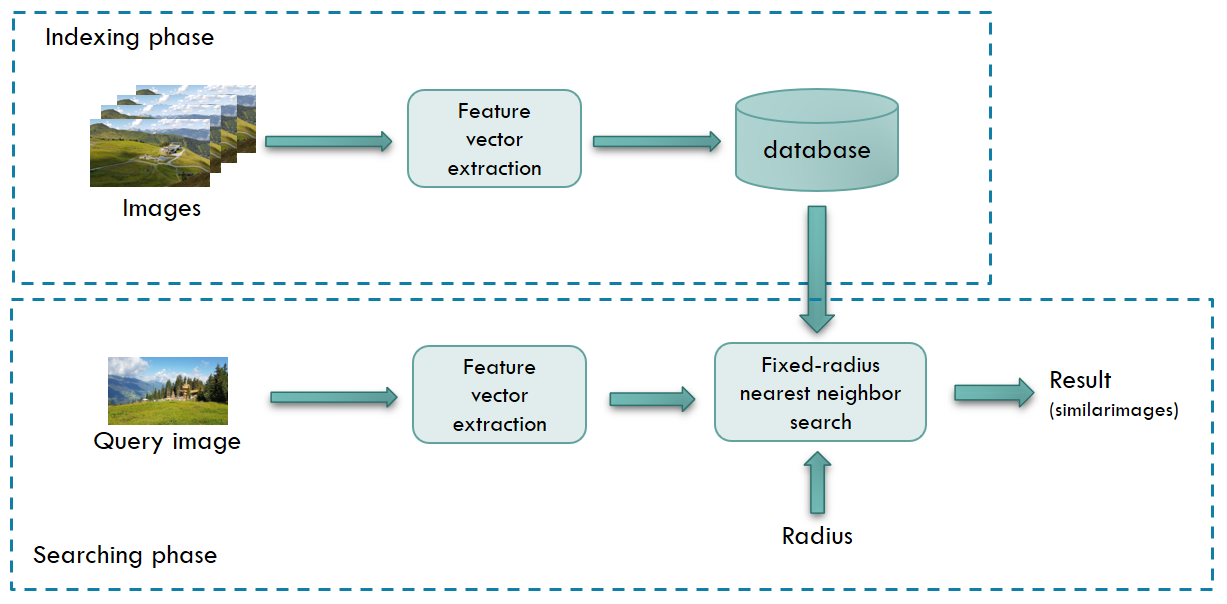
\includegraphics[width=\textwidth]{img/general_ris_framework.png}
	\caption{General framework for Reverse Image Search with fixed-radius nearest neighbor search.}
	\label{fig:general_ris_framework}
\end{figure*}

\subsection{Image representation}
The image representation is usually a $p$-dimensional vector of numerical features or a $q$-bit binary code. The feature vectors should be compact, in order to store millions of them in a database. Many algorithms are able to extract feature vectors from images based on color, texture, shape. We can classify features in two categories: low-level features, which are minor details of the image that are detected by simple algorithms: edges, corners, and so on, and high-level features, which carry more semantic and thus are better understandable by humans: objects, actions, and so on. High-level features are difficult to extract for computers because it is hard to understand the semantic of an image, this is currently an active research field. In the following part, we will describe some algorithms to extract low-level features from images.

A very simple approach is to compute the color histogram of an image. The image representation in this case is a vector of $N$-bins. If there is too much different colors in the image, it is possible to subsample the color space. To compare two histograms, we can use a distance based on correlation.

Color and Edge Directivity Descriptor (CEDD) \cite{chatzichristofis2008cedd} combines, in one histogram, color and texture information. The feature vector size is up to 54 bytes per image. The similarity between two CEDD histograms is measured with Tanimoto coefficient.

Scale-invariant Feature Transform (SIFT) \cite{lowe2004distinctive} extracts distinctive invariant features from images that can be used to perform reliable matching between different views of an object or scene. The features are invariant to image scale and rotation, and are shown to provide robust matching across a substantial range of affine distortion. SIFT detects key points in the image and compute small descriptor for each of them. The number of key points can vary and this is why a feature vector extracted with SIFT does not have a fixed length. To compare two images, their keypoints are matched by identifying their nearest neighbors, which can be very costly dependending on the number of keypoints.

The GIST descriptor was initially proposed in \cite{oliva2001modeling}. It is based on Gabor filters, which measure the orientations and spatial frequencies, and describes a scene with a set of perceptual dimensions (naturalness, openness, roughness, expansion, ruggedness). The GIST description is a feature vector of dimension 960, which can be compared with an Euclidean distance \cite{douze2009evaluation}.

\subsection{Distance}
To compare two image representations one has to choose a distance or similarity function. Depending on the representation many distances are possible.

\subsubsection{$p$-dimensional vectors}
If the image representation is a $p$-dimensional feature vector, following are distances or similarities between $x\in\mathbb{R}^{p}$ and $y\in\mathbb{R}^{p}$.

\textbf{Minkowski distance} is a generalization of Manhattan and Euclidean distances. Euclidean distance can be interpreted as the ordinary straight-line distance between two points in Euclidean space.

\[d_{minkowski}(x, y)=\left(\sum_{i=1}^n |x_i-y_i|^p\right)^{1/p}\]

When $p=1$, the Minkowski distance is equivalent to the Manhattan distance. When $p=2$, it is equivalent to the Euclidean distance. If the function is used to rank vectors according to their distance we can save time by not computing the nth root because this function is monotonically increasing.

\textbf{Cosine similarity} measures the cosine of the angle between two vectors. The cosine similarity is equal to 1 if the angle between vectors is 0. It is equal to 0 if the angle between vectors is $\pi/2$. 

\[s_{cosine}(x, y)=\cos{\theta{}(x, y)}=\frac{x\cdot{}y}{\norm{x}_2\norm{y}_2}\]

\[d_{cosine}(x, y)=\frac{\cos^{-1}s_{cosine}(x, y)}{\pi}\]

For example, the cosine similarity is used in information retrieval. In this field, documents are often represented as vectors containing the number of occurrences of terms. The cosine similarity is meaningful to measure the similarity of two documents regarding their subjects. In facts, what is important is not the number of time a term appears, but whether it appears or not.

Cosine similarity is related to Euclidean distance if the vectors are normalized to unit length.

\[\norm{x-y}^2=(x-y)\cdot{}(x-y)=x\cdot{x}+y\cdot{y}-2x\cdot{y}=\norm{x}^2+\norm{y}^2-2(\norm{x}^2\norm{y}^2\cos{\theta{(x, y)}})\]

Because $\norm{x}=\norm{y}=1$, we can conclude: 

\[\norm{x-y}^2=2(1-\cos{\theta{(x, y)}})\]

\subsubsection{Binary codes}
If the image representation is a $q$-bit binary code, following are distances or similarities between $a\in[0, 1]^{q}$ and $b\in[0, 1]^{q}$.

\textbf{Hamming distance} is the number of positions at which the bits are different. It measures the edit distance between two binary codes if the only allowed operation to transform the code is to flip a bit.

\[d_{hamming}(a, b) = \sum_{i=1}^{n} (a_i \oplus b_i)\]

On computers, this distance is straightforward to compute because it is the number of ones (population count) in the XOR of two binary codes. Since the population count and XOR are two basic operations in modern CPUs, the computation of Hamming distance is very efficient. Following is an implementation in C with two 64-bit binary codes using the POPCOUNT .

\lstset{language=C}
\begin{lstlisting}
int hamming_distance(uint64_t a, uint64_t b)
{
    return __builtin_popcountll(a ^ b);
}
\end{lstlisting}

\textbf{Simple Matching Coefficient} (SMC) is the number of matching bits divided by the length of the binary codes. It is useful when both a value of 0 and 1 for a bit carry equal information. SMC is used for comparing the similarity of two binary codes, to measure a distance one can use the Simple Matching Distance (SMD).

\[SMC=\frac{\text{number of matching bits}}{\text{number of bits}}=\frac{M_{00}+M_{11}}{M_{00}+M_{01}+M_{10}+M_{11}}\]

where:

\begin{description}
\item\textbf{$M_{00}$} is the number of positions where $a$ and $b$ both have a value of 0.
\item\textbf{$M_{01}$} is the number of positions where $a$ has a value of 0 whereas $b$ has a value of 1.
\item\textbf{$M_{10}$} is the number of positions where $a$ has a value of 1 whereas $b$ has a value of 0.
\item\textbf{$M_{11}$} is the number of positions where $a$ and $b$ both have a value of 1.
\end{description}

\[
\begin{split}
SMD & = 1 - SMC \\
    & = 1-\frac{M_{00}+M_{11}}{M_{00}+M_{01}+M_{10}+M_{11}} \\[3ex]
		& = \frac{M_{00}+M_{01}+M_{10}+M_{11}-M_{00}-M_{11}}{M_{00}+M_{01}+M_{10}+M_{11}} \\[3ex]
		& = \frac{M_{01}+M_{10}}{M_{00}+M_{01}+M_{10}+M_{11}}
\end{split}
\]

SMD is related to Hamming distance because $M_{01}+M_{10}$ is equal to the number of positions at which the bits are different, that is the Hamming distance.

\[d_{SMD}(a, b) = \frac{d_{hamming}(a, b)}{q}\]

\textbf{Jaccard Similarity Coefficient} is the number of positions where the two binary codes share a 1 divided by the number of positions where at least one binary codes has a value of 1. To measure a distance, one can use the Jaccard distance. The Jaccard Similarity Coefficient is very similar to the Simple Matching Coefficient, the only difference is that it does not take in account the positions where the two binary codes share a 0. It is useful for asymmetric binary data where a value of 0 and 1 for a bit does not carry equal information, for example a market basket data.

\[J = \frac{M_{11}}{M_{01}+M_{10}+M_{11}}\]

\begin{description}
\item\textbf{$M_{00}$} is the number of positions where $a$ and $b$ both have a value of 0.
\item\textbf{$M_{01}$} is the number of positions where $a$ has a value of 0 whereas $b$ has a value of 1.
\item\textbf{$M_{10}$} is the number of positions where $a$ has a value of 1 whereas $b$ has a value of 0.
\item\textbf{$M_{11}$} is the number of positions where $a$ and $b$ both have a value of 1.
\end{description}

\[d_{Jaccard}(a, b) = 1 - J = \frac{M_{01} + M_{10}}{M_{01}+M_{10}+M_{11}} = \frac{d_{hamming}(a, b)}{q - M_{00}}\]

It is possible to compute the term $M_{00}$ efficiently. It is the number of ones (population count) in $\neg(a \parallel b)$.

\subsection{Nearest Neighbor Search}
Nearest Neighbor Search (NNS) is the problem of finding in a database all the items whose distances to a query item are the smallest. Two variants are interesting for CBIR and RIS: k-nearest neighbors search and fixed-radius near neighbors.

K-nearest neighbors search aims to find the k nearest neighbors of a given query point. Usually the results are ordered by decreasing similarity (i.e. increasing distance). When applied to CBIR it is interesting in order to explore an image collection, because if the first results are not interesting, one can just look at the following results. 

Fixed-radius near neighbors aims to find all points that are within a radius of a given query point. Even if it is possible to sort the results according to the distance, the results should be considered as a set of unranked images. When applied to CBIR, this method is interesting for identifying content because only relevant images are returned, thus the result is composed of a varying number of images. The determination of an adequate radius, in accordance with the actual application, is critical. Information retrieval research has shown that precision and recall follow an inverse relationship \cite{datta2008image}. If the radius is too low, the precision is better at the expense of the recall, and vice versa. Depending on the application, one can want to favor precision, to authenticate content because there is fewer false-positives, or recall, to identify content because the user can deal with false positives.

Suppose our dataset is composed of $p$-dimensional feature vectors in a Euclidean space $D\equiv{\{x_i\}}_{i=1}^{n}$ where $x_i\in\mathbb{R}^{p}$. Let $z\in\mathbb{R}^{p}$ be a query feature vector, the one-nearest neighbor of the query $z$ is defined as:

\[KNN_{1}(z)=\argmin_{1 \leq i \leq n} \norm{z-x_i}^2\]

Let $r\in\mathbb{R}^+$ be a radius, the fixed-radius nearest neighbors of the query $z$ are defined as:

\[FRNN_{r}(z)=\{y \in D \;|\; \norm{y - z} \leq r\}\]

For $p$-dimensional feature vectors, there exist algorithms for exact nearest neighbor search such as the k-d tree, R-tree or MVP tree. But unfortunately, because of the curse of dimensionality, they are not efficient for high dimensional data (more than 20 dimensions). For this reason, Approximate Nearest Neighbor Search (ANNS) is gaining more interest because it allows for faster searching time with only small actual errors. In any case, we can refine a list of approximate nearest neighbors by pruning the items with the actual distance on the original features. The Locality Sensitive Hashing (LSH) framework is one approach to Approximate Nearest Neighbor Search and is detailed later in this part.
\chapter{Perceptual Hashing}

\label{chapter:PerceptualHashing}

% ----------------

\section{Definition}
A perceptual hash function is a type of hash function that has the property to return analogous outputs if inputs are similar. This allows one to make meaningful comparisons between hashes in order to measure the similarity between the source data. The definition of a hash function according to \cite{menezes1996handbook} is: 

\begin{quote}
A hash function is a computationally efficient function mapping binary strings of arbitrary length to binary strings of some fixed length, called hash-values.
\end{quote}

In the case of a perceptual hash function, four more properties should be present according to \cite{zauner2010implementation}:

\begin{quote}
Let $H$ denote a hash function which takes one media object (e.g. an image) as input and produces a binary string of length $l$. Let $x$ denote a particular media object and $\widetilde{x}$ denote a modified version of this media object which is "perceptually similar" to $x$. Let $y$ denote a media object that is "perceptually different" from $x$. Let $x'$ and $y'$ denote hash values. ${0,1}^l$ represents binary strings of length $l$. Then the four desirable properties of a perceptual hash are identified as follows.

A uniform distribution of hash-values; the hash-value should be unpredictable.
\[\mathbb{P}(H(x)=x') \approx \frac{1}{2^l}  \quad  \forall x' \in \{0, 1\}^l\]

Pairwise independence for perceptually different media objects.
\[\mathbb{P}(H(x)=x' | H(y)=y') \approx \mathbb{P}(H(x)=x') \quad \forall x', y' \in \{0, 1\}^l\]

Invariance for perceptually similar media objects.
\[\mathbb{P}(H(x)=H(\widetilde{x})) \approx 1\]

Distinction of perceptually different media objects. It should be impossible to construct a perceptually different media object that has the same hash-value as another media object.
\[\mathbb{P}(H(x)=H(y)) \approx 0\]

\end{quote}

Most of the time, to achieve these properties, the perceptual hash function extracts some features of media objects that are invariant under slight modifications. For example, knowing how a compression algorithm works, it is possible to find some invariant features and then design a perceptual hash based on them. Some examples of perceptual hash functions for images are detailed later in this section.

\section{Usage}
Perceptual hash functions can be used in the context of CBIR or RIS for representing images but they are also useful in other contexts. Due to the properties inherited from the hash functions they can be used to authenticate media objects even if they are slightly modified, for example lossy compressed. The image creator can generate a perceptual hash from his original work. Then, as explained in \cite{zauner2010implementation}, he has two options. 

On the one hand it is possible to sign the perceptual hash with a private key in order to have a digital signature that is robust to slight modifications, for example JPEG compression. This measure protects the receiver of the media object because he can check its authenticity.

On the other hand, it is possible to use the perceptual hash for digital watermarking. This measure protects the content author. For example, a different watermark can be applied on different images. Then if an illegal copy is found the copyright owner can infer who is responsible for the data leak. 

\section{Implementations}
In this section, we present the three examples of implementations of perceptual hash functions, which take images and output binary codes, from \cite{zauner2010implementation}.

The Discrete Cosine Transformation (DCT) based perceptual hash function takes advantage of the property that low-frequency DCT coefficients are mostly stable under image modifications to construct a 64 bits binary code, which are compared with a Hamming distance. See our implementation in appendix \ref{chapter:ImplementationDCTPerceptualHash}

The Marr-Hildreth (MH) operator, also denoted as the Laplacian of Gaussian (LoG), is a special case of a discrete Laplace filter. It is an edge and contour detection based image feature extractor. The MH operator generates vectors encoded on 576 bits.

The Radial Variance hash is based on the Radon transform that is the integral transform which consists of the integral of a function over a straight line. It is robust against various image processing steps (e.g. compression) and more robust than the DCT and MH based perceptual hash functions against geometrical transformations (e.g. rotation up to 2 degrees).

\chapter{Convolutional Neural Networks}

\label{chapter:ConvolutionalNeuralNetworks}

% ----------------

\section{Definition}
A Convolutional Neural Network (CNN) is a class of feed-forward neural network. CNN are mainly applied in the fields of computer vision and natural language processing. It has been first presented in \cite{lecun1998gradient}. Recent progresses have led to a gain in interest in this method and also in a broader field called Deep Learning, which is described in \cite{lecun2015deep}. This section is mainly based on this latter article. It has been a great discover because this class of network is able to automatically learn the features to extract from a dataset. Whereas traditionally, the previous works in computer vision were based on hand-engineered features. This difference is essential because the key success factor of CNN is the amount of data and computation power available instead of field knowledge.

CNN are inspired by our visual cortex, in particular, the connectivity pattern between layers of artificial neurons is restricted to a region as it is in our visual system with receptive fields. With this special connectivity pattern, CNN take advantage of natural signals, which are often locally highly correlated. Another property of natural signals is the fact that the local statistics of images are invariant to location. If a motif can appear in one location of an image, it could also appear somewhere else.

CNN are built on top of four key ideas: local connection, shared weights, pooling and use of many layers. The architecture of a typical CNN is composed of these layers; in a first part: convolution layer, ReLU, pooling layer and in a second part: fully connected layer, loss layer.

The convolution layer applies a set of discrete convolutions on the output of the previous layer. Each convolution is done using a kernel (also called: mask, filter bank) and produces a 2D feature map. The feature maps contain high activations if their convolutions have detected an interesting motif. The layer's parameters are the weights in the kernels. This layer can also be seen as a layer with local connections, so that a neuron is only connected to neurons of the previous layer in the same region. Local connections give the ability to the layer to detect local patterns from the previous layer. Moreover, the weights of the local connections are shared among all neurons in the layer, this means that the same local pattern can be detected in the same way anywhere in the previous layer.

\begin{figure*}
	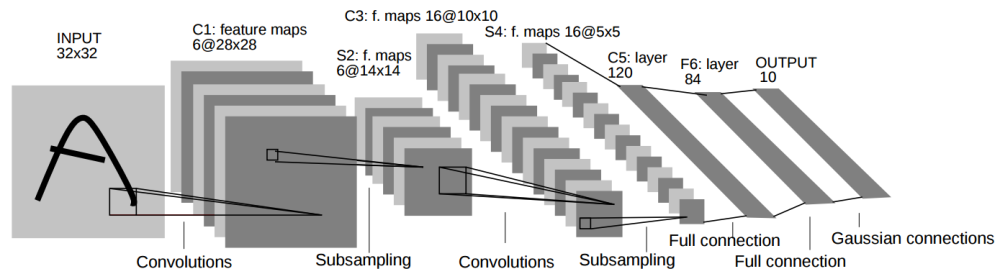
\includegraphics[width=\textwidth]{img/cnn.png}
	\caption{Architecture of LeNet-5, a basic Convolutional Neural Network}
	\label{fig:cnn}
\end{figure*}

The ReLU (Rectified Linear Units) applies a non-linear function $f(x) = \max(0, x)$ to the output of the previous convolution layer. Other non-linear activation function are available: hyperbolic tangent or sigmoid function for example. The ReLU is the most common because the training of the neural network is faster with it \cite{krizhevsky2012imagenet}.

The pooling layer splits the output of the previous layer into a grid, then on each cell of the grid a pooling function is applied and outputs only a single value. Thus, the pooling layer is a down-sampling step, the resolution of the grid can vary and affects the sampling rate. This layer merges multiple semantically similar features into one. Due to the down-sampling, the position of the feature is not accurately preserved, therefore an invariance to small shifts or distortions is spawned. In fact, the position of a feature is not as important as its relative position to others features. A typical pooling function outputs the maximum value of a local patch.

Repeating these layers several times in this order: convolution, ReLU, pooling, one can exploit the fact that high level features are composed of lower level features. The first group of layers can detect small details such as edges and contours. The second layer can detect higher level features such as motifs, and so on. This process is repeated so that firstly, edges are merged into motifs, motifs into parts and finally parts into objects. The architecture of a very basic CNN is shown in figure \ref{fig:cnn}.

After this first part composed of convolution layers, ReLU, pooling layers, a second part of the neural network is composed of fully-connected layers and a loss layer. This second part is a classical feed-forward neural network used to classify the features coming from the first part. The training of CNN is possible using the backpropagation algorithm. Because of the local connectivity and the shared weights, there is less parameters in the model thus the network is less prone to overfitting and generalizes better.

\section{Usage}
Convolutional neural networks are mostly used in supervised learning for classification tasks. One of the first successful commercial application was to recognise handwritten digits on bank checks \cite{lecun1998gradient}. In this task, the system is given a normalized, grayscale, 28-by-28 pixels image of a digit and outputs the class of the image: zero, one, two, and so on until nine. The same technique can be used for Optical Character Recognition (OCR). By using a sliding window on an image, it is possible to use a CNN to recognize if a face is depicted at a certain position \cite{garcia2004convolutional}. It is possible to use CNN for image classification \cite{krizhevsky2012imagenet}, for example the ImageNet dataset is composed of roughly 1.2 million images divided into 1,000 classes, the goal being to predict the class of a given image. Scene labeling consists in labeling each pixel in an image with the category of the object it belongs to. CNN have been successfully applied to this task \cite{farabet2013learning}. It is useful for example to self-driving cars and more generally to autonomous robots. When used with one dimensional convolution, CNN are able to process acoustic signals for automatic speech recognition \cite{sercu2015verydeep}.

\section{Feature extraction}
Recent work showed that the representation learned by the CNN is a good descriptor for image retrieval. With the AlexNet network \cite{krizhevsky2012imagenet}, one can use the feature activations induced by an image at the last hidden layer to represent an image. Experiments has shown that semantically similar images get a similar feature vector in a Euclidean space, even if the images are not close in L2. The only drawback is that the representation is a real-valued vector of dimension 4096. Therefore, the computation of the distance between two vectors is expensive, moreover the storage cost could also be an issue. To tackle this issue, the authors suggest a dimensionality reduction with an auto encoder.

In a later paper \cite{babenko2014neural}, the performance of feature vectors extracted with CNN in the context of image retrieval is studied more in depth. The conclusion is that CNN performs well for image retrieval, even if the network is trained on an unrelated classification task. The performances can be improved with a fine tuning on a dataset similar to the retrieval dataset. For example, by using a neural network trained on ImageNet to retrieve landscape images, the performances are good. Unsurprisingly, after a retraining on a dataset composed of landscape images the performances become even better. The compression with PCA is also investigated, and the retrieval performance is not too much affected when compared to other state of the art descriptors. Image features extraction with CNN, for all these reasons, seems to be very promising for image retrieval.

\section{Models}
\label{chapter:ConvolutionalNeuralNetworks:section:Models}
In this section, three models used for the ImageNet Large Scale Visual Recognition Challenge (ILSVRC) are presented. All of them are implemented in the Keras \cite{chollet2015keras} library and are used later in this thesis.

The VGG network \cite{simonyan2014verydeep} was created in 2014 for ILSVRC. The authors investigated the effect of depth on the accuracy. For that purpose, they use a simple convolutional neural network with very small (3x3) convolution filters with stride and pad of 1, 2x2 maxpooling with stride 2, and push the depth to 16-19 layers, which was a lot at the time. VGG16 and VGG19 are detailed in table \ref{table:vgg_model}.

\begin{table}[h]
\centering
\caption{Configurations of VGG16 and VGG19 networks. The convolutional layer parameters are denoted as "`conv(receptive field size)-(number of channels)"'. The ReLU activation is not shown for brevity.}
\label{table:vgg_model}
\begin{tabular}{|c|c|}
\hline
VGG16                     & VGG19                     \\
\hline
\multicolumn{2}{|c|}{input (224x224 RBG image)}       \\
\hline
conv3-64                  & conv3-64                  \\
conv3-64                  & conv3-64                  \\
\hline
\multicolumn{2}{|c|}{maxpool}                         \\
\hline
conv3-128                 & conv3-128                 \\
conv3-128                 & conv3-128                 \\
\hline
\multicolumn{2}{|c|}{maxpool}                         \\
\hline
conv3-256                 & conv3-256                 \\
conv3-256                 & conv3-256                 \\
\textbf{conv3-256}        & conv3-256                 \\
                          & \textbf{conv3-256}        \\
\hline
\multicolumn{2}{|c|}{maxpool}                         \\
\hline
conv3-512                 & conv3-512                 \\
conv3-512                 & conv3-512                 \\
\textbf{conv3-512}        & conv3-512                 \\
                          & \textbf{conv3-512}        \\
\hline
\multicolumn{2}{|c|}{maxpool}                         \\
\hline
conv3-512                 & conv3-512                 \\
conv3-512                 & conv3-512                 \\
\textbf{conv3-512}        & conv3-512                 \\
                          & \textbf{conv3-512}        \\
\hline
\multicolumn{2}{|c|}{maxpool}                         \\
\hline
\multicolumn{2}{|c|}{FC-4096}                         \\
\hline
\multicolumn{2}{|c|}{FC-4096}                         \\
\hline
\multicolumn{2}{|c|}{FC-1000}                         \\
\hline
\multicolumn{2}{|c|}{soft-max}                        \\
\hline
\end{tabular}
\end{table}

The InceptionV3 network \cite{szegedy2015rethinking} was created in 2015. Instead of stacking convolutional and pooling layers sequentially on top of each others, some layers are in parallel and their results are merged periodically. As shown in figure \ref{fig:inceptionv3} from Google Research Blog \footnote{https://research.googleblog.com/2016/03/train-your-own-image-classifier-with.html}, the key idea of this network is to stack Inception modules, which are composed of convolutional and pooling layers. This can be easily seen in figure \ref{fig:inceptionv3}. By using fewer weights than previous neural networks, for instance about 30x fewer parameters than VGG19, the computational cost of InceptionV3 is suitable for big-data or mobile scenarios.

\begin{figure}[h]
	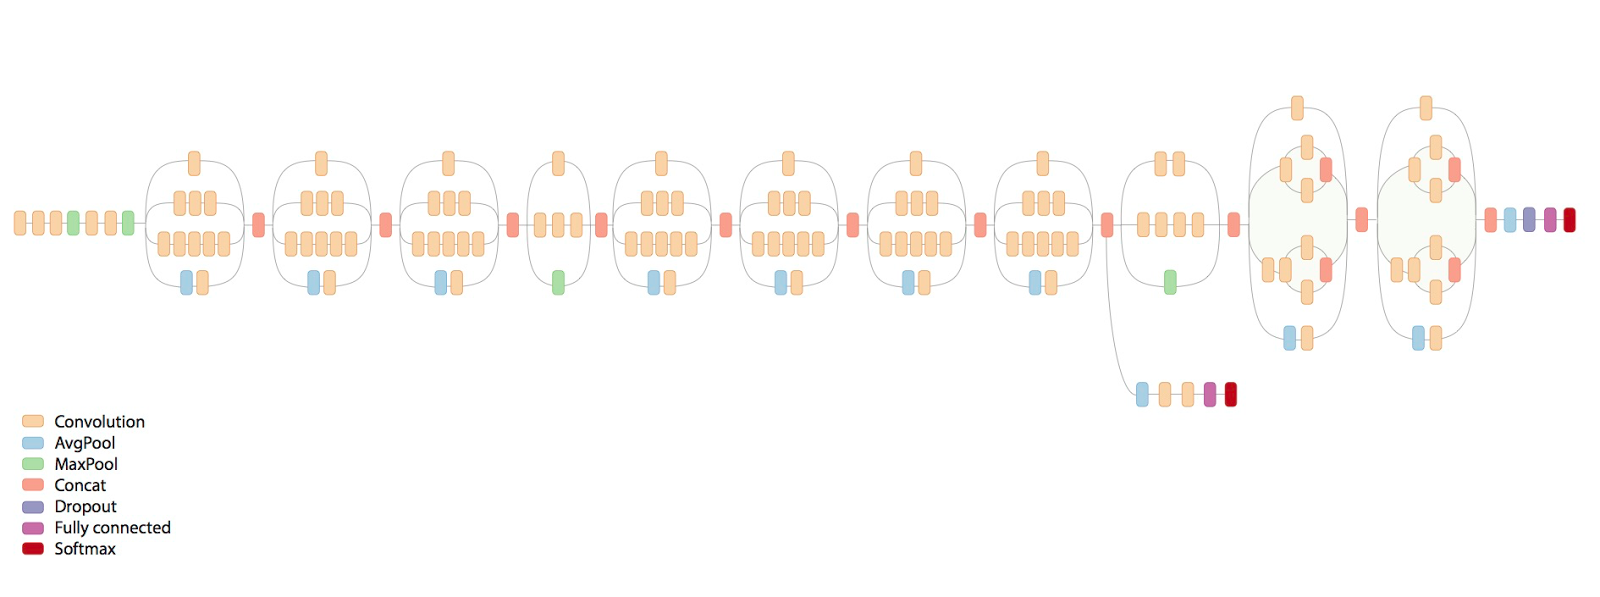
\includegraphics[width=\textwidth]{img/inceptionv3.png}
	\caption{Architecture of the InceptionV3 network.}
	\label{fig:inceptionv3}
\end{figure}

The ResNet50 network \cite{kaiming2015deepresidual} was created in 2015 for ILSVRC. The authors use a 50 layers Residual Network, whose key idea is to introduce shortcuts connections into a sequential network. As networks are becoming deeper, the learning is more difficult because of the vanishing/exploding gradient problem. In particular, with the network depth increasing, accuracy gets saturated and then degrades rapidly. The idea behind shortcuts in Residual Networks is to by-pass a set of layers if they are not useful to improve the accuracy of the whole network. Thus, in theory, it is possible to stack as many building blocks as possible without affecting the accuracy, because unnecessary blocks can be skipped. Figure \ref{fig:renet50} shows a Residual Network with 34 layers

\begin{figure}[p]
	\centering
	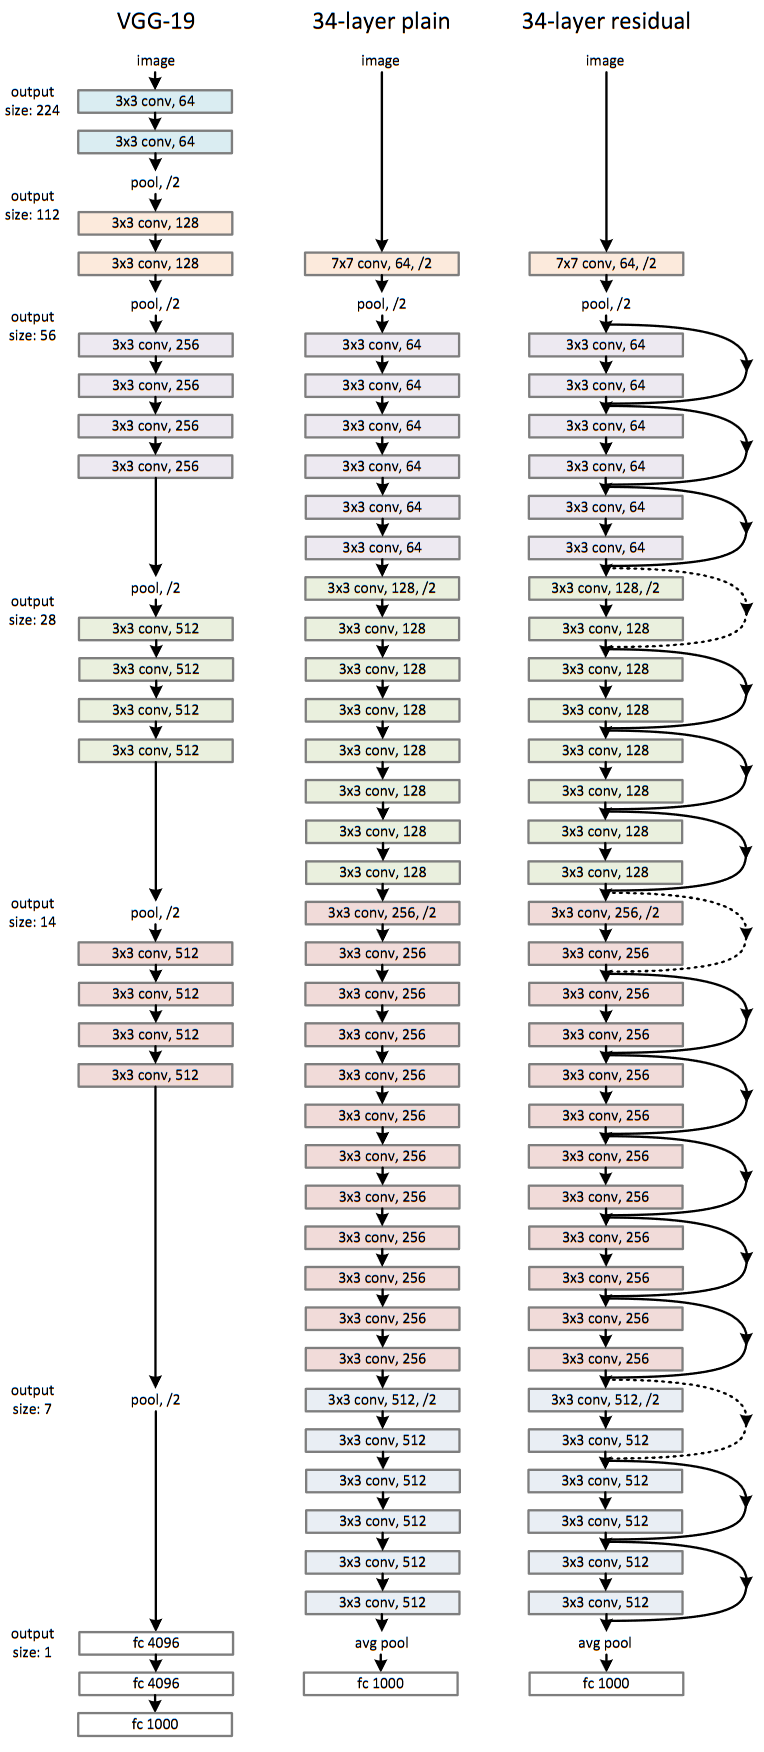
\includegraphics[height=0.9\textheight]{img/resnet34.png}
	\caption{\textbf{Left}: the VGG19 model as a reference. \textbf{Middle}: a plain network with 34 parameters layers. \textbf{Right}: a Residual Network with 34 parameter layers. The dotted shorcuts increase dimensions.}
	\label{fig:renet50}
\end{figure}

\chapter{Hashing for Dimensionality Reduction}

\label{chapter:HashingDimensionalityReduction}

% ----------------

\section{Hashing into binary codes}
As detailed in chapter \ref{chapter:PerceptualHashing}, images can be represented with small binary codes (also known as hash codes), which can be compared with a Hamming distance. Because binary codes are small and easy to handle on computers, millions of them can be stored in a database. Furthermore, the whole database can fit in memory, which leads to less IO operations. As explained in chapter \ref{chapter:ReverseImageSearch}, the Hamming distance can be computed very quickly even on commodity hardware thanks to the POPCOUNT instruction.

To extract a representation of an image in the form of a binary code, we can use a perceptual hash function. Formally a perceptual hash function maps high-dimensional inputs $x\in\mathbb{R}^{p}$, into binary codes, $y\in\mathbb{H}\equiv\{0, 1\}^{q}$, and is defined as: $y=h(x)$. A suitable hash function should map similar (resp. dissimilar) images into similar (resp. dissimilar) binary codes according to a selected distance.

In the next two sections, we review several methods classified in two categories: data independent approaches, which make no prior assumption about the data distribution, and machine learning approaches, which take advantage of the data distribution to optimize the hash function. For each method we will describe the hash function and its associated similarity measure. The hash function determines the partitioning of the input space, which is important to consider. A linear hash function might have more difficulties to preserve similarities of a data set when compared to a non-linear hash function. Non-linear hash functions can more finely discriminate points that are not linearly separable. Moreover non-linear hash functions can discover the internal model of the input space to be able to represent it in a more efficient manner. Hence the binary codes can be shorter without necessarily being less efficient.

There exist different types of hash function: linear transformations, which will be described later, linear transformations followed by a cosine transform, functions based on kernels, functions based on multilayer neural networks, and so on.

One popular hash function is a linear transformation $h_W(x)=thr(Wx)$ where $W\in\mathbb{R}^{q\times{}p}$ and $thr(\cdot)$ is an element-wise Heaviside function. Figure \ref{fig:lsh} shows the partitioning of the space for this particular function. Each row of $W$ denotes the normal of a hyperplane in the input space and determines the value of one bit; 1 is assigned to points on one side of the hyperplane and 0 to points on the other side.

\begin{figure}
	\centering
	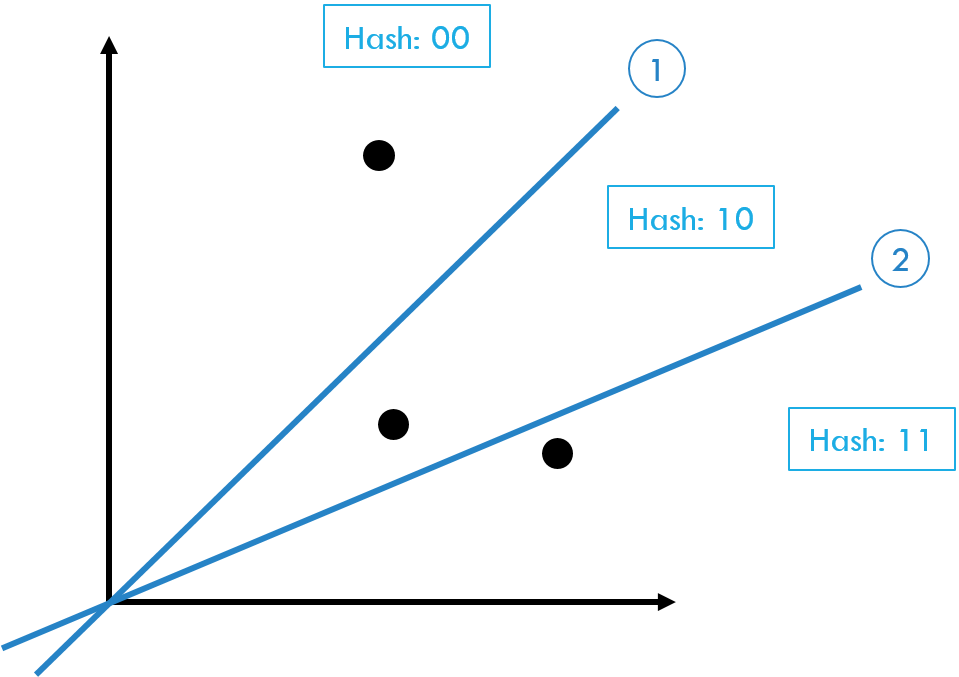
\includegraphics[height=0.3\textheight]{img/lsh.png}
	\caption{Partitioning of the space for a hash function based on a linear transformation}
	\label{fig:lsh}
\end{figure}

The most popular similarity measure is based on Hamming distance. Other options are possible: Weighted Hamming distance, Jaccard coefficient, precomputed lookup table, and so on.

Depending on the application and the dimensionality of the inputs and outputs, the complexity of the computation of a hash function can be unacceptable. For example, the computation of $q$-bit binary codes for a $p$-dimensional input using a linear transform has a complexity of $O(qp)$. More expressive hash functions can have a higher complexity. Thus, it is important to carefully select the hash function according to the application.

\section{Data independent approaches}
In this section, we present the data independent approaches, which makes no prior assumption about the data distribution. The most popular approach is based on Locality Sensitive Hashing (LSH) \cite{wang2014hashing}. The general idea of LSH is to hash similar input items to the same binary code with higher probability than dissimilar input items. In other words, the goal of LSH is to maximize collisions rather than to avoid them. LSH comes with theoretical guarantees that a specific metric is increasingly well-preserved as the code length increases.

There are different LSH schemes that can preserve different distances: $l_p$ distance, angular distance, Hamming distance, and so on. We will present LSH with random projection which preserves the angular distance.

\subsection{Random projection}
Locality Sensitive Hashing based on random projection \cite{charikar2002similarity} is designed for the angular distance. Thus, it preserves the cosine similarity. The angular distance between two vectors can be computed with

\[s_{cosine}(x, y)=\cos{\theta{}(x, y)}=\frac{x\cdot{}y}{\norm{x}_2\norm{y}_2}\]

\[d_{cosine}(x, y)=\frac{\cos^{-1}s_{cosine}(x, y)}{\pi}\]

The hash function is defined as $h_W(x)=thr(Wx)$. Each coefficient of W is randomly chosen from a Gaussian distribution. Then the probability of collision is 

\[\mathbb{P}(h_W(x)=h_W(y))=1-distance=1-\frac{\theta{}(x, y)}{\pi}\]

It is possible to choose the length of binary codes according to the number of input vectors to hash. According to \cite{wang2014hashing}, for $n$ vectors, take $O(\log^2{n})$.

\section{Machine Learning approaches}
In this section, we present the machine learning approach, which takes advantage of the data distribution to optimize the hash function. Two different approaches are detailed, Semantic Hashing is based on an autoencoder, Minimal Loss Hashing and Triplet Loss Ranking, are based on the minimization of a loss function.

In addition to the two main components, hash function and similarity measure, machine learning solutions have an optimization criterion, which defines the objective that the algorithm pursue. A basic optimization criterion is the order-preserving criterion where the results of the ANN search are compared to an external reference. The similarity alignment criterion minimizes the difference between the similarities computed in output and input space. The coding consistent criterion encourages similar (resp. dissimilar) codes when the inputs are similar (resp. dissimilar) and penalizes dissimilar (resp. similar) codes when the inputs are similar (resp. dissimilar). The coding balance criterion aims to uniformly distribute the input vectors among the hash buckets.

In approaches based on machine learning, the parameters of the hash function are optimized using the input data. As usually in machine learning, it is possible to learn the model on a training data set and then use it with other data. A better way to proceed is to use all data to train the model. In this case, over-fitting is not an issue because there is no need to generalize to new data.

While presenting the approaches, we only consider the hash function, the similarity measure and the optimization criterion, without spending too much time on the learning algorithm, assuming that a good solution is found.

\subsection{Semantic Hashing}
Semantic Hashing \cite{salakhutdinov2007semantic},\cite{salakhutdinov2009semantic} is an unsupervised learning approach based on Neural Networks, in fact no similarity information is used. A multilayer autoencoder is used to discover a lower dimensional representation of the input vectors. Its architecture is shown in figure \ref{fig:auto_encoder}. The code layer, which is in the middle of the autoencoder, is forced to use a small number of binary variables (e.g. 32). The model is first pretrained as a stack of RBM's, then it is unrolled to create a multilayer autoencoder, which is fine-tuned by minimizing the root mean squared reconstruction error with backpropagation. To get the final binary code, the activations of the units in the code layer are simply thresholded.

With this framework, semantically similar documents are mapped to similar binary codes. Thus, we can use a Hamming distance to compare two binary codes. To perform an approximate nearest neighbor search, rather small codes (e.g. 20 bits) are used and a hash table lookup method is performed with a small radius (e.g. 4 bits). To improve the precision, it is possible to use a two-stage method. At first, a list of candidates is obtained with 28 bits codes, it is then pruned with 256 bits codes. For the code layer, two technical solutions are available.

On the one hand, logistic units are trained with deterministic Gaussian noise. The noise doesn't change during the training, and because there are more examples than parameters in the model, it is forced to generalize rather than to tailor the parameters to the beforehand fixed noise. The presence of noise forces the input of the activation function to be large and negative for some training cases and large and positive for others. Consequently, the noise has only a small impact on the output of the layer.

On the other hand, an easier approach discovered later \cite{krizhevsky2011using}. Instead of logistic units, binary stochastic units are used in the code layer and no noise is added. A binary stochastic unit outputs either 1 or 0 otherwise depending on a probability given by a logistic function.

\[z_i=b_i+\sum\nolimits_{j}s_{i}w_{ij}\]
\begin{align*}
\mathbb{P}(s_i=1)=\frac{1}{1+\textrm{e}^{-z_i}} && \mathbb{P}(s_i=0)=1-\mathbb{P}(s_i=1)
\end{align*}

To train a binary stochastic unit we pretend during the backpropagation, that the output value comes from a normal logistic unit and it gives a smooth gradient for the backpropagation.

\begin{figure}
	\centering
	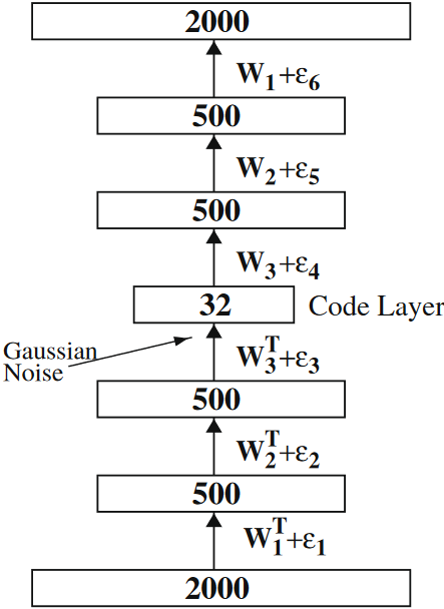
\includegraphics[height=0.3\textheight]{img/auto_encoder.png}
	\caption{Autoencoder in Semantic Hashing}
	\label{fig:auto_encoder}
\end{figure}

\subsection{Minimal Loss Hashing}
Minimal Loss Hashing (MLH) \cite{norouzi2011minimal},\cite{norouzi2016} is a supervised approach based on a hinge-like loss function. A linear hash function is used $h_W(x)=thr(Wx)$, it is also possible to use it with other hash functions as long as they are differentiable with respect to their parameters, so that we can compute the Jacobian. The Hamming distance is used to compare the output binary codes.

The learning is based on a training data set of labeled pairs $(x_i, x'_i, s_i)$ where $x_i$ and $x'_i$ are $p$-dimensional centered training points and $s_i$ is a similarity label, whose value is 1 if $x_i$ and $x'_i$ are similar and 0 if dissimilar. To preserve a specific metric one can compute the similarity label by thresholding the pairwise distance. Alternatively, to preserve the semantic similarity, one can assign a similarity label based on the class label.

For each sample in the training data set, a loss function $l_{pair}: \{0, 1\}^{q}\times\{0, 1\}^{q}\times\{0, 1\}\rightarrow\mathbb{R}^{+}$ assesses the quality of the mapping by assigning a cost to a pair of binary codes and a similarity label. By minimizing the loss over all training examples, we can learn the parameters of the hash function.

\[L(w)=\sum\limits_{i=1}^n l_{pair}(h_W(x_i), h_W(x'_i), s_i)\]

To optimize the parameters of the hash function, the key point of MLH is to use a coding consistent criterion based on a hinge-like loss function. A hyper-parameter $\rho$ is a threshold of distance in Hamming space, that defines the boundary between similar and dissimilar codes. If the distance between two codes is less than (resp. more than) $\rho$ we can consider them as similar (resp. dissimilar). In addition, the $\lambda$ parameter adjusts the penalty incurred for dissimilar pairs when they are too close in comparison to the penalty incurred for similar pairs when they are too far from each other. Although it is a slow process, a good value for these hyper parameters can be found with a validation set. Let $\norm{h - h'}_{H}$ be the Hamming distance between binary codes $h$ and $h'$. The pairwise loss based on the hinge function is defined as:

\[
	l_{hinge}(h, h', s)=
	\begin{cases}
	\max(\norm{h - h'}_{H} - \rho + 1, 0) & \text{for } s=1 \\
	\lambda\max(\rho - \norm{h - h'}_{H} + 1, 0) & \text{for } s=0
	\end{cases}
\]

Minimal Loss Hashing builds a convex-concave upper bound on it. Then a stochastic gradient-based approach is used to minimize the loss function. The learning algorithm is online, scales well to large data sets and large code lengths.

\subsection{Triplet Ranking Loss}
Triplet Ranking Loss (TRL) \cite{norouzi2012hamming},\cite{norouzi2016} is a supervised approach that generalizes Minimal Loss Hashing. While certainly good at learning a metric structure (e.g. Euclidean, Cosine) of the input data, the goal of this approach is rather to preserve the semantic similarity. When no pairwise similarity is available, one could rely on a generic distance (e.g. Euclidean) but this often produce unsatisfactory results. TRL, on the other hand, is based on the relative similarity between a triplet of points. Thus, no pairwise similarity label is required.

A linear hash function is used $h_W(x)=thr(Wx)$, as with MLH it is possible to use other hash functions as long as they are differentiable with respect to their parameters. The Hamming distance is used to compare the output binary codes.

The learning is based on a training data set of triplets of $p$-dimensional centered training points $(x, x^{+}, x^{-})$ such that the pair $(x, x^{+})$ is more similar than the pair $(x, x^{-})$. To build a training data set that preserves semantic similarity one can pick two points from the same class and one point from another class.

As with MLH, for each sample in the training data set, a loss function $l_{rank}: \{0, 1\}^{q}\times\{0, 1\}^{q}\times\{0, 1\}^{q}$ assesses the quality of the mapping by assigning a cost to a triplet of binary codes. The loss function should penalize the examples where $h_W(x_i)$ is closer to $h_W(x^{-}_i)$ than to $h_W(x^{+}_i)$ in Hamming distance. By minimizing the loss over all training examples, we can learn the parameters of the hash function.

\[L(w)=\sum\limits_{i=1}^n l_{rank}(h_W(x_i), h_W(x^{+}_i), h_W(x^{-}_i))\]

To optimize the parameters of the hash function, TRL uses a hinge-like loss function. On the contrary of MLH, there is no hyper parameter, which makes the learning easier because there is no need to find them a good value with a validation set. The loss is zero when $h_W(x_i)$ is closer to $h_W(x^{+}_i)$ than to $h_W(x^{-}_i)$ in Hamming distance. Let $\norm{h - h'}_{H}$ be the Hamming distance between binary codes $h$ and $h'$. In this case, the loss is zero when $\norm{h - h^{+}}_{H}$ is at least one bit smaller than $\norm{h - h^{-}}_{H}$. The triplet loss based on the hinge function is defined as:

\[
	l_{rank}(h, h^{+}, h^{-})=\max(\norm{h - h^{+}}_{H} - \norm{h - h^{-}}_{H} + 1, 0)
\]

The same optimization technique as MLH is used. A convex-concave upper bound is built on the loss function. Then a stochastic gradient-based approach is used to minimize the loss function. TRL is more flexible than the pairwise hinge loss and is shown to produce superior hash functions. A simple kNN classifier on the learned binary codes is competitive with state-of-the-art classifiers on CIFAR and MNIST.

\section{Comparison}
In this section, we compare the methods in term of hash functions, partitioning of the input space and retrieval performance. We don't take in account the optimization technique of the machine learning approaches, assuming that a good solution is found.

Fundamentally, data independent approaches should be less efficient than machine learning approaches because they don't take in account the data distribution. This means that on the same instance, depending on the data distribution, the machine learning solutions should generally yield better results. The binary codes generated by data independent approaches should be longer than their equivalent from machine learning approaches for the same retrieval accuracy. The data independent solutions are nevertheless more general and come with theoretical guarantees that a specific metric is increasingly well preserved as the code length increases. Moreover, one has to be very careful when training a machine learning approach because there is many pitfalls: trying to generalize from a bad sampled training data set, making an error during the preprocessing, choosing wrong values for the hyper parameters, choosing, a priori, a hash function that is not appropriate, training only one model and not benchmarking it against other approaches, and so on.

\begin{figure*}
	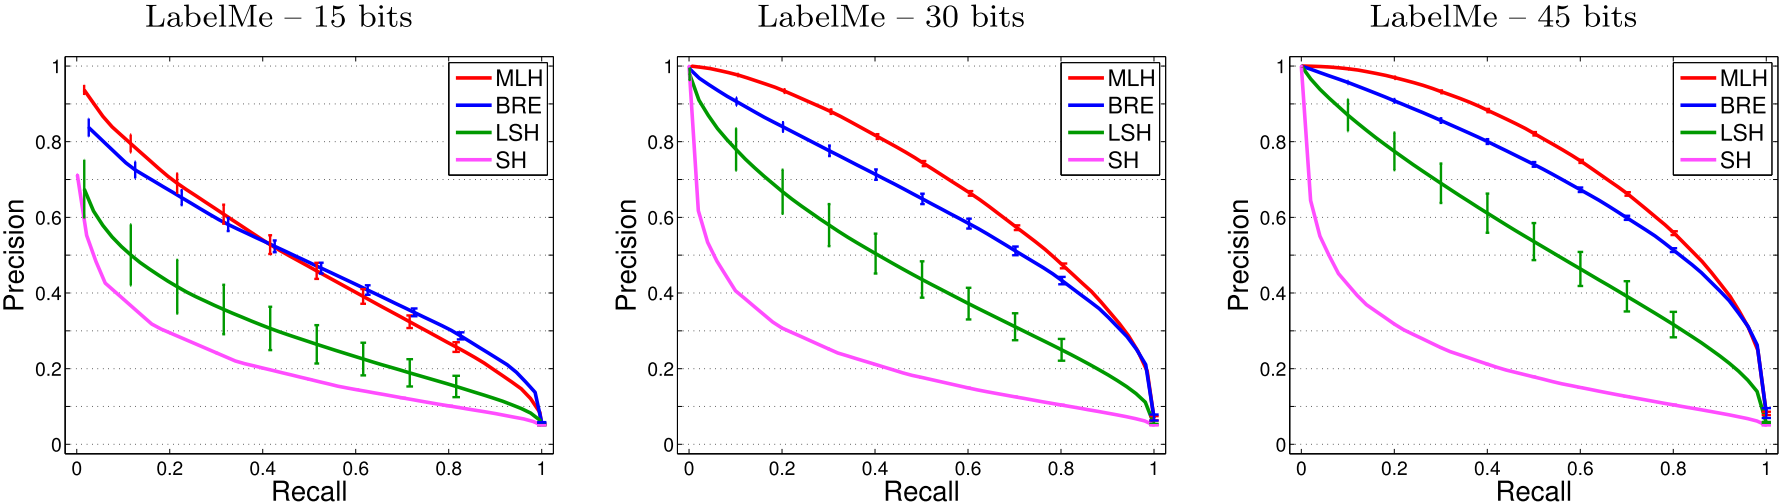
\includegraphics[width=\textwidth]{img/mlh_labelme.png}
	\caption{Precision-recall curves on LabelMe for different methods for different code lengths. \cite{norouzi2011minimal}}
	\label{fig:mlh_labelme}
	
	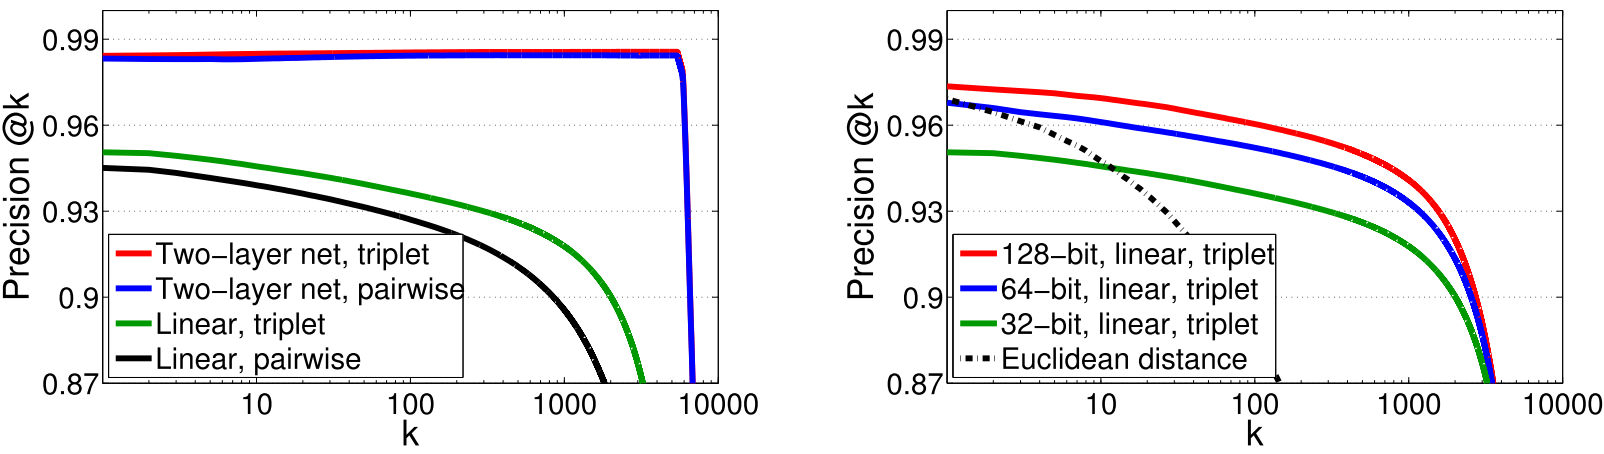
\includegraphics[width=\textwidth]{img/trl_vs_mlh.png}
	\caption{MNIST precision@k: (left) four methods with 32-bit codes; (right) three code lengths with triplet loss. \cite{norouzi2012hamming}}
	\label{fig:trl_vs_mlh}
\end{figure*}

Based on experiments conducted by the authors of the approaches we can have an idea on their relative performances.

A first experiment, conducted by the authors of Minimal Loss Hashing (MLH) \cite{norouzi2011minimal}, compares it with LSH and other methods. Six data sets are used: \textit{Photo-tourism}, a collection of images represented as 128D SIFT features, \textit{LabelMe} and \textit{Peekaboom}, collections of images represented as 512D Gist descriptors. \textit{MNIST}, a collection of 784D grayscale images of handwritten digits, \textit{Nursery} with 8D features, a synthetic data set comprising uniformly sampled points from a 10D hypercube. All methods used identical training and test sets. The similarity labels are based on a thresholded Euclidean distance so that each point has, on average, 50 neighbors. On each data set, input vectors are mean-centered. On all but the 10D Uniform data set, each datum is normalized. Some methods improve with dimensionality reduction so a PCA is applied to retain 40 dimensions (except for 10D Uniform and 8D Nursery). Average and standard deviation of precision/recall are computed on 10 executions of all methods, except for Spectral Hashing (SH). In this review we only present the precision-recall curves on LabelMe for different code lengths, in figure \ref{fig:mlh_labelme}. Other experiments are conducted in the original paper: precision using a Hamming radius of 3 bits for different methods as a function of code lengths, precision-recall curves for different methods for different code lengths. In almost all cases, the performance of MLH is clearly superior to all others (including LSH).

\begin{figure*}
	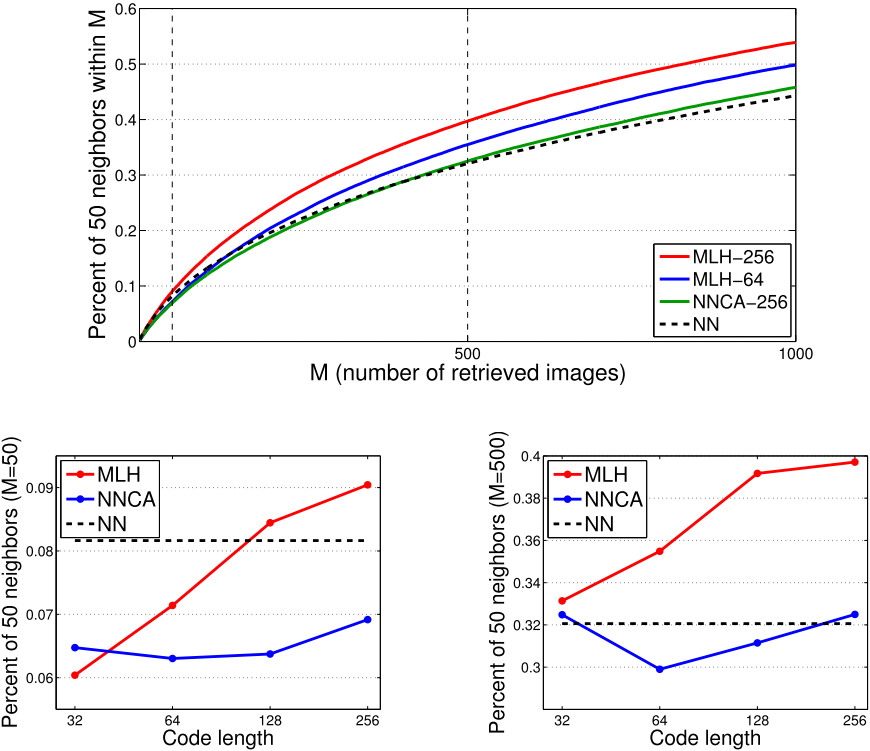
\includegraphics[width=\textwidth]{img/semantic_search_mlh_nnca.png}
	\caption{(top) Percentage of 50 ground-truth neighbors as a function of number of images retrieved ($0 \leq M \leq 1000$) for MLH with 64, 256 bits, and for NNCA with 256 bits. (bottom) Percentage of 50 neighbors retrieved as a function of code length for $M=50$ and $M=500$. \cite{norouzi2011minimal}}
	\label{fig:semantic_search_mlh_nnca}	
\end{figure*}

A second experiment, conducted by the authors of Triplet Loss Ranking (TRL) \cite{norouzi2012hamming}, compares it with MLH. Two data sets are used, MNIST and CIFAR-10. Similarity labels are derived from class labels: items from the same class are similar. In this review we only present the precision@k (fraction of same-class items from a kNN retrieval) on the MNIST data set for different hash functions, different optimization criteria and for different values of k. The results are plotted in figure \ref{fig:trl_vs_mlh}. The hash function is either a linear transformation or a two-layer neural network. The optimization method is either MLH or TRL. K varies from 1 to 10,000. A Euclidean nearest neighbor search is also included as baseline because it provides an upper bound on the performance of methods that preserve Euclidean distances (e.g. LSH). The conclusion is that TRL yields slightly better performances than MLH.

A third experiment, conducted by the authors of Minimal Loss Hashing (MLH) \cite{norouzi2011minimal}, compares it with NNCA, which is based on Semantic Hashing. The experiment makes use of the 22K LabelMe data set with a semantic pairwise affinity matrix provided by humans. As a consequence, the similarity is based on semantic content rather than on Euclidean distance. At the time this experiment was conducted, NNCA was considered as the superior method for this task. MLH and NNCA are trained, using varying code lengths, on 512D Gist features using the semantic labels. A nearest neighbor baseline using cosine similarity is added because it is a bound for LSH as it mimics Euclidean distance, which is worse than cosine similarity in Gist space. As shown in figure \ref{fig:semantic_search_mlh_nnca}, MLH and NNCA exhibit similar performance for 32-bit codes, but for longer codes MLH is superior.

According to these experiments, we have a rough idea on what are the relative performances of the previously described methods. MLH is clearly superior to LSH, Semantic Hashing appears to be less efficient than MLH. It is hard to compare Semantic Hashing with LSH because no experiment compares them directly. TRL is slightly better than MLH. The conclusion is however not perfectly reliable because the methods are not all compared at the same time. Moreover, it is based on experiments conducted by the authors of the methods.

MLH and TRL are the two best methods reviewed in this paper. Even if TRL is a generalization of MLH and appears to be slightly better, the two approaches have different use cases. On the one hand, MLH can preserve a metric structure with a pairwise similarity and $\rho$ allows one to search by range for similar images. On the other hand, TRL is well suited to the preservation of semantic similarity and since ranking is kept, one can perform a kNN to search for similar images.
\chapter{Search in Hamming Space}

\label{chapter:SearchHammingSpace}

% ----------------

\section{Exhaustive Sequential Search}
Because binary codes are storage efficient and comparisons are fast, a basic approach is to perform an exhaustive search by computing the distances to all codes in the database. This can be executed on processors and graphics processing units, and distributed on multiple computers.

Processors are well suited when all binary codes in the database fit in the cache. Indeed, the popcount instruction is so fast that the search is essentially limited by the throughput of the RAM. Moreover, if the search is executed on multiples cores cache miss problems can arise. Thus, memory bandwidth and cache are both performance factors. Therefore, processors are efficient for exhaustive sequential search up to about 5 million binary codes.

Graphics processing units (GPU) have higher computational power and memory bandwidth than processors. Moreover, the popcount instruction is also available. A certain number of binary codes is necessary to reach the best performance. Therefore, GPU are efficient for exhaustive sequential search starting from about 5 million binary codes.

\section{Hash Table}
The hash table lookup consists in creating a hash table on the binary codes. To perform a nearest neighbor search, we can retrieve the content of the hash buckets in the vicinity of a query code. The complexity, in this case, only depends on the length of binary codes and the search radius. For binary codes of $q$ bits, the number of distinct hash buckets to examine is \cite{norouzi2016}

\[V(q,r)=\sum\limits_{z=0}^r \binom{q}{z}\]

This approach is suited only for small distances because the number of hash buckets within a Hamming ball around a query grows almost exponentially with the search radius. For example, with 32 bits codes and a radius of 8 bits, about 15 million hash buckets are to explore, which is absurd if there are less than 15 million binary codes in the database, because an exhaustive sequential search would be faster. When binary codes are longer than 32 bits, which is often the case, the hash table approach is no more efficient.

A recent approach based on the idea of hash table lookup is Multi-Index Hashing (MIH) \cite{norouzi2012fast}, \cite{norouzi2016}, \cite{gog2016fast}. It consists in building multiple hash tables on binary code sub-strings and yield to sub-linear run-time behavior for uniformly distributed codes.

\section{Comparison}
In this section, we compare the performances of 3 methods: exhaustive sequential search with CPU and GPU, and Multi-Index Hashing. We implemented exhaustive sequential search on CPU with OpenMP \footnote{http://www.openmp.org} and on GPU with Thrust \footnote{https://developer.nvidia.com/thrust}. We use the implementation of Multi-Index Hashing from \cite{norouzi2012fast} \footnote{https://github.com/norouzi/mih}.

We compared the methods using the following protocol. A list of 64 bits binary codes is randomly generated with a uniform distribution. For each method, 10,000 fixed-radius nearest neighbor searches (with a radius fixed to 8) are performed with the first codes in the previously generated list. We measure the time to perform all queries along with the time to load data. We also check that all 3 methods are returning the same results.

Our benchmark is available on GitHub \footnote{https://github.com/mgaillard/HashSearch}. To get an idea of the actual performances we recommend running it directly on the concerned hardware. On commodity hardware, a Intel i5 Ivy Bridge and a GTX 750 Ti, for a large number of hashes (at least 50M) the MIH solution is the most efficient, followed by the GPU and finally the CPU (up to about 5M hashes). Depending on the hardware these results can vary. We compared the three methods on a server equipped with two Intel Xeon E5-2630 v3 and a Tesla K80 (we used only 1 of the 2 GPU), sequential search on the CPUs seems to be always better than GPU. MIH was better than sequential search on the CPU starting from about 100M hashes.

Sometimes, raw performance is not as important as power efficiency. In this case, one might want to compare the price-performance ratio. MIH only runs on one CPU core and is therefore the most efficient if the database contains enough hashes. Sequential search on CPU and GPU use all available cores and consume a lot of power, this is why they are less energy efficient.

\part{Contribution}
\chapter{Benchmarking}

\label{chapter:Benchmarking}

% ----------------

In a previous work \cite{gaillardlarge}, we designed a new framework to benchmark reverse image search engines. Our approach is based on the evaluation measures of information retrieval systems described in \cite{manning2008introduction}. We model the reverse image search engine as an information retrieval system that returns an unranked set of documents for a query. If many documents are retrieved, the user is in charge of choosing the one that best suit his needs.

\section{Metrics}

\subsection{Effectiveness}
To process a query, the reverse image search engine order the indexed images by relevance. Results are retrieved using a fixed-radius nearest neighbor search. Thus, each image, whether relevant for the query or not, can be retrieved or not. This notion can be made clear by examining the following contingency table \ref{table:contingency_table}.

\begin{table}[h]
\centering
\caption{Contindency table for information retrieval from \cite{manning2008introduction}}
\label{table:contingency_table}
\begin{tabular}{|c|c|c|}
\hline
              & Relevant            & Non-relevant        \\
\hline
Retrieved     & True positive (tp)  & False positive (fp) \\
\hline
Not retrieved & False negative (fn) & True negative (tn)  \\
\hline
\end{tabular}
\end{table}

The effectiveness of the system is measured with the following metrics: Precision (P) is the fraction of retrieved documents that are relevant,

\[precision=\mathbb{P}(\text{relevant}|\text{retrieved})=\frac{\text{\#(relevant items retrieved)}}{\text{\#(retrieved items)}}=\frac{tp}{tp+fp}\]

Recall (R) is the fraction of relevant documents that are retrieved.

\[recall=\mathbb{P}(\text{retrieved}|\text{relevant})=\frac{\text{\#(relevant items retrieved)}}{\text{\#(relevant items)}}=\frac{tp}{tp+fn}\]

A single measure that trades off precision versus recall is the F-measure, which is the weighted harmonic mean of precision and recall: 

\begin{align*}
F=\frac{(\beta^2+1)PR}{\beta^2P+R} && F_{\beta=1}=\frac{2PR}{P+R}
\end{align*}

It is possible to change the weights in the harmonic mean of the F measure in order to tune it. This is done by changing the $\beta$ parameter. Values of $\beta < 1$ emphasize precision, while values of $\beta > 1$ emphasize recall. This is important in order to benchmark the system in accordance with its application.

\subsection{Performance}
It is important to measure the time the system need for indexing and searching. Indeed, the system should be able to index millions of images and search across them as fast as possible. The complexity of both the indexing and searching phases depends on the number of images and is not necessarily linear. Therefore, we propose to measure the indexing and searching time for a certain number of images.

\section{Protocol}
\label{chapter:Benchmarking:section:Protocol}
In order to compare the effectiveness and the speed of different image search methods, we created a comparison protocol. We choose 25,000 images from the MIRFLICKR dataset\footnote{http://press.liacs.nl/mirflickr}.

To be able to calculate automatically the precision and recall of the results, we applied 6 small modifications on each image, that gave us a dataset with 175 000 images. We measured the index and search speed as well as the results precision and recall.

The modifications (illustrated on Figure \ref{fig:protocol_modifications}) applied on the images are: 

\begin{enumerate}
\item Gaussian blur ($r=4$, $\Sigma=2$)
\item Black and white transformation
\item Resize to half height and width
\item JPEG compression with $quality=10$
\item Clockwise rotation by 5 degrees
\item Crop by 10\% at the right side of the image. 
\end{enumerate}

\begin{figure*}
	\centering
	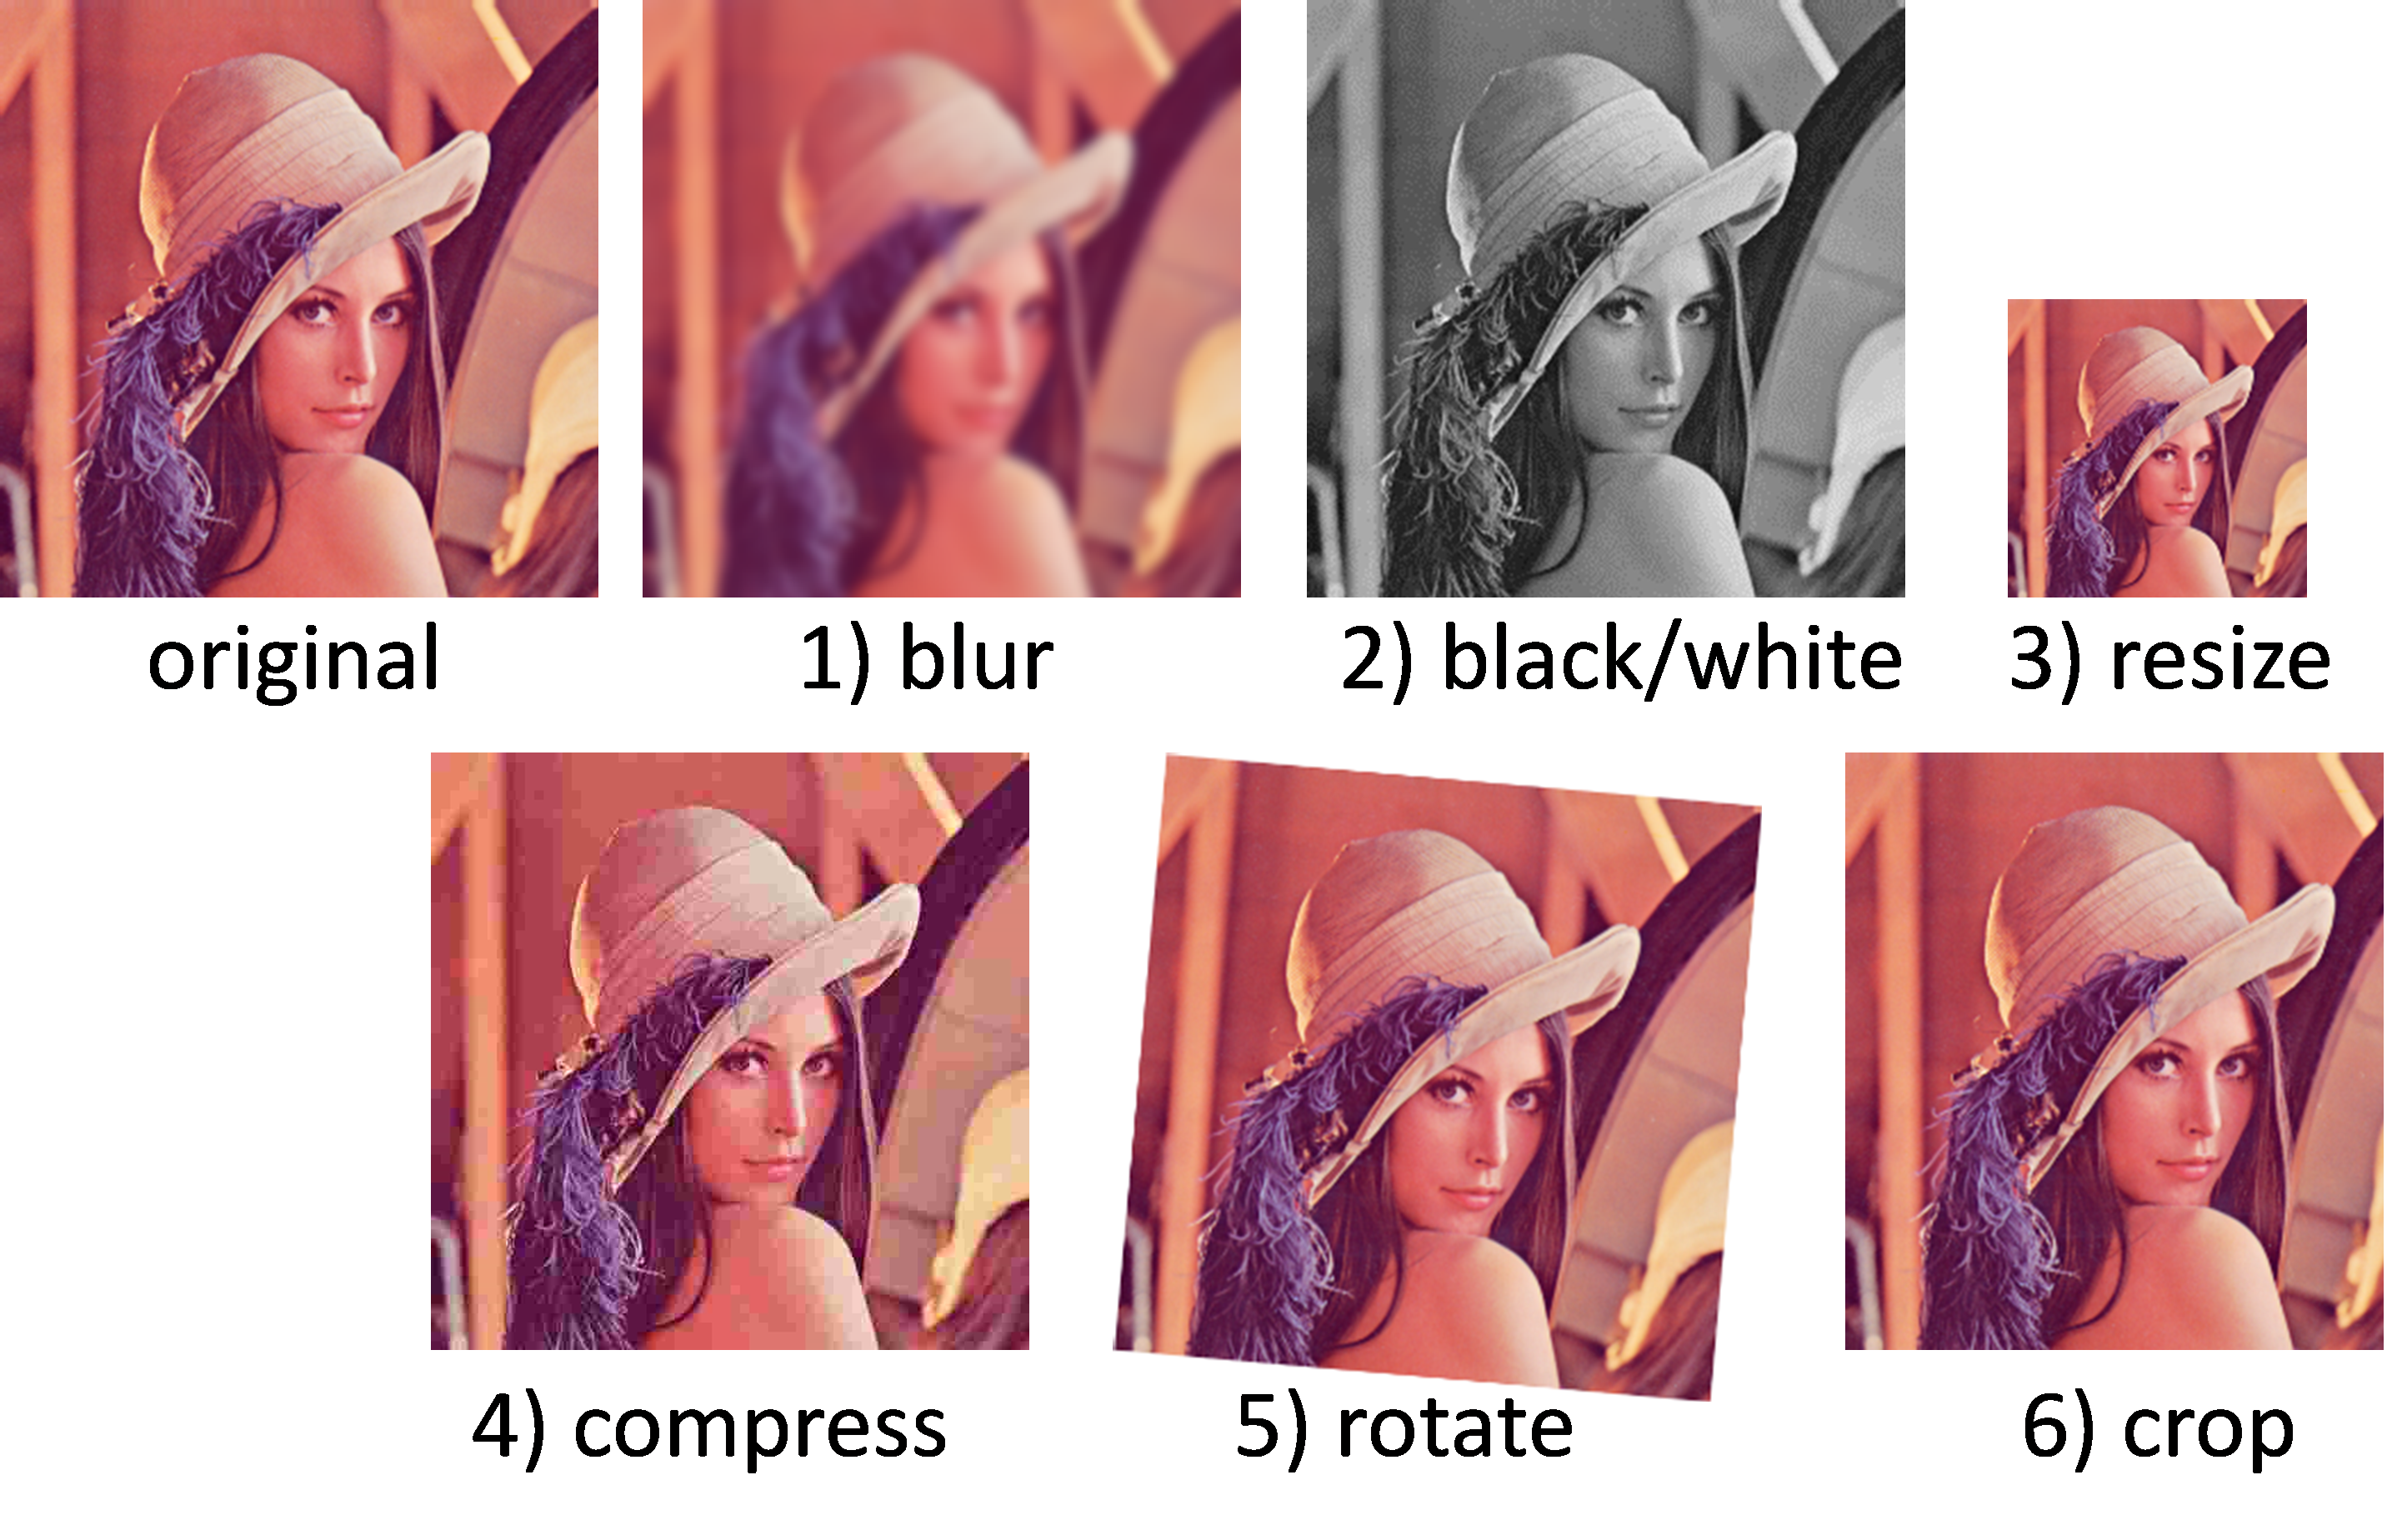
\includegraphics[width=\textwidth]{img/modifications.png}
	\caption{Illustration of the image modifications.}
	\label{fig:protocol_modifications}
\end{figure*}

These modifications represent the basic cases of small changes images usually undergo over the web. The benchmark is programmed so that it is easy to change the set of modifications.

Our benchmark protocol for a generic reverse image search engine is detailed in this section. 

\begin{enumerate}
	\item Select $N+M$ images that are representative to an application with no duplicated images. In our case $N=24,000$ and $M=1,000$ (the first 1,000 images from the dataset in alphabetical order)
	\item Split them into 2 sets of $N$ base images and $M$ non-indexed images.
	\item Select $K$ modifications and from the $N$ base images, generate $K$ new image sets containing $K \times N$ modified images. In our case $K=6$, and the modifications are those enumerated above.
	\item Index the $N$ base images and the $K \times N$ modified images according to the image representation method.
	\item Make search queries with:
		\begin{enumerate}
			\item The $M$ images from the non-indexed image set,
			\item The $N$ images from the base image set.
			\item The $K \times N$ images from the modified sets.
		\end{enumerate}
	\item Analyse the search results and compute the mean precision, the mean recall and the mean F-measure of all queries.
	\begin{enumerate}
		\item For the $M$ images of the non-indexed set, there should be no relevant result image. Thus, the result should be empty.
		\item When querying with one of the other $(K+1)\times N$ already indexed images, the relevant results are the $K+1$ images that are the modified version of the query image. Thus, the result of each query should contain K+1 images that come from the same base image as the query image.
	\end{enumerate}
\end{enumerate}

Because our system use a fixed-radius nearest neighbor search, we model it as an information retrieval system that returns an unranked set of documents. To determine the best radius, we repeat this protocol for several different radii.

It is possible to use the protocol in two different ways. Firstly, by applying all modifications to have an overview of the performances of a method. Thus, it is possible to compare two methods according to a complete workload. Secondly, by applying a single modification, for example to identify the strength and weakness of a method according to some modifications.

We implemented the protocol \footnote{See our implementation on: https://github.com/mgaillard/pHashRis} as Linux shell commands and C++, using online available libraries.

\section{Results}
\label{chapter:Benchmarking:section:Results}
We evaluate the methods described in chapter \ref{chapter:PerceptualHashing}: DCT, MH and RV based perceptual hash functions from \cite{zauner2010implementation}. 

\subsection{Retrieval performance against single modification}
We index the $N$ base images and then make $K$ search queries each with one of the $N$ modified images. We compute the F-measure for various radius and take the maximum.

\begin{figure*}
	\centering
	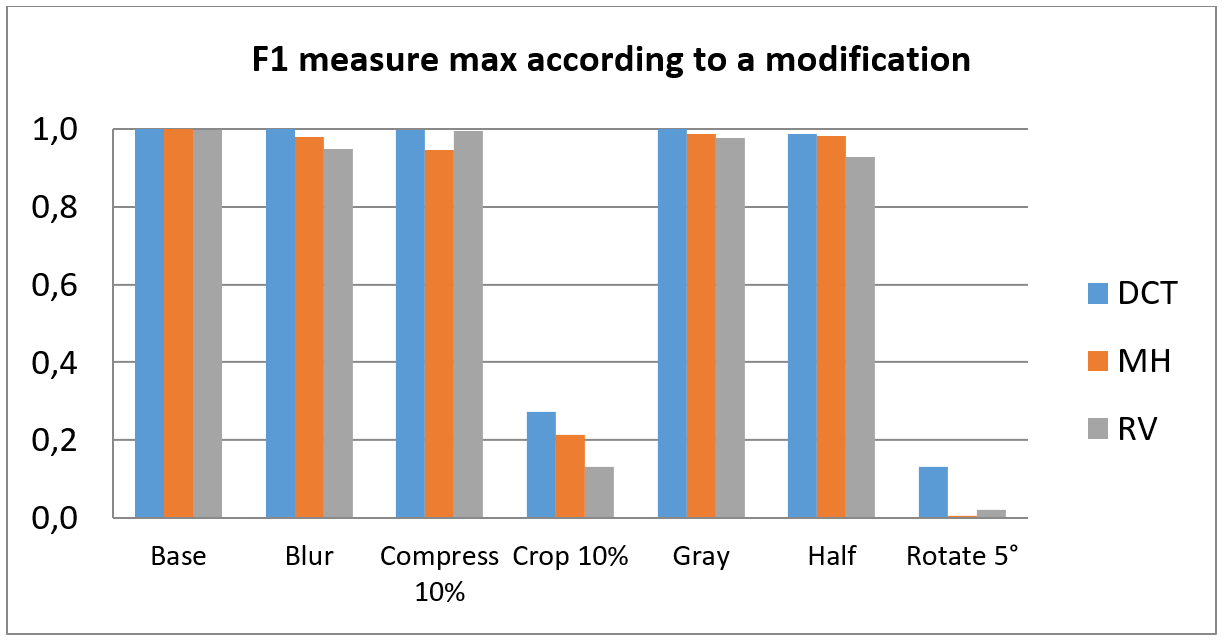
\includegraphics[width=\textwidth]{img/benchmark_single.png}
	\caption{Maximum F1-measure of DCT, MH and RV perceptual hash functions against single modifications.}
	\label{fig:benchmark_single}
\end{figure*}

The functions are robust against Gaussian blur ($r=4$, $\Sigma=2$), JPEG compression (quality 10\%), grayscale filter, and scale to half the size. However the functions are not robust against crop (10\% on the right) and rotate (5 degrees clockwise) modifications as illustrated on Figure \ref{fig:benchmark_single}.

We also tested, the evolution of our accuracy measures with different degrees of the modifications. We noticed that the different hash methods were quite sensible to rotations (above 2 degrees) or to cropping (above 5\%), but resisted very well to compression, blur or resize.

\subsection{Retrieval performance against all modifications}
To evaluate the speed and retrieval performance of a reverse image search engine, we run the protocol described in the previous section. The results are in figures \ref{fig:benchmark_dct}, \ref{fig:benchmark_mh}, \ref{fig:benchmark_rv}. We can see that all functions have equivalent retrieval performances with a maximum F-measure of about 60%.

The results (table \ref{table:benchmark_times}) showed that the DCT based hash function is clearly faster than the Marr-Hildert (MH) Operator and Radial Variance (RV) based hash functions. It is also more accurate against the 6 chosen modifications. We evaluate the retrieval performance, calculating the mean precision, recall and F-measure of the returned results. The calculation is repeated for different radius values. The radius here is a normalized distance value, below which two images are considered as similar.

The performance is evaluated through the index and search speed. Table \ref{table:benchmark_times} presents the measurements done for 125,000 images on an OVH dedicated virtual machine equipped with an Intel Xeon Haswell 8 cores at 3.1 GHz and 30 GB of RAM.

\begin{figure*}
	\centering
	\begin{tabular}{|c|c|c|}
		\hline
				& Index 125k images   & 125k queries on 125k images \\
		\hline
		DCT & 3 min 55 sec        & 3 min 59 sec                \\
		\hline
		MH  & 31 min 13 sec       & 32 min 20 sec               \\
		\hline
		RV  & 1 min 48 sec        & 3h 47 min 31 sec            \\
		\hline
	\end{tabular}
	\caption{indexing and search time measures for the DCT, MH and RV based perceptual hash functions}
	\label{table:benchmark_times}
	
	\includegraphics[width=\textwidth]{img/benchmark_dct.png}
	\caption{Precision/Recall/F-measure curves of the DCT based perceptual hash function search results according to different radius values}
	\label{fig:benchmark_dct}
\end{figure*}

\begin{figure*}
	\centering
	\includegraphics[width=\textwidth]{img/benchmark_mh.png}
	\caption{Precision/Recall/F-measure curves of the Marr-Hilderth based perceptual hash function search results according to different radius values}
	\label{fig:benchmark_mh}
	
	\includegraphics[width=\textwidth]{img/benchmark_rv.png}
	\caption{Precision/Recall/F-measure curves of the Radial Variance based perceptual hash function search results according to different radius values}
	\label{fig:benchmark_rv}
\end{figure*}
\chapter{CNN Features Robustness}

\label{chapter:CNNFeaturesRobustness}

% ----------------

\section{Introduction}
In a previous chapter \ref{chapter:ConvolutionalNeuralNetworks}, we advocate the use of convolutional neural networks to extract features from images. In this chapter, we evaluate the robustness of CNN features against modifications. In a first time, instead of trying to learn an image representation from scratch, we assess the robustness of existing networks trained on an unrelated classification task. The aim being to find an already good representation, according to a specific distance, whose dimensionality would be reduced later. This step is important because we make the hypothesis that an already robust image representation will still stay more robust after a dimensionality reduction than a less robust image representation. Despite breaking our main problem into two sub problems (features extraction and dimensionality reduction) is certainly not optimal, depending on the dimensionality reduction method, it is possible to fine tune the image representation. It is for example possible with methods based on neural networks such as: Minimal Loss Hashing and Triplet Ranking Loss. By optimizing at the same time the image representation and the dimensionality reduction, the retrieval performance should probably be better.

\section{Protocol}
The protocol is inspired from our previous benchmark for Reverse Image Search described in chapter \ref{chapter:Benchmarking}. It is based on a set of images that are modified according to some transformations. We then consider a base image and its modified versions as similar amongst themselves, and all other pairs of images as dissimilar. All images are queried and the average precision, recall and Fmeasure are computed over all queries.

\subsection{Preparation}
Following are the steps to prepare images for the benchmark.

\begin{enumerate}
	\item Select $N$ images that are representative to an application with no duplicated images. In our case, $N$ is equal to either 200, 2500 or 25,000.
	\item Select $K$ modifications and from the $N$ base images, generate $K$ new image sets containing $K \times N$ modified images. In our case $K=6$, and the modifications are those enumerated in section \ref{chapter:Benchmarking:section:Protocol}: blur, grayscale, resize, JPEG compression, rotation and cropping.
	\item With a convolutional neural network, extract the features from all images. More details about this step are given in section \ref{chapter:CNNFeaturesRobustness:section:Models}.
\end{enumerate}

\subsection{Distribution of distances}
To get a rough idea of the robustness of CNN features against modifications, we analyze the distribution of distances between similar and dissimilar images. It is also useful to know the distribution of distances for the RIS benchmark. In fact, we can infer an approximate value for the best radius separating similar and dissimilar images.

\begin{enumerate}
	\item For each modification, compute the distance between each base image and its modified version. Take this distance in account in the computation of the minimum, first quartile, median, last quartile and maximum distance between the base and the modified image set. Draw a box plot with these data.
	\item For each pair of different images in the base image set, compute the distance between them.  Take this distance in account in the computation of the minimum, first quartile, median, last quartile and maximum distance between dissimilar images. Draw a box plot with these data.
\end{enumerate}

The resulting box plots can be seen in the Result section \ref{chapter:CNNFeaturesRobustness:section:Results} of this chapter. Ideally, the distribution of distances should not overlap. In other words, the distances between similar images must be strictly smaller than the distances between dissimilar images.

\subsection{RIS benchmark}
To get a precise idea of the retrieval performance using CNN features, we implement the same benchmark as in chapter \ref{chapter:Benchmarking}. We compute all distances between all pairs of images and apply a threshold below which images are considered as similar. Then we compute the mean precision, the mean recall and the mean F-measure. The protocol is repeated for various threshold, the threshold that maximizes the F-measure can be considered as the best radius for the reverse image search system.

\begin{enumerate}
	\item Make search queries with the $(K+1) \times N$ images from the base and modified sets.
	\item Analyse the search results and compute the mean precision, the mean recall and the mean F-measure of all queries.
	\begin{enumerate}
		\item The relevant results are the $K+1$ images that are the modified version of the query image. Thus, the result of each query should contain K+1 images that come from the same base image as the query image.
	\end{enumerate}
\end{enumerate}

The resulting plots can be seen in the Result section \ref{chapter:CNNFeaturesRobustness:section:Results} of this chapter. More detailed results for \textit{VGG16\_block5\_pool\_max} with Cosine distance are available in appendix \ref{chapter:ResultsVGG16Block5PoolMax}. Ideally, the maximum F-measure should be near to 1.

\section{Models}
\label{chapter:CNNFeaturesRobustness:section:Models}
In this section, we describe all models compared in the benchmark. To extract the features, we use a pretrained neural network to predict the label of an image. The feature vector consists of the activations of the units of one specific layer. If the layer is a convolutional or pooling layer, the results are 2D features maps. In this case, the activations are flattened using a global average or maximum pooling. We compare the models described in section \ref{chapter:ConvolutionalNeuralNetworks:section:Models}: \textit{VGG16}, \textit{VGG19}, \textit{ResNet50}, \textit{InceptionV3}. We also evaluate \textit{Xception}, which is also a model available in Keras. If needed the feature vectors can be normalized to unit length in Euclidean distance. To compare the feature vectors, two distances are used: Euclidean and Cosine. 

In the following sections, we describe, for all models, all layers that we compared. The name of layers are the same as in the Keras library. For the models, the naming convention we use in the program is: [network]\_[layer]. If the feature vector is normalized with L2 we add \textit{\_norm\_l2} at the end. For example, \textit{ResNet50\_flatten\_1\_norm\_l2} is extracted from the \textit{flatten\_1} layer of the \textit{ResNet50} network and is normalized as unit length in Euclidean distance.

\subsection{VGG}
In VGG16 and VGG19, available layers ordered by increasing depth are:
\begin{itemize}
	\item block\{\textit{i}\}\_pool\_avg for $i \in \{3, 4, 5\}$
	\item block\{\textit{i}\}\_pool\_max for $i \in \{3, 4, 5\}$
	\item flatten
	\item fc1
	\item fc2
	\item predictions
\end{itemize}

\subsection{ResNet50}
In ResNet50, available layers ordered by increasing depth are:
\begin{itemize}
	\item activation\_\{\textit{i}\}\_avg for $i \in \{4, 7, 10, 13, 16, 19, 22, 28, 31, 34, 37, 40, 43, 46\}$
	\item activation\_\{\textit{i}\}\_max for $i \in \{4, 7, 10, 13, 16, 19, 22, 28, 31, 34, 37, 40, 43, 46\}$
	\item avg\_pool\_avg
	\item avg\_pool\_max
	\item flatten\_1
	\item predictions
\end{itemize}

\subsection{InceptionV3}
In InceptionV3, available layers ordered by increasing depth are:
\begin{itemize}
	\item mixed\{\textit{i}\}\_avg for $i \in \{0, 1, 2, 3, 4, 5, 6, 7, 8, 9, 10\}$
	\item mixed\{\textit{i}\}\_max for $i \in \{0, 1, 2, 3, 4, 5, 6, 7, 8, 9, 10\}$
	\item predictions
\end{itemize}

\subsection{Xception}
In Xception, available layers ordered by increasing depth are:
\begin{itemize}
	\item add\_\{\textit{i}\}\_avg for $i \in \{1, 2, 3, 4, 5, 6, 7, 8, 9, 10, 11, 12\}$
	\item add\_\{\textit{i}\}\_max for $i \in \{1, 2, 3, 4, 5, 6, 7, 8, 9, 10, 11, 12\}$
	\item block14\_sepconv1\_act\_avg
	\item block14\_sepconv1\_act\_max
	\item block14\_sepconv2\_act\_avg
	\item block14\_sepconv2\_act\_max
	\item predictions
\end{itemize}

\section{Implementation}
Our implementation is on GitHub \footnote{https://github.com/mgaillard/CNNFeaturesRobustness}. It consists of three main programs and a bash script to orchestrate their executions.

The first program is a Python script that extracts features from images using the neural network library Keras \cite{chollet2015keras}. The feature vectors can be saved in HDF5 files, which are then read during the execution of the second and third programs.

The second program is the implementation of the distance benchmark. It computes statistics on the distribution of distances between similar and dissimilar images. Those are first written in a file and then used to generate a plot with gnuplot.

The third program is the RIS benchmark. It is written in C++ with OpenMP, to fasten the computation of distances in high dimensional spaces thanks to multi-threading and SIMD. This benchmark computes the mean precision, recall and F-measure of a RIS system based on the previously extracted features. The results are first written in a file and then used to generate a plot with gnuplot.

The workflow of the bash script is:
\begin{enumerate}
	\item Images are modified according to the $K$ modifications with ImageMagick \footnote{www.imagemagick.org}.
	\item Features are extracted from the $(K+1) \times N$ images according to all possible models.
	\item The distance benchmark is executed for all features according to Euclidean and Cosine distance.
	\item The RIS benchmark is executed for all features according to Euclidean and Cosine distance.
\end{enumerate}

\section{Results}
\label{chapter:CNNFeaturesRobustness:section:Results}

Because the benchmark is compute intensive, to find the best model we proceed in three steps. Firstly, we compare all models with all distances but only with 200 images. We retain only the models whose F-measure is above 90\%. Secondly, we repeat this process with 2,500 images. The best models with 2500 images ordered by decreasing F-measure are:

\begin{itemize} 
	\item \textit{VGG16\_flatten} with Cosine distance; $Fmeasure = 0,952$
	\item \textit{VGG19\_flatten} with Cosine distance; $Fmeasure = 0,949$
	\item \textit{ResNet50\_activation\_46\_max} with Cosine distance; $Fmeasure = 0,948$
	\item \textit{ResNet50\_activation\_43\_max} with Cosine distance; $Fmeasure = 0,941$
	\item \textit{VGG16\_block5\_pool\_max} with Cosine distance; $Fmeasure = 0,931$
	\item \textit{VGG19\_block5\_pool\_max} with Cosine distance; $Fmeasure = 0,929$
	\item \textit{InceptionV3\_mixed9\_max} with Cosine distance; $Fmeasure = 0,918$
	\item \textit{InceptionV3\_mixed9\_avg} with Cosine distance; $Fmeasure = 0,911$
\end{itemize}

Finally, we compare these models with all the 25,000 images from the MIRFLICKR collection.

\subsection{Distribution of distances}
In figure \ref{fig:distributions_VGG16_block5_pool_max_cosine}, we present the distribution of distances obtained with \textit{VGG16\_block5\_pool\_max} with Cosine distance. Only one model is presented because this benchmark is not as precise as the RIS benchmark, and is mainly used to get an idea of the value of the best radius. Moreover, all models have similar distribution of distances.

\begin{figure*}
	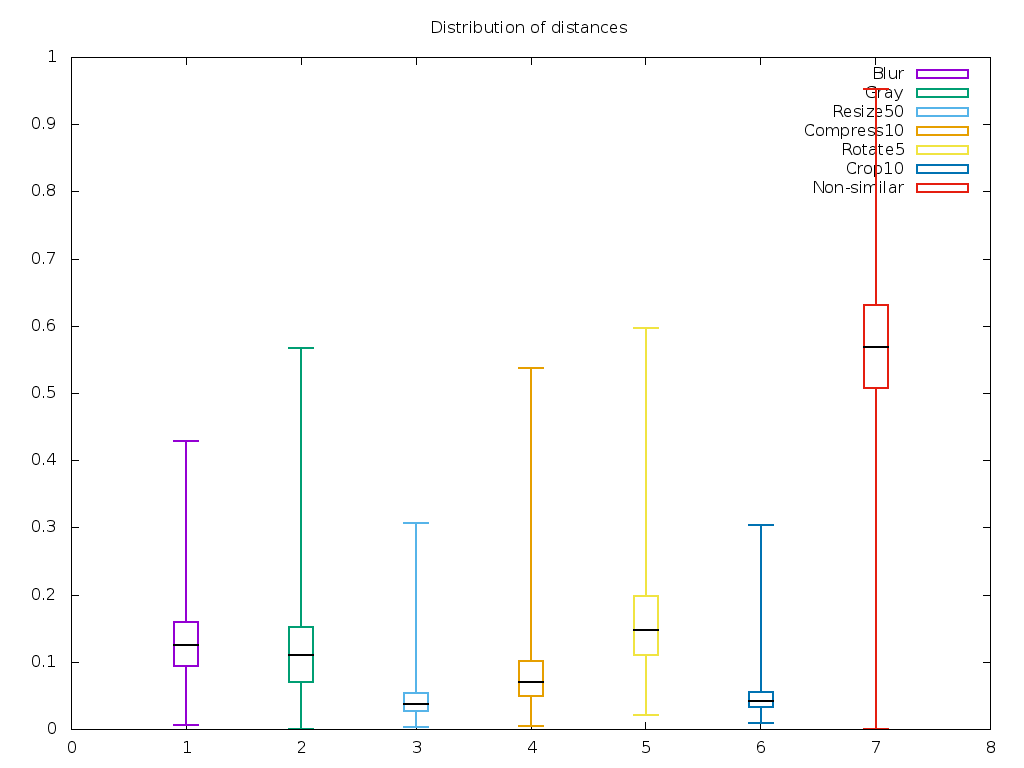
\includegraphics[width=\textwidth]{img/distributions_VGG16_block5_pool_max_cosine.png}
	\caption{Distribution of distances according to a modification obtained with \textit{VGG16\_block5\_pool\_max} with Cosine distance}
	\label{fig:distributions_VGG16_block5_pool_max_cosine}
\end{figure*}

We can see that distances between base and modified images are statistically smaller than the distances between dissimilar images. The interquartile ranges are especially not overlapping, which means that it is possible to differentiate the majority of similar and dissimilar images. The median distance between dissimilar images is about 0.6. If one uses this value as radius for the nearest neighbor search, approximately half of all images would be retrieved. Depending on the modification, the distribution of distances is not the same. Distances between base images and images that are resized to 50\% or cropped by 10\% on the right are smaller than for other modifications. Consequently, we can say that features extracted with \textit{VGG16\_block5\_pool\_max} are more robust to resize and cropping than JPEG compression, grayscale filter, Gaussian blur and rotation.

\subsection{RIS benchmark}

\subsubsection{Retrieval performance against all modifications}
The results of the benchmark with all modifications are shown in table \ref{table:benchmark_all}. Each line represents the maximum F-measure of each model along with the corresponding radius, precision and recall.

\begin{table*}
	\centering
	\caption{Benchmark with all modifications on 25,000 images: maximum Fmeasure}
	\label{table:benchmark_all}
	\begin{tabular}{|crcrrrr|}
	\hline
	Model                         & Dimensions & Distance & Radius & Precision & Recall & Fmeasure \\
	\hline
	VGG16\_flatten                &      25088 & cosine   &   0,51 &     0,954 &  0,943 &    0,936 \\
	VGG19\_flatten                &      25088 & cosine   &   0,50 &     0,955 &  0,934 &    0,931 \\
	ResNet50\_activation\_46\_max &       2048 & cosine   &   0,17 &     0,968 &  0,913 &    0,928 \\
	ResNet50\_activation\_43\_max &       2048 & cosine   &   0,14 &     0,952 &  0,919 &    0,921 \\
	VGG16\_block5\_pool\_max      &        512 & cosine   &   0,23 &     0,947 &  0,898 &    0,904 \\
	VGG19\_block5\_pool\_max      &        512 & cosine   &   0,23 &     0,948 &  0,892 &    0,902 \\
	InceptionV3\_mixed9\_max      &       2048 & cosine   &   0,20 &     0,926 &  0,892 &    0,881 \\
	InceptionV3\_mixed9\_avg      &       2048 & cosine   &   0,20 &     0,924 &  0,865 &    0,866 \\
	\hline
	\end{tabular}
\end{table*}

We can see that despite the fact that the F-measure decreases by about 3 points with 25,000 images compared to 2,500 images, the F-measures are still very good. For comparison, on the same benchmark, the DCT based perceptual hash function yields to a F-measure of about 0.6 (cf. section \ref{chapter:Benchmarking:section:Results}).

\subsubsection{Retrieval performance against single modification}
The results of the benchmark with single modifications are shown in table \ref{table:cnn_benchmark_single} and in figure \ref{fig:cnn_benchmark_single}. Each bar represents the maximum F-measure of each model against a single modification. The radius at which the F-measure is maximum can vary depending on the model and the modification. Thus, this figure gives an idea of the best retrieval accuracy against a single modification. This is why individually the F-measure is better than in the benchmark against all modifications. Because in this latter, the radius is the same for all modifications.

\begin{sidewaysfigure*}
	\centering
	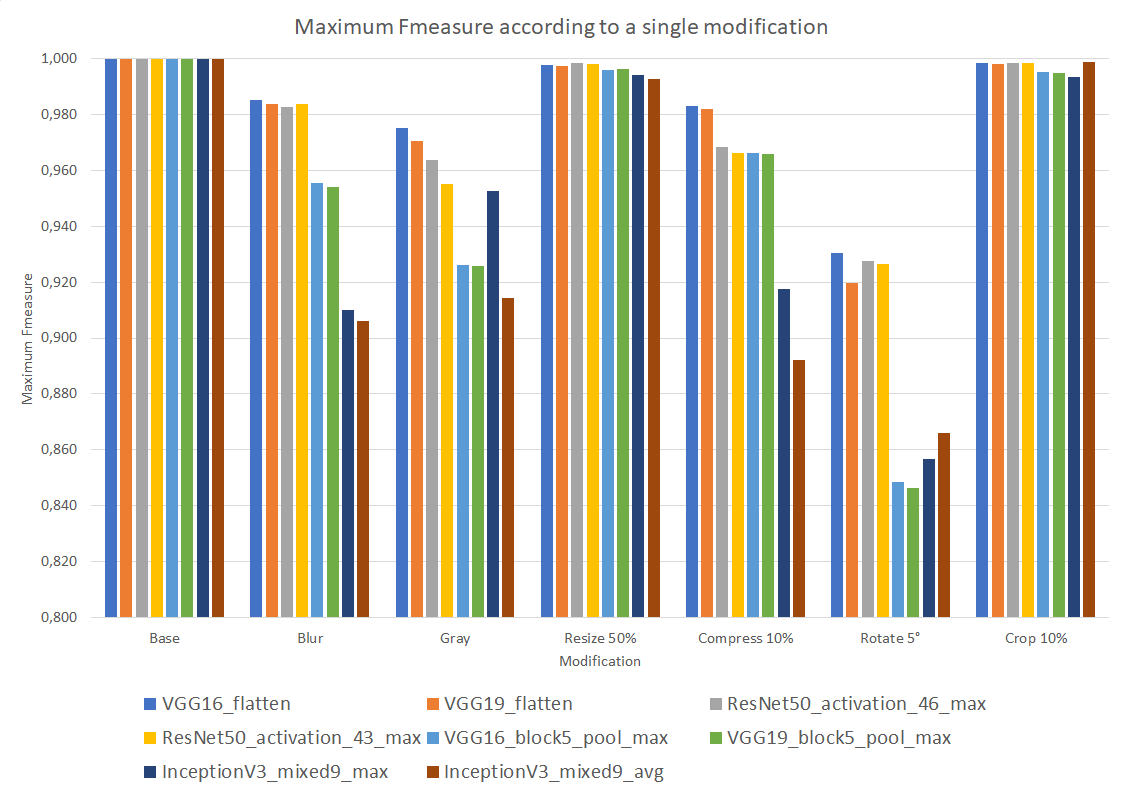
\includegraphics[totalheight=0.7\textheight]{img/cnn_benchmark_single.png}
	\caption{Maximum Fmeasure of CNN models against single modifications}
	\label{fig:cnn_benchmark_single}
\end{sidewaysfigure*}

\begin{table*}
	\begin{tabular}{|l|rrrrrrr|}
    \hline
                                  &  Base &  Blur &  Gray & Resize & Compr & Rotate &  Crop  \\
    \hline                                                                           
    VGG16\_flatten                & 1,000 & 0,985 & 0,975 &  0,998 & 0,983 &  0,930 & 0,998  \\
    VGG19\_flatten                & 1,000 & 0,984 & 0,971 &  0,998 & 0,982 &  0,920 & 0,998  \\
    ResNet50\_activation\_46\_max & 1,000 & 0,983 & 0,964 &  0,998 & 0,968 &  0,928 & 0,998  \\
    ResNet50\_activation\_43\_max & 1,000 & 0,984 & 0,955 &  0,998 & 0,966 &  0,927 & 0,999  \\
    VGG16\_block5\_pool\_max      & 1,000 & 0,955 & 0,926 &  0,996 & 0,966 &  0,848 & 0,995  \\
    VGG19\_block5\_pool\_max      & 1,000 & 0,954 & 0,926 &  0,996 & 0,966 &  0,846 & 0,995  \\
    InceptionV3\_mixed9\_max      & 1,000 & 0,910 & 0,953 &  0,994 & 0,917 &  0,857 & 0,994  \\
    InceptionV3\_mixed9\_avg      & 1,000 & 0,906 & 0,914 &  0,993 & 0,892 &  0,866 & 0,999  \\
    \hline
	\end{tabular}
	\caption{Maximum Fmeasure of CNN models against single modifications. Bar chart in figure \ref{fig:cnn_benchmark_single}.}
	\label{table:cnn_benchmark_single}
\end{table*}

We can see that all models work well and their F-measures are at least above 0.8. All models are very robust against resize to half-size and cropping 10\% on the right, with a F-measure greater than 0.99. The robustness against Gaussian blur, grayscale filter and JPEG compression is good, with a F-measure greater than 0.9. Rotation is the harder modification, with a F-measure of about 0.85 for \textit{VGG16\_block5\_pool\_max}, \textit{VGG19\_block5\_pool\_max}, \textit{InceptionV3\_mixed9\_max} and \textit{InceptionV3\_mixed9\_avg}, and about 0.92 for the others. Models based on \textit{ResNet50} yields to the best results for all modifications.

\subsection{Conclusion}
The objective of this chapter is to find an image representation that is robust against modifications. In chapter \ref{chapter:Benchmarking}, we compare different perceptual hash functions, which can be used as image representation, and show that they are not robust against cropping and rotation. In this chapter, we compare features extracted with off the shelf convolutional neural networks and find a set of models that have very good retrieval performances against modifications. Especially, these are quite robust against rotation and very robust against cropping. 

Robustness is certainly caused by preprocessing and data augmentation during training. Because the input of the convolutional neural network has always a constant size, images are first resized, thus features are robust against scaling. During training, it is common to generate more samples by transforming original images. For example, during the training of VGG \cite{simonyan2014verydeep}, to obtain the fixed size input images, training images are randomly cropped from rescaled training images. Therefore, the neural network is forced to learn a representation that is robust against cropping. More generally, by choosing the modifications made during the data augmentation step, one could give the neural network the ability to be robust against these modifications.

Two different distances are used to compare feature vectors: Euclidean and Cosine. However, it appears that cosine distance yields better results than Euclidean distance. We suppose that it is because, with convolutional neural networks, a neuron is activated with the presence of a feature. The level of presence of the feature is not as important as the fact that it is present.

Of course, CNN features are very robust against modifications but they are not suited for large scale applications. Indeed, the dimensionality of CNN feature vectors is very high. For more details, see the dimensions column of table \ref{table:benchmark_all}. As explained in chapter \ref{chapter:ReverseImageSearch}, it is currently impossible to index $p$-dimensional feature vectors when $p$ is greater than 20. For a large-scale application, one should reduce the dimension of the CNN feature vectors. In the next chapter, we present a method to map feature vectors into binary codes that preserve similarity.
\chapter{CNN Features Hashing}

\label{chapter:CNNFeaturesHashing}

% ----------------

% ---------------- Section: Introduction ----------------
\section{Introduction}
In a previous chapter \ref{chapter:HashingDimensionalityReduction}, we advocate the use of small binary codes and hashing for nearest neighbor search. In this chapter, we present a new approach for hashing into binary codes inspired from LSH with random projection and Minimal Loss Hashing, which are detailed in \ref{chapter:HashingDimensionalityReduction}.
	
Our approach is based on the same space partitioning as LSH with random projection and on the same cost function as Minimal Loss Hashing, it is therefore a supervised learning approach. The space is partitioned with a set of hyperplanes, each of them being responsible for the value of one bit in the binary code. If a point is on one side of a hyperplane, the associated bit takes a value of 1 and if the point is on the other side, the bit takes a value of 0. The difference between Minimal Loss Hashing and our approach is the optimization method. Minimal Loss Hashing builds a convex-concave upper bound on the loss function and a stochastic gradient-based method is used to minimize the bound function. On our side, we optimize the cost function in a continuous space. During the training, instead of binary codes, our algorithm generates $q$-dimensional vectors whose elements are in $[0, 1]$. Because codes are continuous, optimization is easier. Once training is done, $q$-dimensional vectors are binarized with a threshold to obtain binary codes.

% ---------------- Section: Formulation ----------------
\section{Formulation}
The task is to find a hash function that maps $p$-dimensional vectors, $x\in\mathbb{R}^{p}$, into $q$-bit binary codes, $h\in\mathbb{H}\equiv\{0, 1\}^{q}$, while preserving similarity:

\[b: \mathbb{R}^{p} \mapsto \{0, 1\}^{q}\]

The family of hash function that we consider is a thresholded linear transformation, parametrized by $W \in \mathbb{R}^{q \times p}$:

\[b_{W}(x) = thr(Wx)\]

where $thr(\cdot)$ is an element-wise Heaviside function. The space is partitioned with a set of hyperplanes, each of them being responsible for the value of one bit in the binary code. If a point is on one side of a hyperplane, the associated bit takes a value of 1 and if the point is on the other side, the bit takes a value of 0. For more details, see chapter \ref{chapter:HashingDimensionalityReduction}.

The objective is to optimize the values of elements in $W$ so that the notion of similarity is as far as possible preserved in Hamming space.

% ---------------- Section: Our approach ----------------
\section{Our approach}
The previously defined hash function is hard to optimize because its output is discontinuous due to the $thr(\cdot)$ function. To address this problem, we make binary codes continuous, $c \in [0, 1]^{q}$, during training by ignoring the $thr(\cdot)$ function and applying an element-wise sigmoid function. The sigmoid function is used to hold the results of the projections between 0 and 1.

\[c_{k;W}(x) = sigmoid_k(Wx) = \frac{1}{1 + e^{-kWx}} \text{ with } k \in \mathbb{R}_+\]

If the result of $c_{k;W}(x)$ is binarized with a threshold of 0.5, it is equivalent to $b_{W}(x)$. To extend the Hamming distance on binary codes to continuous codes, we use an element-wise L1 norm.

\[d_{continuous}(c, c') = \norm{c - c'}_{C} = \sum\limits_{i=1}^q \left|c_i-c'_i\right| \text{ with } c, c' \in [0, 1]^{q}\]

We can see that if the two continuous codes are composed only of binary values, $d_{continuous}$ is equivalent to Hamming distance on binary codes. It is also important to note that if two elements have values of 0.5, the distance between them will be exactly zero. This can be annoying because the optimization can fall in a situation where element values are 0.5 (See figure \ref{fig:continuous_hamming_distance}). To prevent the optimization from doing that, we can add a regularization term to the distance that penalizes elements that are not near to 0 or 1.

\begin{figure*}
	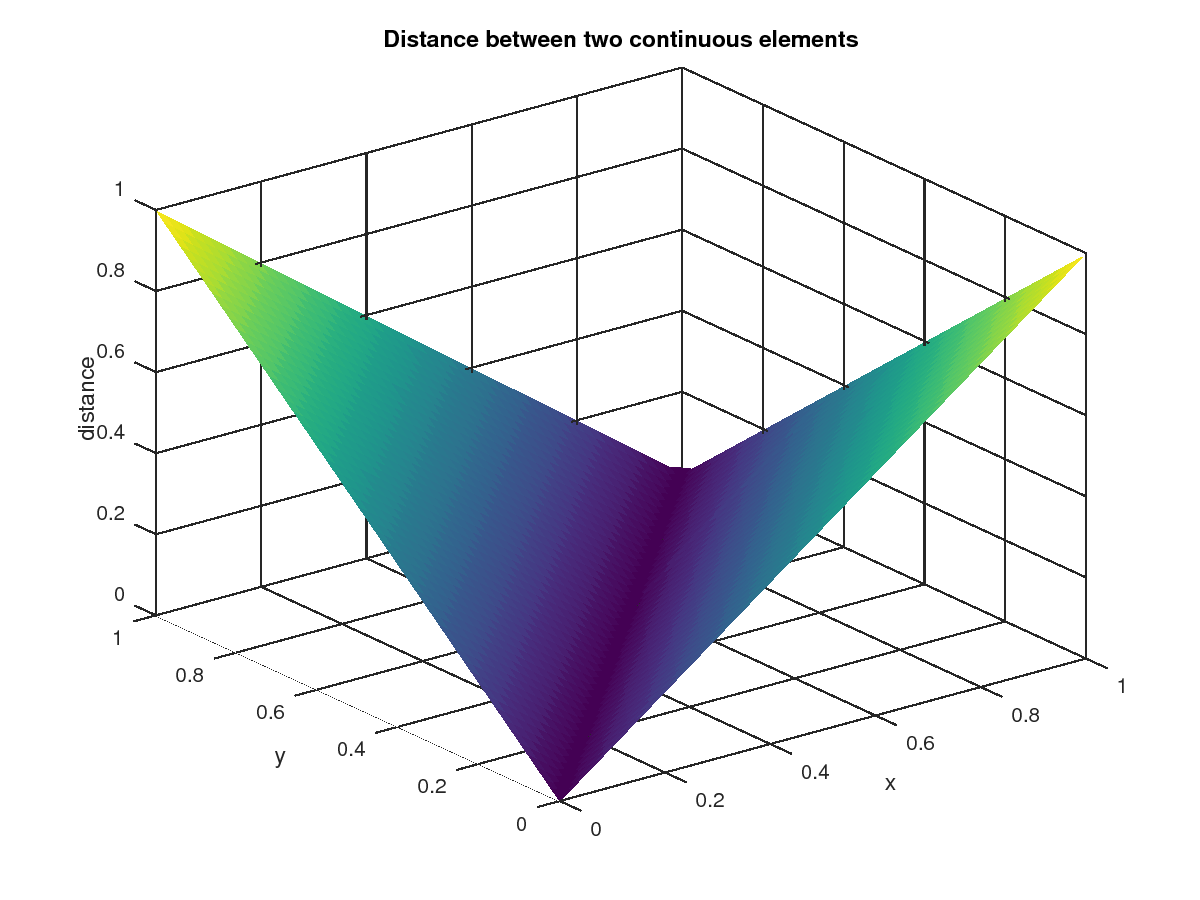
\includegraphics[width=\textwidth]{img/continuous_hamming_distance.png}
	\caption{Surface of the distance function between two continuous elements.}
	\label{fig:continuous_hamming_distance}
\end{figure*}

\subsubsection{Dataset}
The learning is based on a training data set of labeled pairs $(x_i, x'_i, s_i)$ where $x_i$ and $x'_i$ are $p$-dimensional centered training points and $s_i$ is a similarity label, whose value is 1 if $x_i$ and $x'_i$ are similar and 0 if dissimilar. To preserve a specific metric, one can compute the similarity label by thresholding the pairwise distance. Alternatively, to preserve the semantic similarity, one can assign a similarity label based on the class label. It is important to note that, if we want an exhaustive set of pairs, the number of pairs grows quadratically with the number of input vectors. With $n$ images, there are $\frac{n(n-1)}{2}$ pairs (2-combination) of input vectors.

\[D \equiv \{x_i, x'_i, s_i\}_{i=1}^N \text{ with } x_i, x'_i \in \mathbb{R}^{p} ; s_i \in \{0, 1\} \]

\subsubsection{Preprocessing}
In our implementation, it is possible to preprocess input vectors before training. Available preprocessing steps are: PCA, mean-centering and normalization to unit length, always executed in this order. Usually, only mean-centering and normalization are activated. PCA is simply implemented for experiments, to evaluate the impact of decorrelation and dimensionality reduction before hashing.

\subsubsection{Loss function}
To optimize the values of the parameters of the hash function, we define a cost function that is minimal when similarity is preserved. The cost function is inspired from Minimal Loss Hashing \cite{norouzi2011minimal}. For each pair of input vectors in the training data set, a loss function $l_{pair}: [0, 1]^{q}\times[0, 1]^{q}\times\{0, 1\}\mapsto\mathbb{R}^{+}$ assesses the quality of the mapping by assigning a cost to a pair of continuous codes and a similarity label. The cost function penalizes similar (resp. dissimilar) samples that are mapped onto continuous codes that are dissimilar (resp. similar). By minimizing the loss over all training examples, we can learn the best parameters of the hash function.

We introduce the hyperparameter $\rho$, which is a threshold of distance in Hamming space, that defines the boundary between similar and dissimilar codes. If the distance between two codes is less than (resp. more than) $\rho$ we can consider them as similar (resp. dissimilar). Although it is a slow process, a good value for this hyper parameter can be found with a validation set.

In addition, the $\lambda$ parameter adjusts the penalty incurred for dissimilar pairs when they are too close in comparison to the penalty incurred for similar pairs when they are too far from each other. In the case that there are significantly less pairs of similar images than pairs of dissimilar images, the optimization method can find a solution where all codes are different because it satisfies the majority of constraints. To mitigate this effect, $\lambda$ is equal to the number of similar pairs divided by the number of dissimilar pairs.

\[\lambda = \frac{\sum\limits_{i=1}^N s_i}{N - \sum\limits_{i=1}^N s_i}\]

Let $\norm{c - c'}_{C}$ be the continuous Hamming distance between continuous codes $c$ and $c'$. The pairwise loss based on the hinge function is defined as:

\[
	l_{pair}(c, c', s)=
	\begin{cases}
	\max(\norm{c - c'}_{C} - \rho, 0) & \text{for } s=1 \\
	\lambda\max(\rho - \norm{c - c'}_{C} + 1, 0) & \text{for } s=0
	\end{cases}
\]

\[
\begin{split}
L_{continuous}(W) & = \sum\limits_{i=1}^N l_{pair}(c_{k;W}(x_i), c_{k;W}(x'_i), s_i) \\
                  & = \sum\limits_{i=1}^N s_i\max(0, \norm{c_i - c'_i}_{C} - \rho) + (1-s_i)\lambda\max(0, \rho - \norm{c_i - c'_i}_{C} + 1)
\end{split}
\]

It is possible to find local optima where some elements of continuous codes are near to 0.5, which is not desirable when the codes are later thresholded. In this case the cost function is artificially better than it should be. To monitor the training without this bias, it is possible to compute the real cost function that takes binary codes instead of continuous codes. If the value of the continuous cost function is significantly less than the value of the real cost function, there might be elements that are not near to 0 or 1.

\[
\begin{split}
L_{real}(W) & = \sum\limits_{i=1}^N l_{pair}(b_{W}(x_i), b_{W}(x'_i), s_i) \\
            & = \sum\limits_{i=1}^N s_i\max(0, \norm{h_i - h'_i}_{H} - \rho) + (1-s_i)\lambda\max(0, \rho - \norm{h_i - h'_i}_{H} + 1)
\end{split}
\]

\subsubsection{Regularization}
To prevent the situation where elements of continuous codes take values near to 0.5, we add a regularization term that forces all elements of all codes to take values near to 0 or 1. The regularization function should output 0 if an element is exactly 0 or 1, and $r$ if it is 0.5. Moreover, the function should be smooth to ease the calculation of the gradient.

\begin{figure*}
	\centering
	
	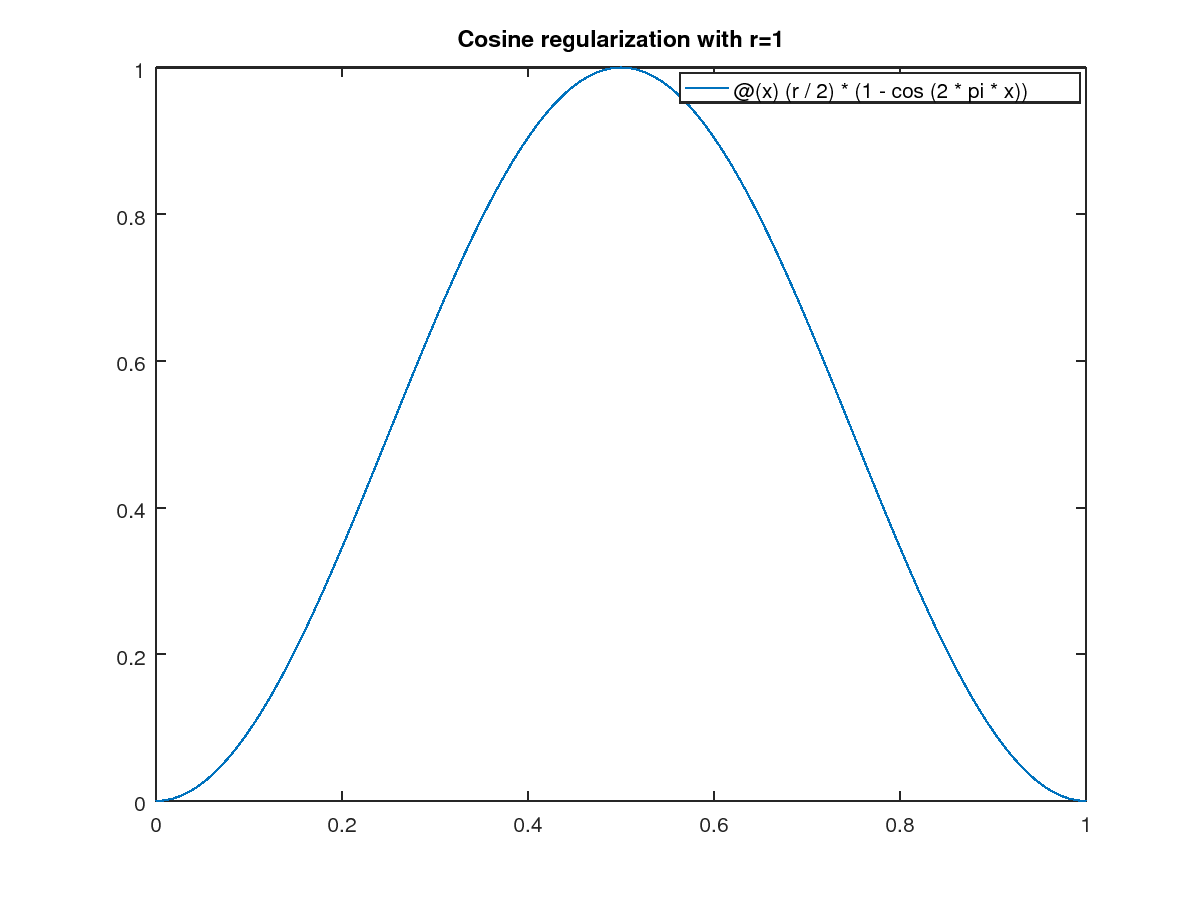
\includegraphics[totalheight=0.45\textheight]{img/cos_regul.png}
	\caption{Cosinus regularization with $r=1$}
	\label{fig:cos_regul}
	
	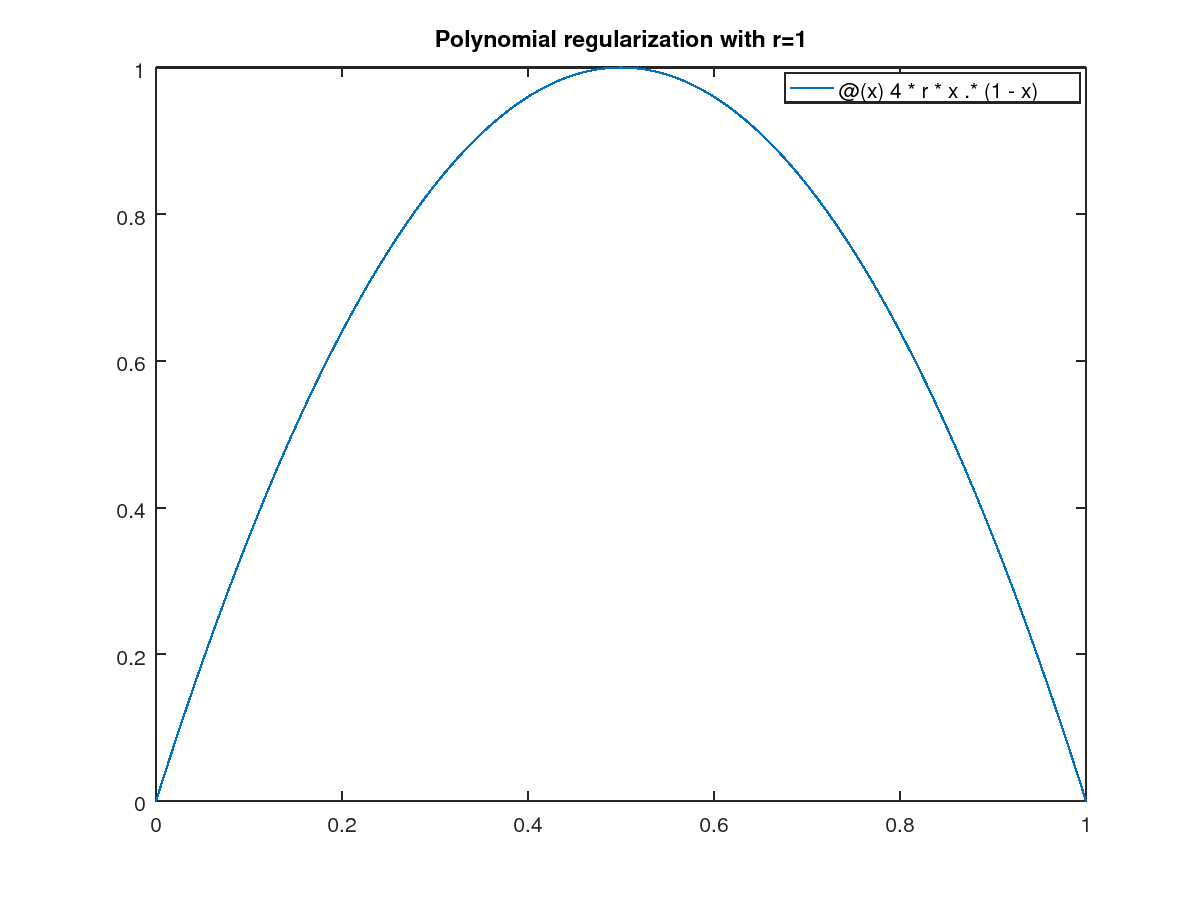
\includegraphics[totalheight=0.45\textheight]{img/poly_regul.png}
	\caption{Polynomial regularization with $r=1$}
	\label{fig:poly_regul}
\end{figure*}

\begin{figure*}
	\centering
	
	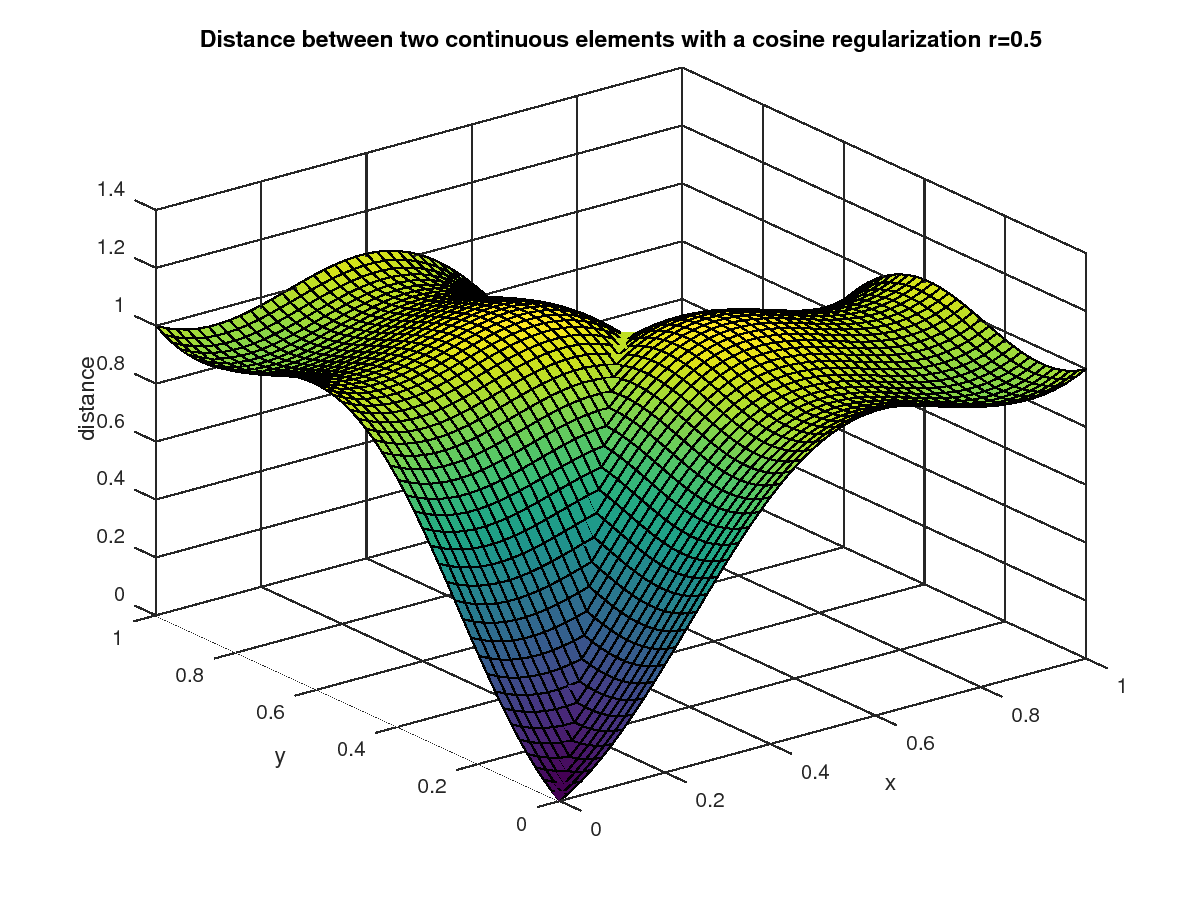
\includegraphics[totalheight=0.4\textheight]{img/distance_regul_cos.png}
	\caption{Distance between two continuous bits with a cosine regularization $r=0.5$}
	\label{fig:distance_regul_cos}
	
	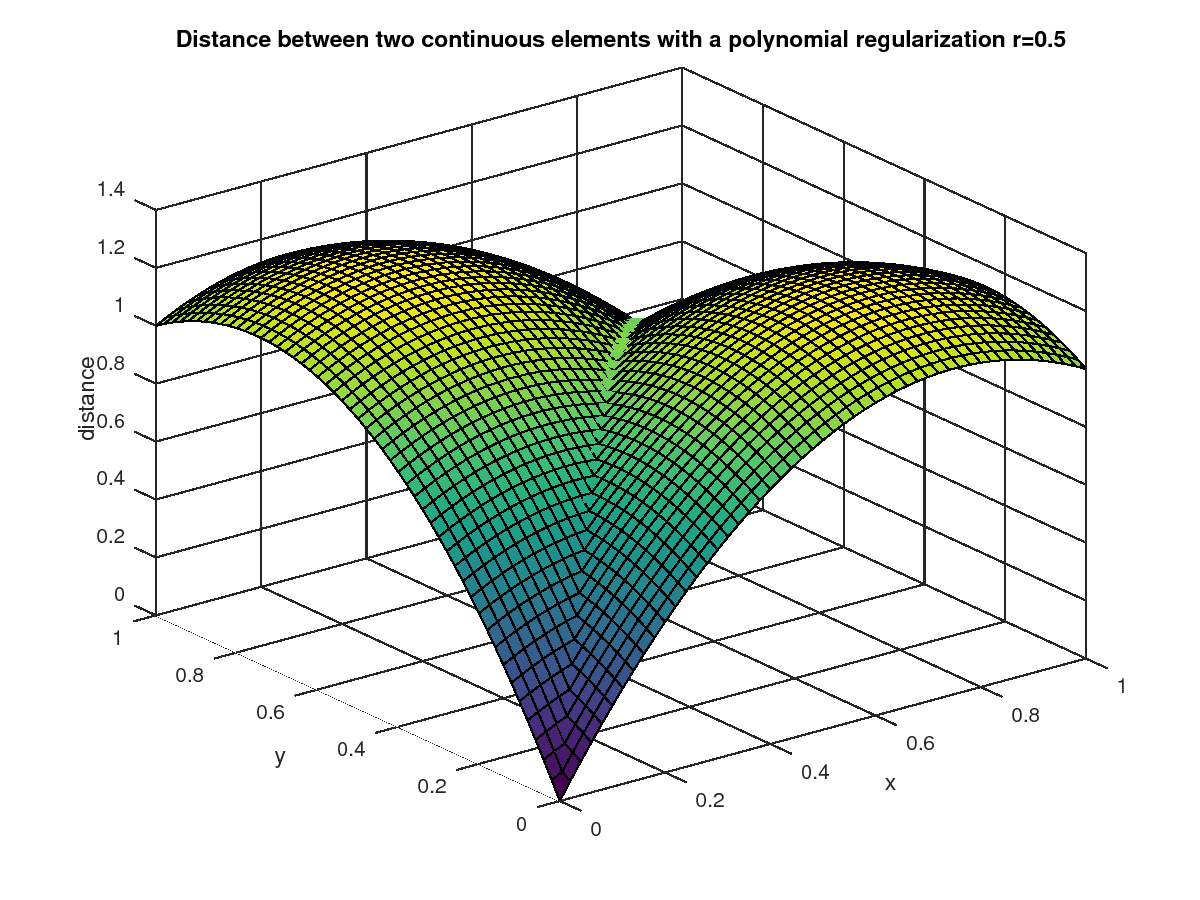
\includegraphics[totalheight=0.4\textheight]{img/distance_regul_poly.png}
	\caption{Distance between two continuous bits with a polynomial regularization $r=0.5$}
	\label{fig:distance_regul_poly}
\end{figure*}

We implemented two types of regularization: cosine (see figure \ref{fig:cos_regul}) and polynomial (see figure \ref{fig:poly_regul}). 

\[R_{cos}(x) = \frac{r}{2}(1-\cos{2\pi x}) \text{ with } r \in \mathbb{R}_{+}\]

\[R_{poly}(x) = 4rx(1-x) \text{ with } r \in \mathbb{R}_{+}\]

Cosine regularization has a null derivative near to 0 and 1 whereas polynomial regularization is steeper in these two regions.

Effect of regularization on the distance function between two continuous bits can be seen in figure \ref{fig:distance_regul_cos} and \ref{fig:distance_regul_poly}. We can see that elements near to 0.5 are penalized, therefore the distance is more than 1. The line between $(0, 0)$ and $(1, 1)$ is distinguishable from the rest of the surface, this originate from the L1 norm in the not regularized distance.

\subsection{Training}
To train the model, we compute the gradient of the cost function and use a gradient descent based method to minimize the cost.

\subsubsection{Gradient of the cost function}
To compute the gradient of the cost function, we first compute the Jacobian of $c_{k;W}(x)$, the sigmoid function.

\[c_{k;W}(x) = sigmoid_k(Wx) = \frac{1}{1 + e^{-kWx}} \text{ with } k \in \mathbb{R}_+\]

As a remainder, the $j$th element of the $i$th input vector is: $c_{k;W}(x_i)_j$. To simplify we note: $c_i = c_{k;W}(x_i)$, $c_{ij} = c_{k;W}(x_i)_j$, $c'_i = c_{k;W}(x'_i)$, $c'_{ij} = c_{k;W}(x'_i)_j$.

\[\frac{\partial c_{k;W}(x)_i}{\partial W_{ij}} = k \times c_{k;W}(x)_i(1 - c_{k;W}(x)_i)x_j\]

We then compute the gradient of the distance with the absolute value function.

\[\norm{c - c'}_{C} = \sum\limits_{i=1}^q \left|c_i-c'_i\right| \text{ with } c, c' \in [0, 1]^{q}\]

\[\frac{\partial \left|c-c'\right|}{\partial W_{ij}} = sgn(c-c')(\frac{\partial c}{\partial W_{ij}} - \frac{\partial c'}{\partial W_{ij}})\]

\[\frac{\partial \norm{c - c'}_{C}}{\partial W_{ij}} = \sum\limits_{i=1}^q sgn(c_i-c'_i)(\frac{\partial c_i}{\partial W_{ij}} - \frac{\partial c'_i}{\partial W_{ij}})\]

We then compute the gradient of the hinge functions.

\[
	\begin{split}
		\frac{\partial max(0, f(W) - \rho)}{\partial W_{ij}} & =
		\begin{cases}
		0                                     & \text{if } f(W) \leq \rho \\
		\frac{\partial f(W)}{\partial W_{ij}} & \text{if } f(W) > \rho
		\end{cases} \\[3ex]
		& = \mathbbm{1}_{f(W) > \rho} \frac{\partial f(W)}{\partial W_{ij}}
	\end{split}
\]

\[
	\begin{split}
		\frac{\partial max(0, \rho - f(W) + 1)}{\partial W_{ij}} & =
		\begin{cases}
		0                                      & \text{if } f(W) \geq \rho + 1 \\
		-\frac{\partial f(W)}{\partial W_{ij}} & \text{if } f(W) < \rho + 1
		\end{cases} \\[3ex]
		& = \mathbbm{1}_{f(W) < \rho + 1} \frac{\partial f(W)}{\partial W_{ij}}
	\end{split}
\]

Finally the gradient of the cost function is:

\[
	L_{continuous}(W) = \sum\limits_{t=1}^N s_t\max(0, \norm{c_t - c'_t}_{C} - \rho) + (1-s_t)\lambda\max(0, \rho - \norm{c_t - c'_t}_{C} + 1)
\]

\[
\begin{split}
	\frac{\partial L_{continuous}(W)}{\partial W_{ij}} = \sum\limits_{t=1}^N & s_t \mathbbm{1}_{\norm{c_t - c'_t}_{C} > \rho} \times sgn(c_{tj} - c'_{tj}) k \left(c_{tj} (1 - c_{tj}) x_{ti} - c'_{tj} (1 - c'_{tj}) x'_{ti} \right) \\
& - (1 - s_t) \lambda \mathbbm{1}_{\norm{c_t - c'_t}_{C} < \rho + 1} \times sgn(c_{tj} - c'_{tj}) k \left(c_{tj} (1 - c_{tj}) x_{ti} - c'_{tj} (1 - c'_{tj}) x'_{ti} \right)
\end{split}
\]

\[
\begin{split}
	\frac{\partial L_{continuous}(W)}{\partial W_{ij}} = \sum\limits_{t=1}^N & \left(s_t \mathbbm{1}_{\norm{c_t - c'_t}_{C} > \rho} - (1 - s_t) \lambda \mathbbm{1}_{\norm{c_t - c'_t}_{C} < \rho + 1}\right) \\
& \times sgn(c_{tj} - c'_{tj}) k \left(c_{tj} (1 - c_{tj}) x_{ti} - c'_{tj} (1 - c'_{tj}) x'_{ti} \right)
\end{split}
\]

The octave code to compute the cost function is in appendix \ref{chapter:OctaveImplementation}. 

\subsubsection{Gradient of the regularization term}
Gradient of the cosine regularization
\[
	R_{cos}(W) = \sum\limits_{i=1}^N \sum\limits_{j=1}^q \frac{r}{2}(1 - \cos(2 \pi c_{ij})) + \frac{r}{2}(1 - \cos(2 \pi c'_{ij}))
\]

\[
\begin{split}
	\frac{\partial R_{cos}(W)}{\partial W_{ij}} = \sum\limits_{t=1}^N &   \pi kr \sin(2 \pi c_{tj}) c_{tj} (1 - c_{tj}) x_{ti} \\
	                                                                  & + \pi kr \sin(2 \pi c'_{tj}) c'_{tj} (1 - c'_{tj}) x'_{ti}
\end{split}
\]

Gradient of the polynomial regularization
\[
	R_{poly}(W) = \sum\limits_{i=1}^N \sum\limits_{j=1}^q 4r c_{ij}(1 - c_{ij}) + 4r c'_{ij}(1 - c'_{ij})
\]

\[
\begin{split}
	\frac{\partial R_{poly}(W)}{\partial W_{ij}} = \sum\limits_{t=1}^N &   4rk (1-2c_{tj}) c_{tj} (1 - c_{tj}) x_{ti}    \\
	                                                                   & + 4rk (1-2c'_{tj}) c'_{tj} (1 - c'_{tj}) x'_{ti}
\end{split}
\]

\subsubsection{Optimization}
The parameters $W$ are initialized using LSH. The elements of $W$ are sampled from a normal density $\mathcal{N}(0, 1)$ and each row is normalized. Our implementation \footnote{https://github.com/mgaillard/PerceptualHashingLearning} use the fminunc function of Octave. It is possible to run the optimization multiple times with different initializations in order to take the best solution. For reproducibility, it is possible to fix the seed before the optimization. Thus, one can run the optimization multiple times with the same initialization.

To monitor the training, the continuous and real costs are displayed before and after gradient descent. If the continuous cost doesn't decrease too much, it is probably because the cost function is too hard to optimize. In this case a decreasing in the value of $k$ could help because it makes the surface of the cost function smoother. After training, a histogram of values of elements in continuous codes is computed. Ideally this histogram would contain an equal amount of values near to 0 or 1. If elements take values between 0 and 1, one could increase the value of $k$ in order to sharpen the sigmoid function, another solution would be to increase the value of $r$ in order to regularize the cost function. However, a too high value for the regularization increases the number of local minima and the cost function becomes harder to minimize. Finally, precision, recall and F-measure are computed on all pairs of images with similarity labels. If the distance between the binary codes of a pair of similar images is less (resp. greater) than $\rho$, it is a true (resp. false) positive. If the distance between the binary codes of a pair of dissimilar images is greater (resp. less) than $\rho$, it is a true (resp. false) negative. There is an example of report generated to monitor the training in appendix \ref{chapter:TrainingReport}.

% ---------------- Section: Experiments ----------------
\section{Experiments}
Experiments are conducted on the Octave implementation.

\subsection{2D points dataset}
As a first experiment, we use a dataset of random 2D points. Indeed, with only 2 dimensions, the points are very easy to visualize. Moreover, in this case hyperplanes are lines parametrized by only two values. It means that if we hash 2D points with only one bit it is possible to plot the surface of the corresponding cost function. This experiment is thus only useful to develop and visually control that our method performs well.

The input dataset is composed of $n$ clouds of $k$ points in 2D. Each cloud of point is centered around a point, whose coordinates are randomly chosen from a uniform distribution between -10 and 10. In other words, clouds are in a square of side 20 centered around the origin. To generate points in clouds, we choose each coordinate from a normal distribution of variance $s$ and whose mean is the center of the cloud. Then we generate an exhaustive list of pairs of points with similarity labels. Similar (resp. dissimilar) points come from the same (resp. different) cloud.

\subsubsection{With two clouds}
The result of our method can be seen in figure \ref{fig:hyper_2d_one_hyperplane_scatter} and the surface of the cost function is in figure \ref{fig:hyper_2d_one_hyperplane_cost}. In this example, we can clearly see that the solution is perfect. No regularization were used, $k=1$ and $\rho=0$, which means that no hyperplane should pass through a cloud.

\begin{figure*}
	\centering
	
	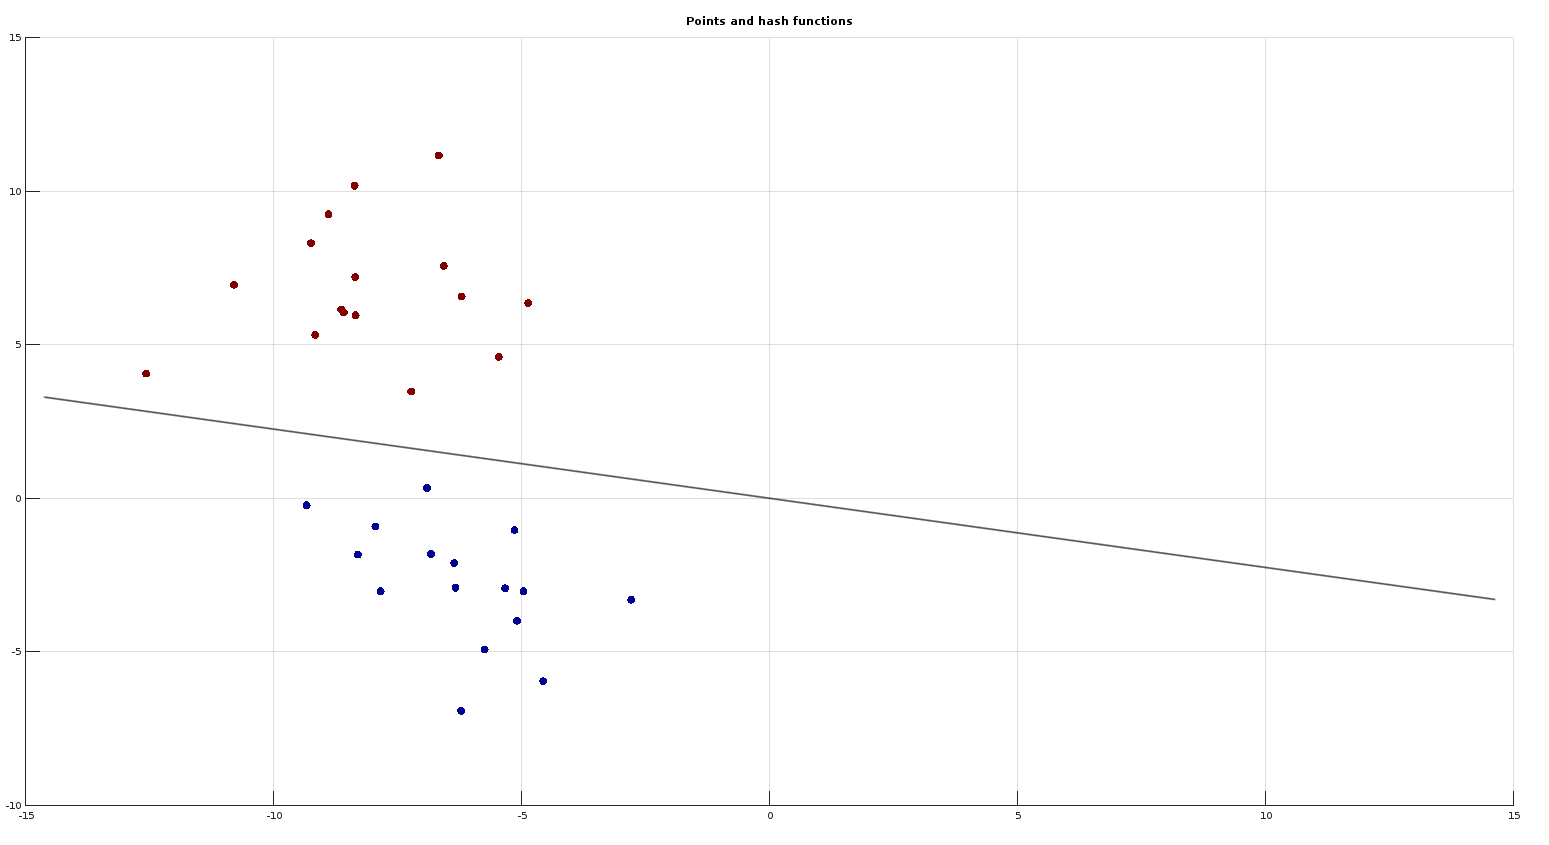
\includegraphics[width=\textwidth]{img/hyper_2d_one_hyperplane_scatter.png}
	\caption{Scatter plot of the dataset with 2 clouds of 16 points. The best hyperplane found is the black line passing through the origin.}
	\label{fig:hyper_2d_one_hyperplane_scatter}
	
	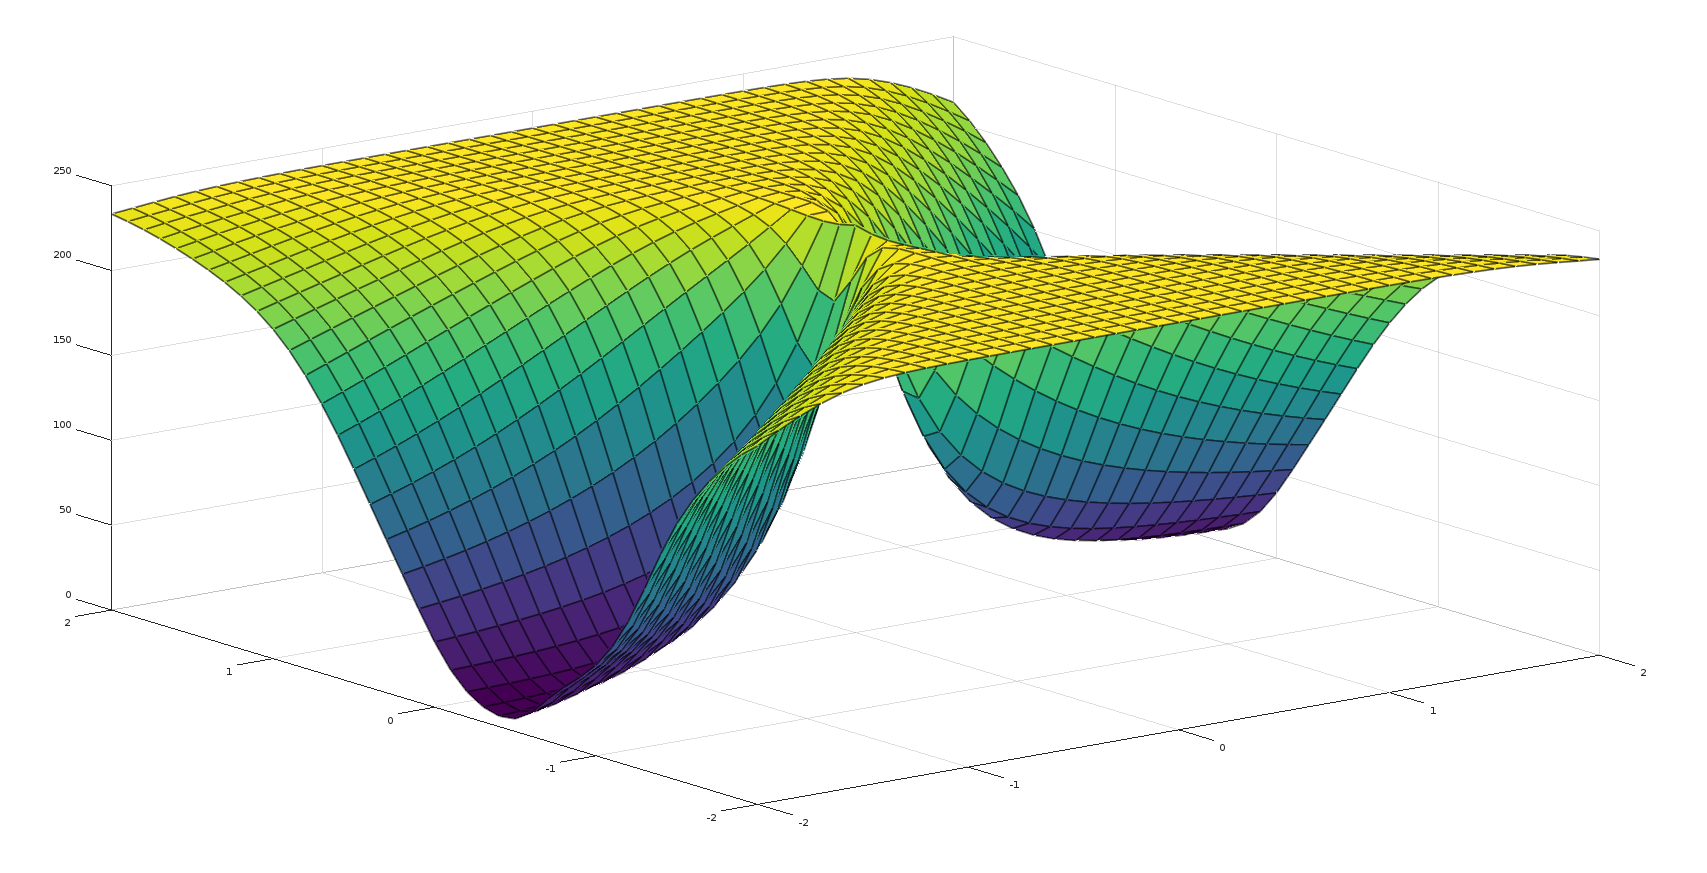
\includegraphics[width=\textwidth]{img/hyper_2d_one_hyperplane_cost.png}
	\caption{Surface of the cost function for one hyperplane in 2 dimensions and a distribution of points shown in figure \ref{fig:hyper_2d_one_hyperplane_scatter}. In this case two regions seem to be optimum.}
	\label{fig:hyper_2d_one_hyperplane_cost}
\end{figure*}

This problem is similar to the linearly separable case of SVM. There is not a maximum margin constraint but the hyperplanes are not too close to the clouds. This is probably due to the fact that the minimization in continuous space has a similar effect. Indeed, the continuous representation is never exactly equal to 0 or 1. Therefore, the optimization will force the continuous representation to take a value nearer to 0 or 1 even if the value is already near to 0 or 1. In other words, the hyperplane will stay away from the points, maximizing the margin between the hyperplane and points.

\subsubsection{With four clouds}
The result of two optimizations on 4 clouds of 16 points can be seen in figures \ref{fig:hyper_2d_three_hyperplane_scatter_easy} and \ref{fig:hyper_2d_three_hyperplane_scatter_hard}. No regularization were used, $k=1$ and $\rho=0$. The first figure \ref{fig:hyper_2d_three_hyperplane_scatter_easy} shows a case where the solution is perfect. In this particular case, only two hyperplanes would have been enough. The second figure \ref{fig:hyper_2d_three_hyperplane_scatter_hard} shows a case where a local optimum is found. One hyperplane passes through the yellow cloud. This is possible because, from the point of view of the cost function, a value of 0.5 for two similar points is considered as satisfying because no regularization is applied. 

\begin{figure*}
	\centering
	
	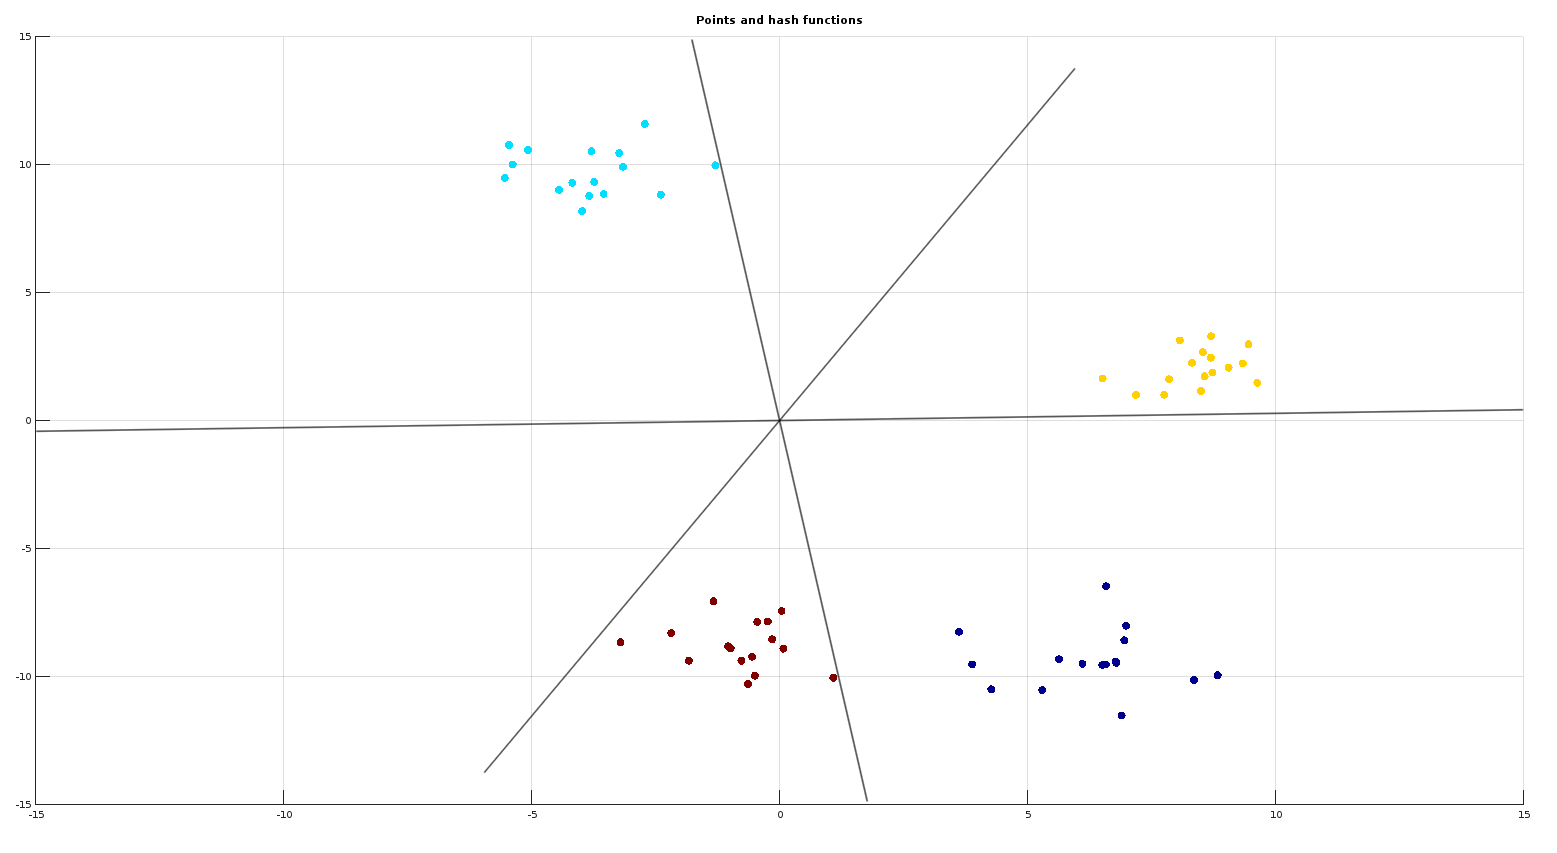
\includegraphics[width=\textwidth]{img/hyper_2d_three_hyperplane_scatter_easy.png}
	\caption{Scatter plot of the dataset with 4 clouds of 16 points. The best hyperplanes found are the black lines passing through the origin.}
	\label{fig:hyper_2d_three_hyperplane_scatter_easy}
	
	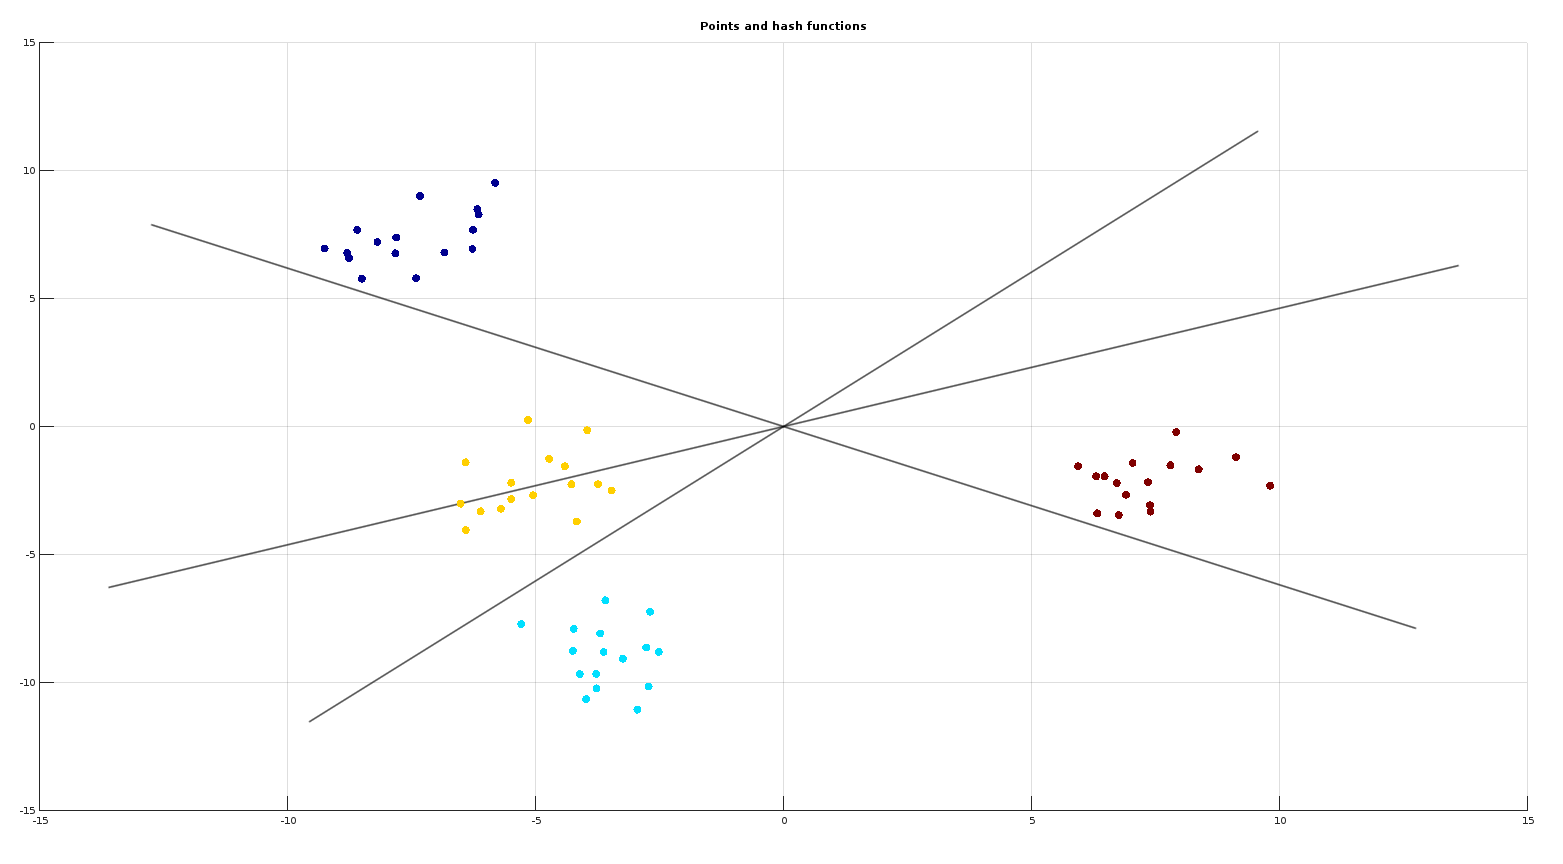
\includegraphics[width=\textwidth]{img/hyper_2d_three_hyperplane_scatter_hard.png}
	\caption{Scatter plot of the dataset with 4 clouds of 16 points. The best hyperplanes found are the black lines passing through the origin. Here one hyperplane passes through a cloud.}
	\label{fig:hyper_2d_three_hyperplane_scatter_hard}
\end{figure*}

\subsection{CNN Features dataset}
We extract features with \textit{VGG16\_block5\_pool\_max} because it has at the same time good retrieval performances and a low number of dimensions. It is desirable because the computation of the cost function is easier when features have less dimensions. 

To evaluate the quality of the hashing, we use an adaptation of our benchmark, in chapter \ref{chapter:Benchmarking}. We use the $n$ first images of MIRFLICKR \footnote{http://press.liacs.nl/mirflickr/} and their $K=6$ modified versions according to the modifications listed in section \ref{chapter:Benchmarking:section:Protocol}: blur, grayscale, resize, JPEG compression, rotation and cropping. So we have $N=(K+1)n$ images in total. The input dataset is composed of all $N(N-1)/2$ pairs of images along with their similarity labels. A pair of images that both come from the same base image is considered as similar. In the same way, a pair of images that don't come from the same base image is considered as dissimilar. So there are $n*(K+1)K/2$ similar pairs and $N(N-k-1)/2$ dissimilar pairs. Because there is too many dissimilar pairs in comparison to similar pairs, we adapt lambda so that $\lambda=K/(N-K-1)$. CNN Features are mean-centered (all at the same time) and then normalized to unit length in L2. Once training is finished, we predict the binary codes of all $N$ images and run the benchmark on the codes. It is important to note that there is no validation and test set. We learn our hash function from the actual data, thus overfitting is not a problem. Finally, we compare the precision, recall and F-measure of generated binary codes in Hamming distance to raw features with cosine distance.

Ideally, binary codes would have the same retrieval performance as raw features. It is even possible that binary codes perform better than raw features. Indeed, similarity labels stem from classes of images and not from the cosine distance between their representations. Therefore, even if angular distance is not perfect to compare image representations, it is possible to find a partitioning of the space that leads to perfect binary codes. In this particular case, the hash function learns to correct the mistakes of the image representations. This approach would be also applicable to learn the semantic similarity in a classification task. In this case, a nearest neighbor classifier would be used on the learnt binary codes.

\subsubsection{Comparison with LSH}
In this section, we compare the performances of our method to random projection. In theory, our method should perform at least as well as LSH with random projection because it is initialized exactly like LSH. We take the best model over 20 iterations for our method, and the best model over 1000 iterations for LSH. In both cases the seed is initialized with the same value. We hash the $n=50$ first images of MIRFLICKR and their modified versions (so $N=350$) on 16-bits binary codes with $\rho=3$, $k=1$ and no regularization. We plot the histogram of real cost for both methods.

\begin{table}
	\centering
	\caption{Comparison of retrieval performances of our method against LSH with random projection}
	\label{table:lsh_vs_hyper}
	\begin{tabular}{|lrrrrr|}
	\hline
	Method     & Real cost & Radius & Precision & Recall & Fmeasure \\
	\hline                          
	LSH        &       797 &  0,18 &      0,75 &   0,51 &     0,56 \\
	Our method &      21.7 &  0,18 &      0,99 &   0,92 &     0,95 \\
	\hline
	\end{tabular}
\end{table}

\begin{figure}
	\centering
	
	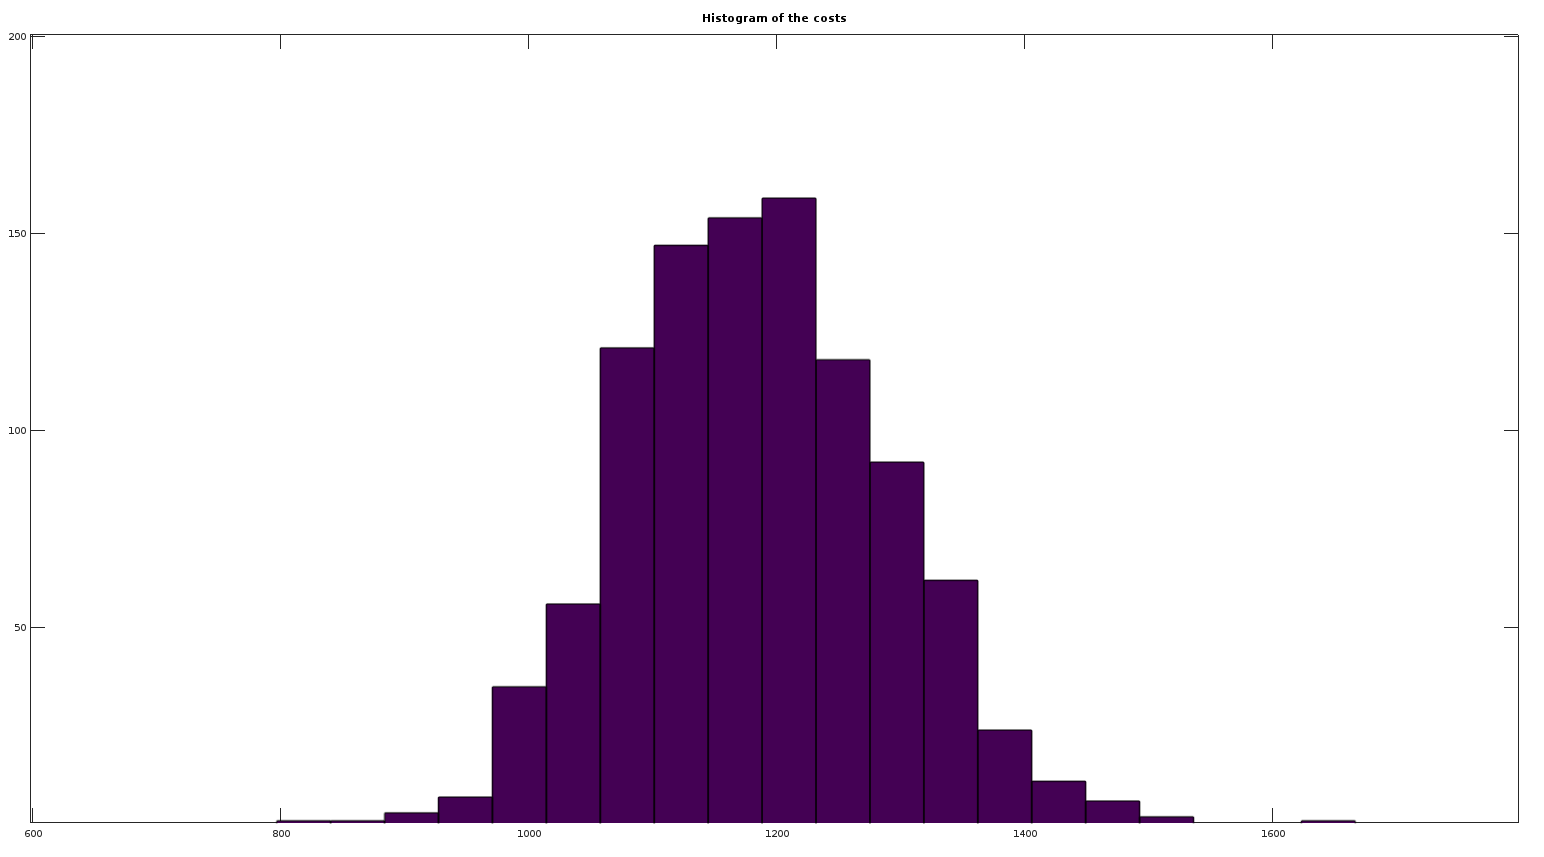
\includegraphics[width=\textwidth]{img/lsh_best_of_1000.png}
	\caption{Histogram of real cost for 1000 iterations of LSH.}
	\label{fig:lsh_vs_hyper_best_of_1000}
\end{figure}

Results are in table \ref{table:lsh_vs_hyper}. The histogram of cost function for LSH is shown in figure \ref{fig:lsh_vs_hyper_best_of_1000}, the mean cost is 1184 and the standard deviation is 106. With 1000 iterations, we can say that LSH is not likely to produce solutions that are really better than the one that we found with the minimal cost of 797. So the F-measure of 0,56 obtained with LSH is a upper bound of the performance of LSH. Our method achieves every time a better solution than LSH with a maximum real cost of 81. The mean real cost is 37.8, the standard deviation is 14.8 and the minimum real cost is 21.7. We can see that our method achieves every time a higher F-measure than LSH with random projection. By the way, it is interesting to note that the best F-measure is reached with a radius of 0.18, which is approximately equal to $\rho / 16$.

% ---------------- Section: Conclusion ----------------
\section{Conclusion}
In this chapter, we present a new approach to learn a hash function for CNN Features. Although our experiments are superficial and can't prove that our method yields state of the art performances, we have very promising results. With more time, we could have conducted more experiments. Some questions are still open: what is the influence of the regularization? How well our method performs when the number of bits increases, when the number of images increases?

The effect of regularization on the distance between two continuous elements could be better. Cosine regularization seems to introduce local minima in the cost function, thus the solutions are often worse with regularization. We didn't extensively test the polynomial regularization, but this one seems to introduce less local minima than cosine regularization. For the moment by choosing the right value for $k$, the regularization is not necessary, but this is a complicated process.

The $k$ parameter is redundant because rows of $W$ are unconstrained, they can take a big value, which is equivalent to a big $k$. We need to evaluate the effect of $k$ and whether it is really required. There seems to be two options, either we keep $k$ and we normalize the rows of $W$, or we remove $k$ and we don't normalize $W$. 

Because our implementation uses the fminunc function of Octave, we can't have an effect on the minimization of the cost function. What we could do is to plot the real cost along with the continuous cost during learning, in order to monitor the optimization. We could also change the pairs of images in the dataset during the training to select at each step only the pairs that bring the more information.

During the training, we select the best model over multiple iterations by choosing the one with the minimum real cost. However, it is not proven that selecting the lowest real cost is equivalent to selecting the highest F-measure. 

The optimization is not easy, the algorithm often falls into a local optimum and to find a satisfying optimum we need to rerun several times the gradient descent with various random inputs. Is it possible to use another optimization method that is less prone to falling in local minima? If we add hidden layers before the hashing layer, shall it be easier to optimize? In facts, the hidden layers can change the input space to ease the training of the last layer. At the end, the objective would be to program a loss layer with a neural network framework. This would allow us to use it on top of a neural network and learn non-linear projections. Moreover, we could use the GPU implementation of the framework to fasten the computation of the cost function.

Scalability is not perfect because the number of pairs of images grows quadratically. For this reason, the number of images is deliberately low because the cost function is hard to compute with a big dataset. For example, with a total of 1400 images, there is about 1 million pairs of images, which is huge. With a GPU implementation, we could go further but definitively not up to a big number of images. Another solution that we explored is to select only the pairs of images that bring the more information, because dissimilar triplets are mostly redundant. Unfortunately, we didn't have the time to evaluate extensively this option. Currently the way to apply this method to large scale reverse image search is to train the model on a small number of images with a validation set and hope that it will generalize on more images.

%  Conclusions (Zusammenfassung):
\chapter{Conclusion}

\label{chapter:Conclusion}

% ----------------

In this thesis, we present our study on Convolutional Neural Networks Features and Perceptual Hashing for Large Scale Reverse Image Search. A potential application is to find near-duplicate in large collections of images.

To implement an actual reverse image search system with the content of this thesis, one can make use of the CNN Features described in chapter \ref{chapter:CNNFeaturesRobustness} to represent images, followed by the use of the method developed in chapter \ref{chapter:CNNFeaturesHashing} to learn a hash function that maps CNN Features into short binary codes, finally techniques described in chapter \ref{chapter:SearchHammingSpace} can be used to perform efficient nearest neighbor searches on binary codes.

In the review part, we describe what is reverse image search and common methods to tackle this problem. We also advocate the use of convolutional neural networks to represent images, and hashing into binary codes to facilitate nearest neighbor search.

The potential of CNN Features for reverse image search, even with slight modifications, is proven. Image representations extracted with convolutional neural networks on unrelated classification tasks are considerably robust against modifications. We didn't expressly compared CNN Features against other state of the art descriptors, but our experiments, along with the content of other publications presented in chapter \ref{chapter:ConvolutionalNeuralNetworks}, tend to prove that CNN Features are state of the art descriptors for reverse image search and more generally for image retrieval.

We propose a method to learn a hash function that maps features into short binary codes while preserving similarity. This method is inspired from Minimal Loss Hashing, described in chapter \ref{chapter:HashingDimensionalityReduction}, but uses a new approach to optimize the cost function. We keep the codes continuous during learning, this allows us to compute the gradient of the cost function it minimize it. Although our experiments are superficial and can't prove that our method yields state of the art performances, we have very promising results. With more time, we could improve our method and evaluate its performances in comparison with state of the art techniques. Interesting directions are exhibited in the conclusion of chapter \ref{chapter:CNNFeaturesHashing}.

We foresee the implementation of our method as a loss layer in a neural network framework to promise excellent results. Firstly, this would allow us to benefit from the computational power of GPU, secondly, we would be able to add hidden layers to learn non-linear projections, and finally, the joint learning of the image representation and the hash function would yield even better results.

% Appendix (Anh�nge), could have multiple chaper-files:
\appendix
\chapter{Implementation of DCT-based perceptual hash}

\label{chapter:ImplementationDCTPerceptualHash}

% ----------------

During our project, we implemented a version of the DCT based perceptual hash function with OpenCV. This one has the same retrieval performance than the original one in \cite{zauner2010implementation} and is faster.

\lstset{
	language=C++,
	breaklines=true,
  postbreak=\mbox{\textcolor{red}{$\hookrightarrow$}\space}
}
\begin{lstlisting}
#include <opencv2/core/core.hpp>
#include <opencv2/highgui/highgui.hpp>
#include <opencv2/imgproc/imgproc.hpp>
#include <string>
#include <cstdint>

uint64_t DctPerceptualHash(const std::string& file_path)
{
    uint64_t hash = 0;
    cv::Mat input;
    cv::Mat grayImg;
    cv::Mat bluredImg;
    cv::Mat resizeImg;
    cv::Mat resizeFImg;
    cv::Mat dctImg;

    input = cv::imread(file_path);

    if (input.data == NULL || (input.type() != CV_8UC3 && input.type() != CV_8U)) {
        // If there is a reading error, return a null hash.
        cerr << "Error reading image" << endl;
        return 0;
    }

    // Convert the image to grayscale using its luminance
    if(input.type() == CV_8UC3) {
        cv::cvtColor(input, grayImg, CV_BGR2GRAY);
    } else {
        grayImg = input;
    }

    // Mean filter with kernel 7x7.
    cv::blur(grayImg, bluredImg, cv::Size(7, 7));

    // Resize the image to 32x32 pixels.
    cv::resize(bluredImg, resizeImg, cv::Size(32,32));

    resizeImg.convertTo(resizeFImg, CV_32F);
    cv::dct(resizeFImg, dctImg);

    std::vector<float> topLeftCoeffs;
    // Take only the coeffs in rectangle (1, 1) ; (9, 9)
    topLeftCoeffs.reserve(64);
    for (int i = 1; i <= 8; i++) {
        for (int j = 1; j <= 8; j++) {
            topLeftCoeffs.push_back(dctImg.at<float>(i, j));
        }
    }

    // Compute the median
    std::vector<float> coeffs(topLeftCoeffs);

    // The median of a 64 elements array is the mean between the 31th and the 32th element.
    float median = 0;
    std::nth_element(coeffs.begin(), coeffs.begin() + coeffs.size()/2, coeffs.end());
    median += coeffs[coeffs.size()/2];
    std::nth_element(coeffs.begin(), coeffs.begin() + coeffs.size()/2 - 1, coeffs.end());
    median += coeffs[coeffs.size()/2 - 1];
    median /= 2;

    // Transform into a 64 bits integer.
    for (int i = 0; i < topLeftCoeffs.size(); i++) {
        hash <<= 1;
        if (topLeftCoeffs[i] >= median) {
            hash |= 1;
        }
    }

    return hash;
}
\end{lstlisting}
\chapter{Detailed results of VGG16\_block5\_pool\_max with Cosine distance}

\label{chapter:ResultsVGG16Block5PoolMax}

% ----------------

In this appendix, we present the detailed results of the benchmark for \textit{VGG16\_block5\_pool\_max} with Cosine distance.

\begin{figure*}
	\centering
	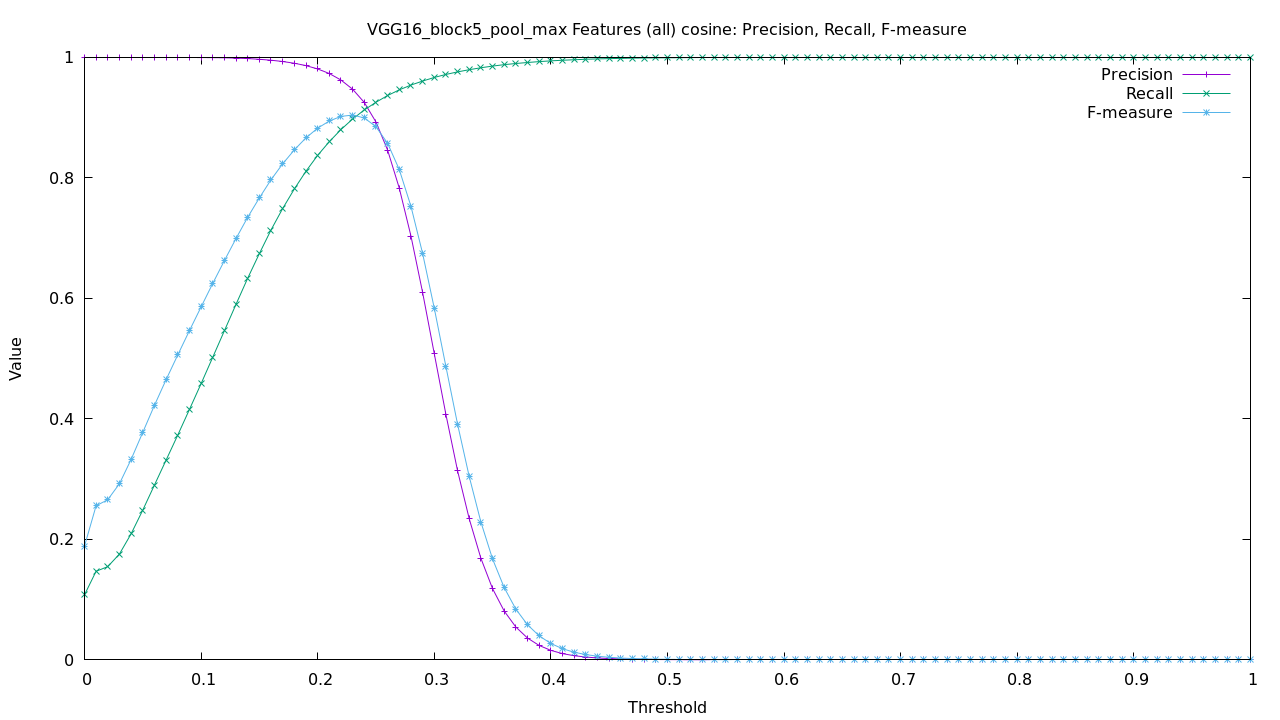
\includegraphics[width=\textwidth]{img/benchmark_VGG16_block5_pool_max_cosine_all.png}
	\caption{Precision, recall, Fmeasure, curves of \textit{VGG16\_block5\_pool\_max} search results with all modifications according to different radius (threshold).}
	\label{fig:benchmark_VGG16_block5_pool_max_cosine_all}
\end{figure*}

\begin{figure*}
	\centering
	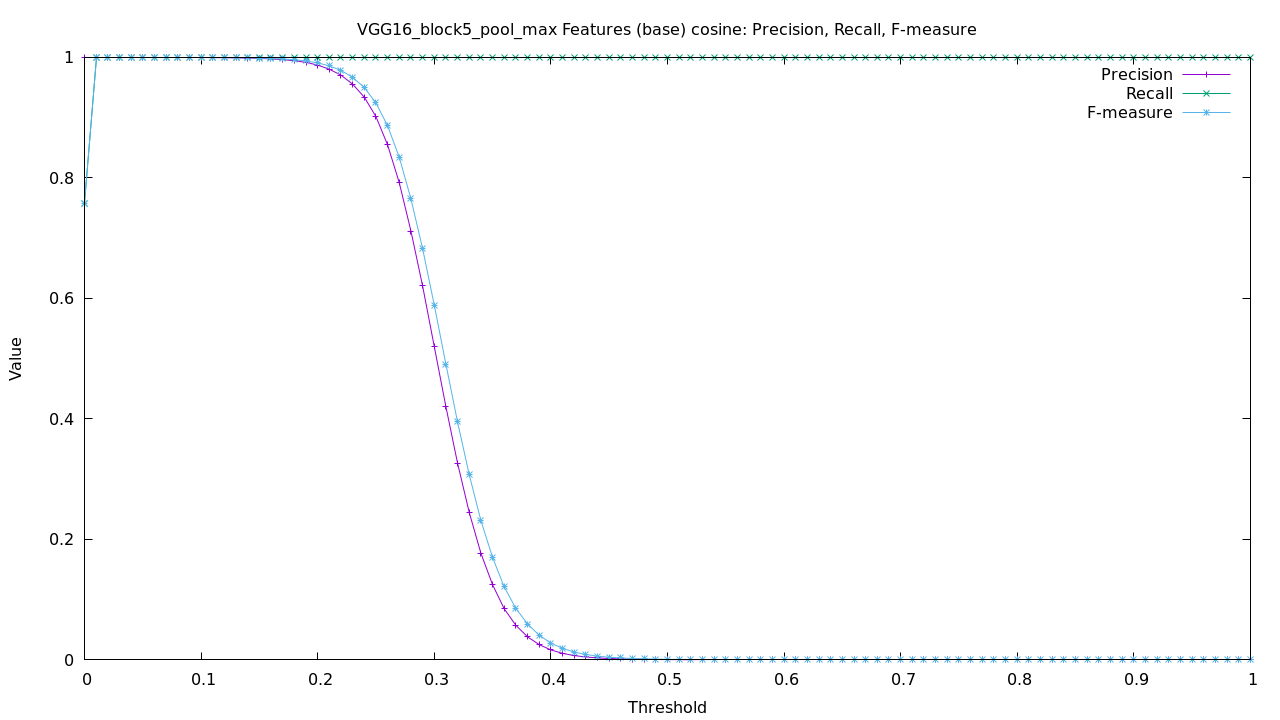
\includegraphics[width=\textwidth]{img/benchmark_VGG16_block5_pool_max_cosine_base.png}
	\caption{Precision, recall, Fmeasure, curves of \textit{VGG16\_block5\_pool\_max} search results with no modification according to different radius (threshold).}
	\label{fig:benchmark_VGG16_block5_pool_max_cosine_base}
\end{figure*}

\begin{figure*}
	\centering
	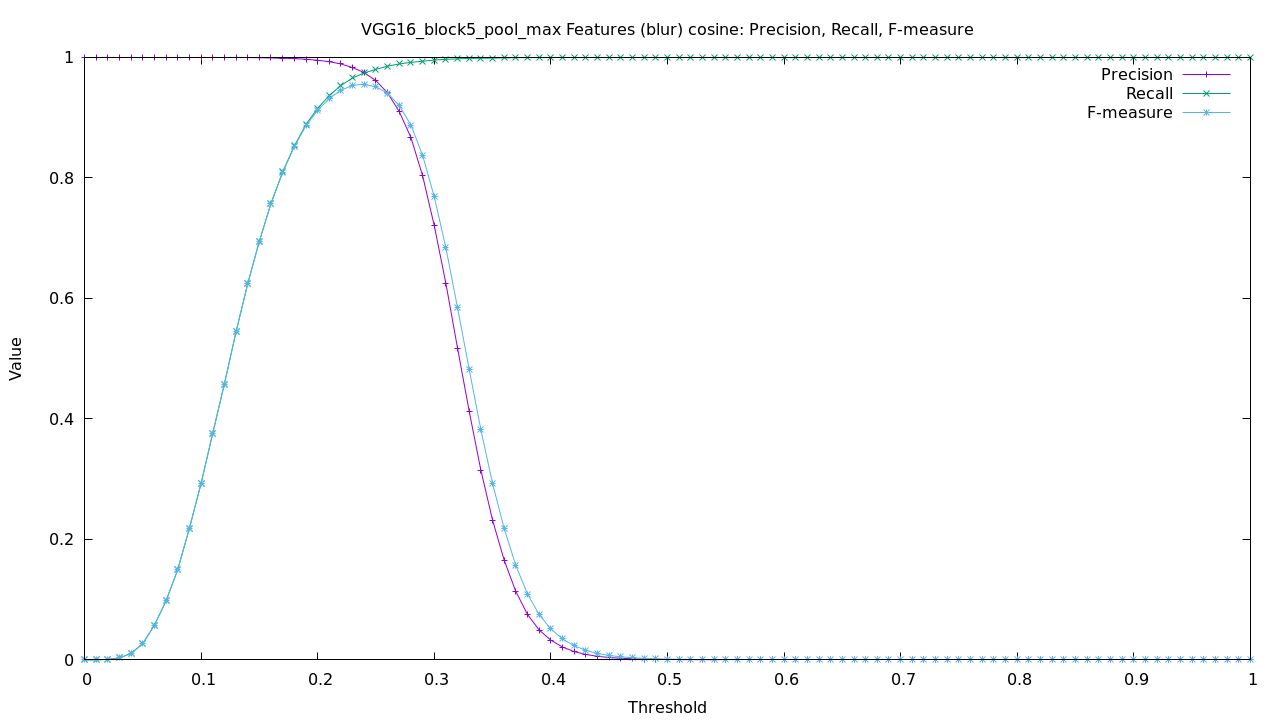
\includegraphics[width=\textwidth]{img/benchmark_VGG16_block5_pool_max_cosine_blur.png}
	\caption{Precision, recall, Fmeasure, curves of \textit{VGG16\_block5\_pool\_max} search results only with Gaussian blur ($r=4$, $\Sigma=2$) according to different radius (threshold).}
	\label{fig:benchmark_VGG16_block5_pool_max_cosine_blur}
\end{figure*}

\begin{figure*}
	\centering
	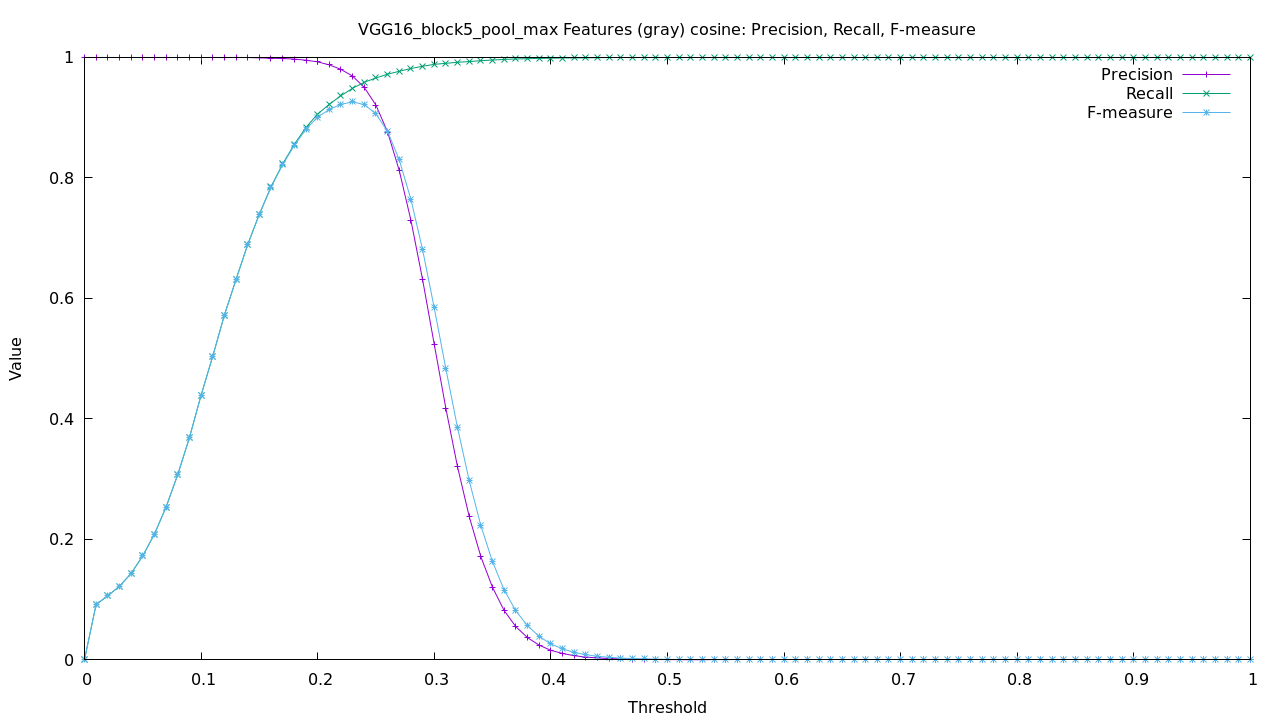
\includegraphics[width=\textwidth]{img/benchmark_VGG16_block5_pool_max_cosine_gray.png}
	\caption{Precision, recall, Fmeasure, curves of \textit{VGG16\_block5\_pool\_max} search results only with grayscale filter according to different radius (threshold).}
	\label{fig:benchmark_VGG16_block5_pool_max_cosine_gray}
\end{figure*}

\begin{figure*}
	\centering
	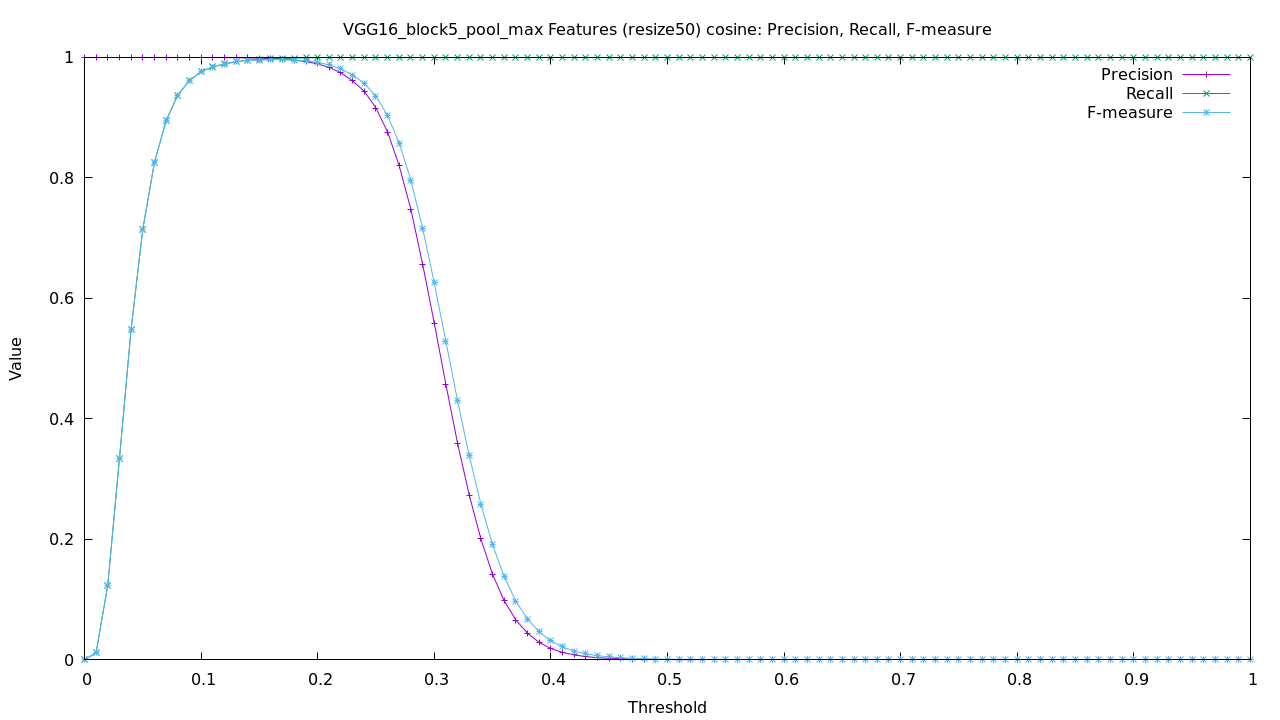
\includegraphics[width=\textwidth]{img/benchmark_VGG16_block5_pool_max_cosine_resize50.png}
	\caption{Precision, recall, Fmeasure, curves of \textit{VGG16\_block5\_pool\_max} search results only with resize to half size according to different radius (threshold).}
	\label{fig:benchmark_VGG16_block5_pool_max_cosine_resize50}
\end{figure*}

\begin{figure*}
	\centering
	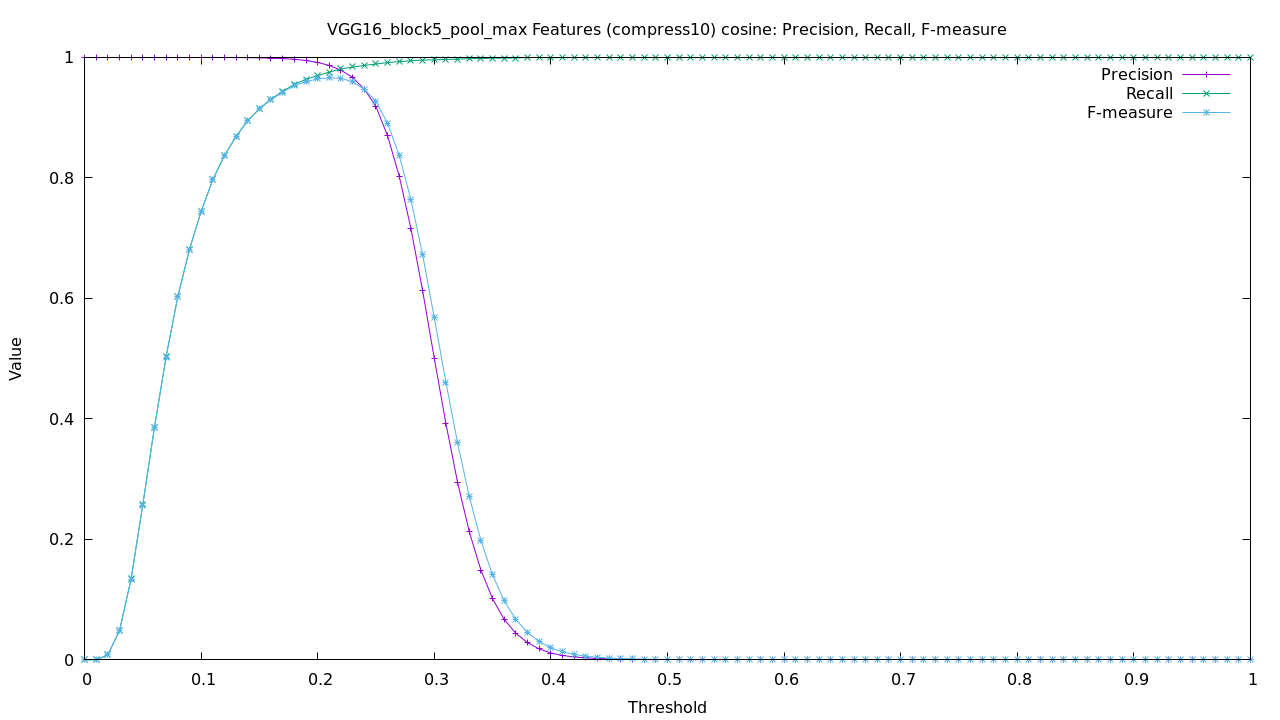
\includegraphics[width=\textwidth]{img/benchmark_VGG16_block5_pool_max_cosine_compress10.png}
	\caption{Precision, recall, Fmeasure, curves of \textit{VGG16\_block5\_pool\_max} search results only with JPEG compression (quality 10\%) according to different radius (threshold).}
	\label{fig:benchmark_VGG16_block5_pool_max_cosine_compress10}
\end{figure*}

\begin{figure*}
	\centering
	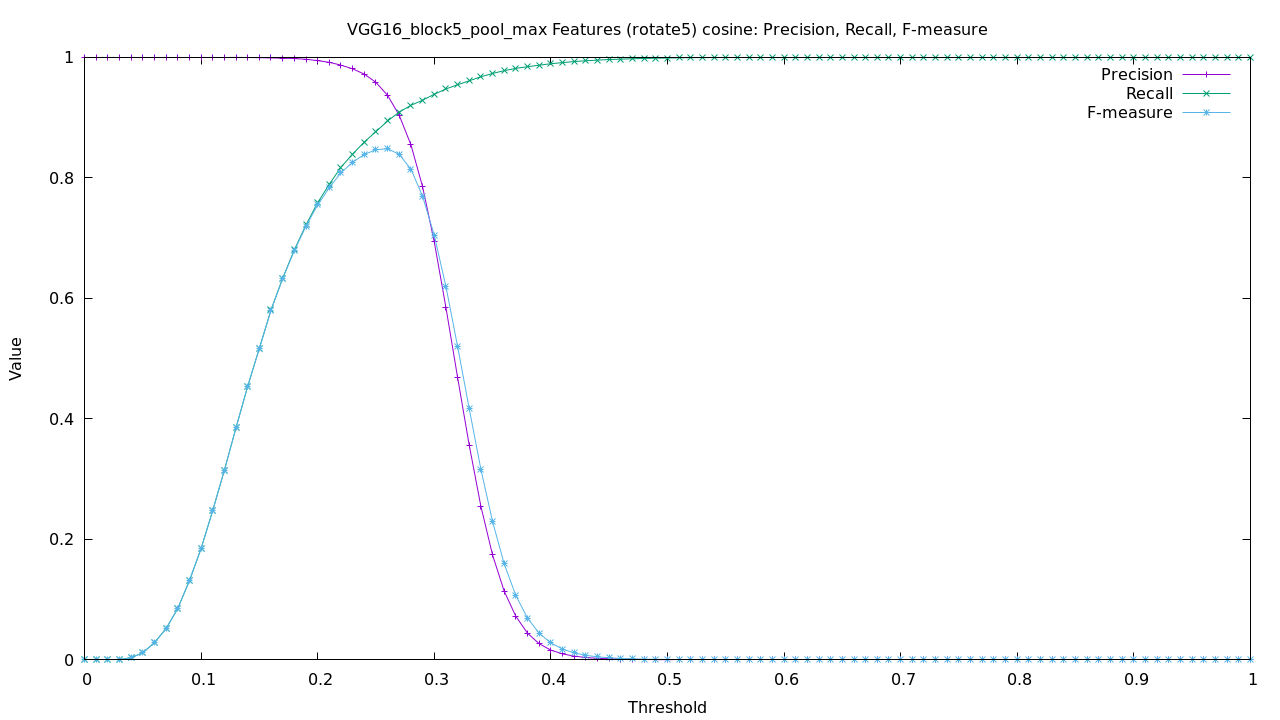
\includegraphics[width=\textwidth]{img/benchmark_VGG16_block5_pool_max_cosine_rotate5.png}
	\caption{Precision, recall, Fmeasure, curves of \textit{VGG16\_block5\_pool\_max} search results only with clockwise rotation by 5 degrees according to different radius (threshold).}
	\label{fig:benchmark_VGG16_block5_pool_max_cosine_rotate5}
\end{figure*}

\begin{figure*}
	\centering
	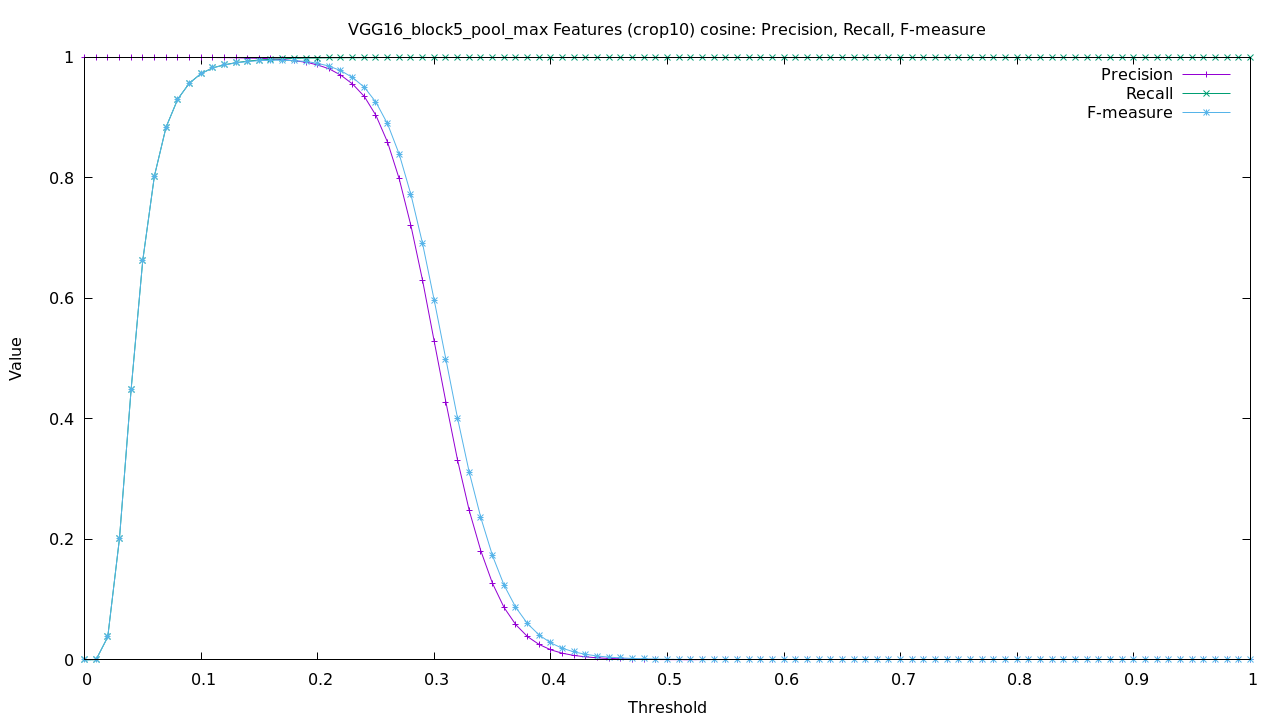
\includegraphics[width=\textwidth]{img/benchmark_VGG16_block5_pool_max_cosine_crop10.png}
	\caption{Precision, recall, Fmeasure, curves of \textit{VGG16\_block5\_pool\_max} search results only with cropping by 10\% at the right side of the image according to different radius (threshold).}
	\label{fig:benchmark_VGG16_block5_pool_max_cosine_crop10}
\end{figure*}
\chapter{Octave Implementation}

\label{chapter:OctaveImplementation}

% ----------------

\lstset{
	language=Octave,
	breaklines=true,
  postbreak=\mbox{\textcolor{red}{$\hookrightarrow$}\space}
}
\begin{lstlisting}
% Compute the cost and the gradient of a set of parameters W
% X1, X2 are input vectors and S is a similarity vector
% S(i) == 1 means that X1(i) and X2(i) are similar
% k, rho, lambda, regularization are hyper parameters of the cost function
function [cost grad] = HyperModel_ContinuousCostFunction(X1, X2, W, S, k, rho, lambda, regularization)
% Binary codes of the samples
a1 = 1.0 ./ (1.0 + exp(-k*X1*W));
a2 = 1.0 ./ (1.0 + exp(-k*X2*W));

% Hamming distance between the two binary codes.
Diff = a1 - a2;
HammingDist = sum(abs(Diff), 2);

% ---------- Cost ----------

cost = sum(S.*max(0, HammingDist - rho) + (1-S).*lambda.*max(0, (rho+1) - HammingDist));

% Regularization of activations
if (regularization > 0)
	% Cosine regularization
	% cost += sum(sum((regularization/2)*(1 - cos(2*pi*a1))));
	% cost += sum(sum((regularization/2)*(1 - cos(2*pi*a2))));
	
	% Polynomial regularization
	cost += sum(sum(4*regularization*a1.*(1 - a1)));
	cost += sum(sum(4*regularization*a2.*(1 - a2)));
endif

% ---------- Gradient ----------

DiffSign = sign(Diff);
HingeSimilar = [HammingDist > rho];
HingeDissimilar = [HammingDist < (rho+1)];

grad = X1'*(S .* HingeSimilar .* DiffSign .* k .* a1 .* (1 - a1)) ...
		 - X2'*(S .* HingeSimilar .* DiffSign .* k .* a2 .* (1 - a2)) ...
		 - X1'*((1-S) .* lambda .* HingeDissimilar .* DiffSign .* k .* a1 .* (1 - a1)) ...
		 + X2'*((1-S) .* lambda .* HingeDissimilar .* DiffSign .* k .* a2 .* (1 - a2));
		 
% Gradient of the regularization term
if (regularization > 0)
	% Cosine regularization
	% grad += X1'*(regularization*pi*sin(2*pi*a1) .* k .* a1 .* (1 - a1)) ...
	%       + X2'*(regularization*pi*sin(2*pi*a2) .* k .* a2 .* (1 - a2));
	
	% Polynomial regularization
	grad += X1'*(4*regularization*(1 - 2*a1) .* k .* a1 .* (1 - a1)) ...
				+ X2'*(4*regularization*(1 - 2*a2) .* k .* a2 .* (1 - a2));
endif
end
\end{lstlisting}
\chapter{Training Report}

\label{chapter:TrainingReport}

% ----------------

\begin{figure*}
	\centering
	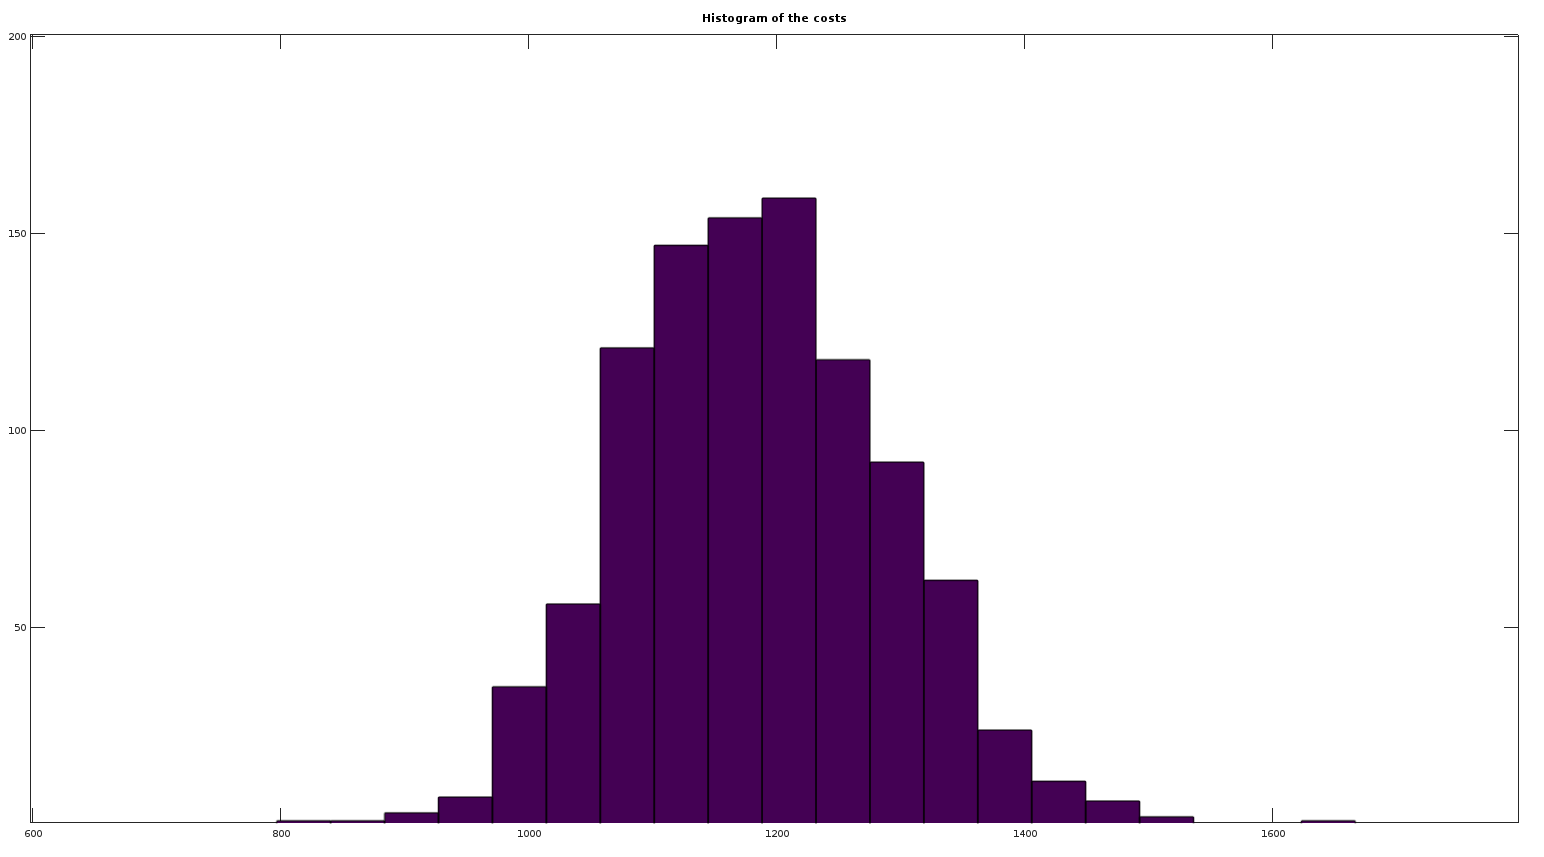
\includegraphics[width=\textwidth]{img/lsh_best_of_1000.png}
	\caption{Histogram of the real cost of 1000 iterations of LSH}
	\label{fig:lsh_best_of_1000}
\end{figure*}

\lstset{
	language={},
	breaklines=true,
  postbreak=\mbox{\textcolor{red}{$\hookrightarrow$}\space}
}
\begin{lstlisting}
initial_cont_cost =  3000.3
initial_real_cost =  1006.0
optimal_real_cost =  27.985
optimal_cont_cost =  0.020816

------ Real cost statistics: ------
Min: 27.9854
Max: 64.9679
Median: 55.3994
Mean: 49.4509
Standard deviation: 19.1954

------ Analysis ------
Middle activation: 1721
Number of training samples: 61075
Number of similar triplets: 1050
Number of dissimilar triplets: 60025
Ratio of similar triplets: 0.017192
Number of true positives: 1031
Number of false positives: 278
Number of false negatives: 19
Number of false negatives: 59747
Ratio of preserved similar triplets: 0.981905
Ratio of preserved dissimilar triplets: 0.995369
Precision: 0.787624
Recall: 0.981905
F1-measure: 0.874099
\end{lstlisting}

% List of figures (Abbildungsverzeichnis):
\listoffigures
% List of tables (Tabellenverzeichnis):
\listoftables
% Glossary (Glossar):
%\include{Glossary}
% List of formulae (Liste der Formelzeichen):
%\include{Formulae}
% Abbreviations (Abk�rzungsverzeichnis):
%\include{Abbreviations}

% References (Literaturverzeichnis):
% a) Style (with numbers: use unsrt):
\bibliographystyle{alpha}
% b) The File:
\bibliography{Bibliography}


%%%%%%%%%%%%%%%%%%%%%%%%%%%%%%%%%%%%%%%%%%%%%%%%%%%%%%%%%%%%


%%%%%%%%%%%%%%%%%%%%%%%%%%%%%%%%%%%%%%%%%%%%%%%%%%%%%%%%%%%%


%%%%%%%%%%%%%%%%%%%%%%%%%%%%%%%%%%%%%%%%%%%%%%%%%%%%%%%%%%%%
\end{document}
